\vspace{-2cm} % Push content upward
\chapter{Iterations}
\label{chap:Iterations}
\vspace{-1cm} % Push content upward

This chapter presents the constructive phase of the research, organized into four development iterations under the Design Science Research (DSR) methodology. The purpose of these iterations is to gradually design and refine a benchmarking pipeline for evaluating the emotion recognition capabilities of large language models across multiple levels of label granularity. Each cycle builds on the previous one, moving from data preparation to context optimization, retrieval-guided prompting, and finally to a unified hybrid system. The progression ensures that every design choice is empirically validated before being integrated into the final artifact.
\begin{figure}[htbp]
    \centering
    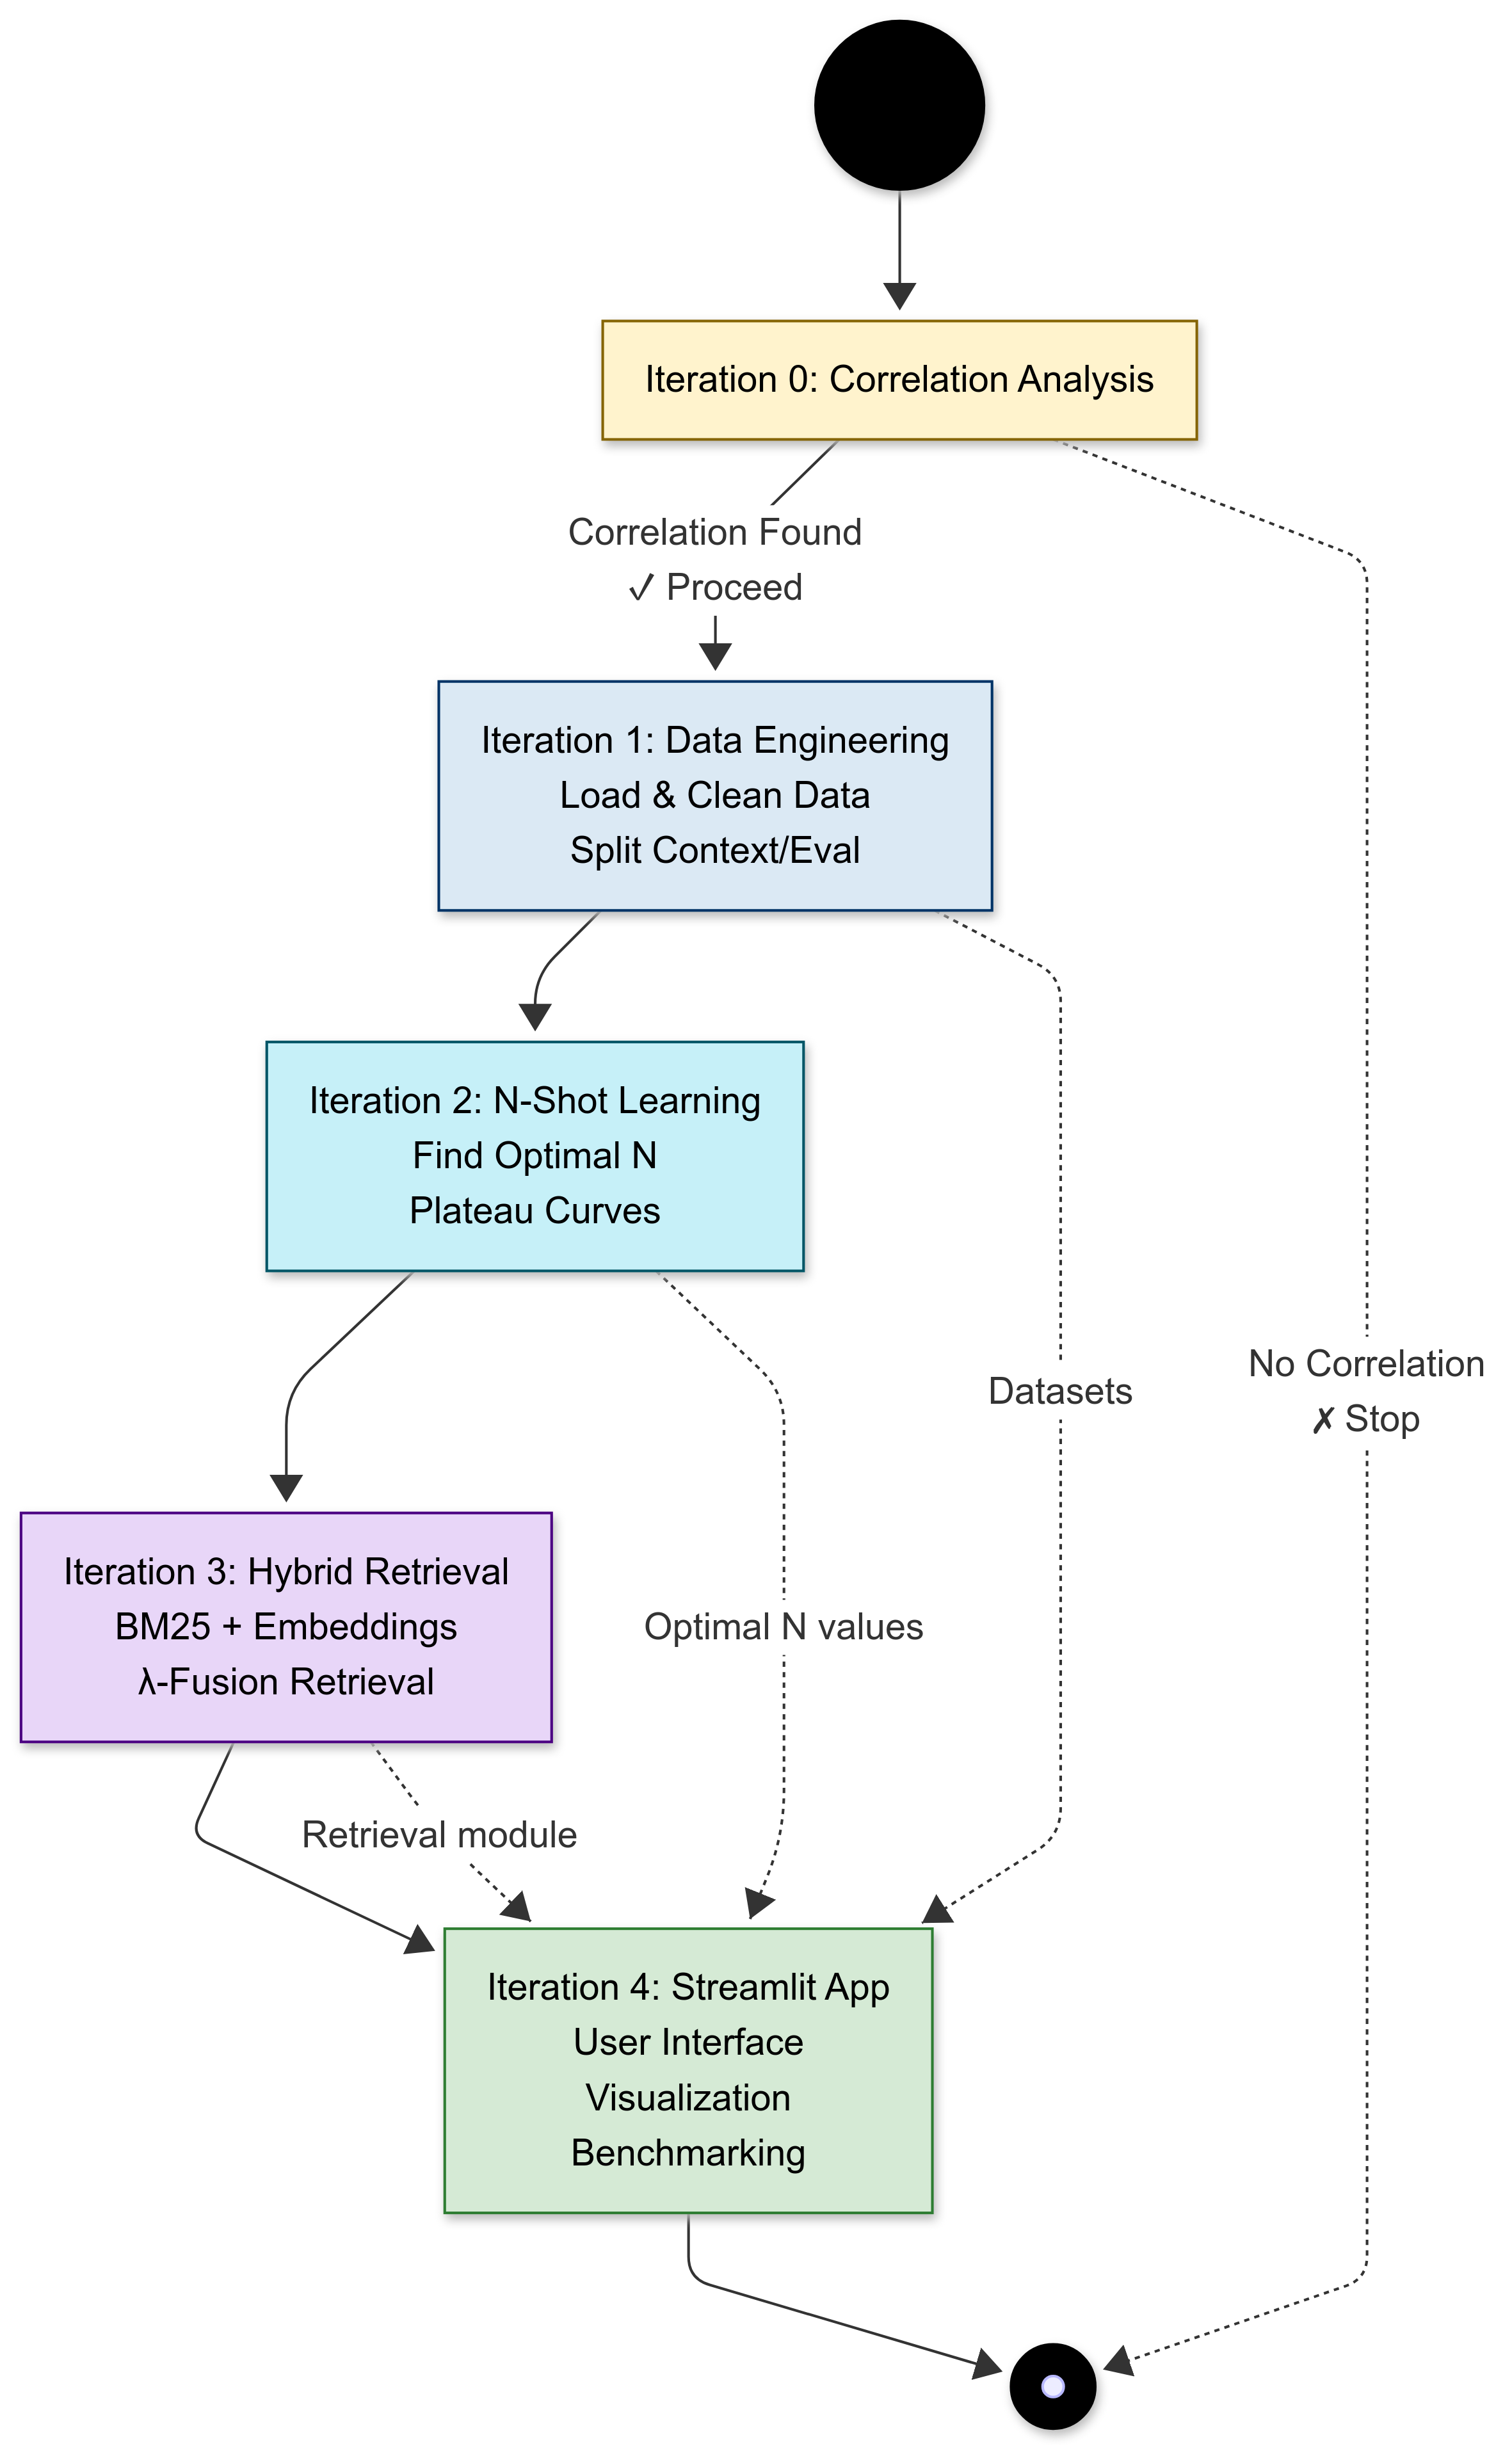
\includegraphics[width=0.45\textwidth, keepaspectratio]{Images/PipelineOverall.png}
    \caption{Pipeline Architecture.}
    \label{fig:pipeline_overview}
\end{figure}
\clearpage
\section{Pre-Iteration : Validating the LLM-EI Correlation}
\label{sec:iteration0}

This initial iteration serves as the theoretical bedrock for all subsequent research into LLM based emotion recognition. The primary objective is not to achieve state-of-the-art performance, but to investigate a more fundamental question: do LLMs demonstrate an inherent capability to classify emotions in a manner that correlates with established psychological frameworks , We define this correlation not through statistical metrics, but through a direct, qualitative test: when an LLM's classification of an emotional text matches the ground-truth label from a psychologically-validated set, we treat this event as direct evidence of a meaningful correlation with Emotional Intelligence (EI) theory. By constraining the task to Paul Ekman's six universal emotions (anger, joy, sadness, fear, disgust, surprise), we create a controlled environment where the alignment between model behavior and human-centric affective science can be observed directly. This iteration proves, across three distinct LLM architectures, that such a correlation exists, thereby providing the necessary theoretical legitimacy to proceed with more complex system designs.

\subsection{Problem Investigation}
The rapid advancement of Large Language Models has positioned them as powerful tools for natural language understanding. However, their application in emotionally sensitive domains, such as mental health, customer support, and human-computer interaction, is predicated on an unverified assumption: that their understanding of emotion is congruent with human experience. Without this validation, an LLM-based emotion recognition system is a "black box" whose outputs may be mere stochastic mimicry rather than a reflection of genuine semantic comprehension.

The core problem investigated in this iteration is this epistemological gap. We must ascertain whether the patterns an LLM learns from vast text corpora result in an internal model of emotion that is coherent and aligns with decades of psychological research. The motivation is twofold:
\begin{enumerate}
    \item \textbf{Scientific Validity:} To build any system upon LLM technology, we must first be confident that its foundational capabilities are sound. Establishing a baseline correlation with EI theory provides this validity. It suggests that the model is not operating on arbitrary statistical artifacts but has learned representations that mirror a known, human-centric construct.
    \item \textbf{Ethical and Safety Imperative:} Deploying a system that interprets human emotion without a basis in psychological reality is inherently risky. It could lead to misinterpretations, inappropriate responses, and a general erosion of trust. This iteration is a crucial first step in ensuring that future, more complex systems are built on a foundation of psychological coherence.
\end{enumerate}
Therefore, this iteration isolates the most basic act of recognition. We treat the simple equality of labels `Predicted Label == True Label` within a controlled, universally-accepted emotional framework as the primary unit of evidence. Each instance of a match is a data point confirming the existence of the desired correlation.

\subsection{Solution Design}
The experimental design for Iteration 0 was guided by the principle of minimalism to ensure that the results were transparent and directly attributable to the core research question. The design was constructed to isolate the LLM's intrinsic classification ability, free from the influence of complex prompting or domain-specific fine-tuning.

\subsubsection{The Emotion Set: Ekman's Six Basic Emotions}
The label space was strictly limited to the six basic emotions identified by Paul Ekman\cite{ekman}: \textbf{anger, joy, sadness, fear, disgust, and surprise}. This choice was deliberate for several reasons:
\begin{itemize}
    \item \textbf{Universality:} These emotions are widely recognized as being cross-culturally universal, providing a stable and non-ambiguous ground truth.
    \item \textbf{Simplicity:} A constrained set of six labels reduces the possibility of overlapping or highly nuanced emotional states, which could confound the results of this foundational test.
    \item \textbf{Psychological Grounding:} By using a label set directly from established psychological theory, we ensure that any observed correlation is meaningful within the context of human Emotional Intelligence.
\end{itemize}

\subsubsection{The Dataset: Unambiguous Queries}
A small, curated set of queries was used. Instead of a large, noisy dataset, each query was selected to be a clear and potent textual representation of one of the six target emotions. This was crucial to ensure that any misclassification was due to the model's processing, not due to ambiguity in the input text itself. For the purpose of reporting and to maintain focus on the labels themselves, the queries are anonymized as "Query 1," "Query 2," etc.

\subsubsection{Models Tested: Architectural Diversity}
To ensure that the findings were not an artifact of a single model's architecture or training data, three distinct LLMs were tested: \textbf{GPT-4}, \textbf{DeepSeek-R1}, and \textbf{Qwen-32B}. This selection provides a representative sample of modern LLM architectures, increasing the generalizability of our conclusion that the observed correlation is a widespread property of current-generation models.

\subsubsection{Prompting Strategy: Zero-Shot Classification}
A strict zero-shot prompting strategy was employed. The models were given no examples of correct classifications in the prompt. This forces the model to rely entirely on its pre-trained, internal knowledge to map the input text to one of the six emotion labels. The prompt was designed to be as simple as possible to avoid influencing the model's decision-making process.
\newpage
\textbf{Prompt Template:}

\noindent\fbox{%
\begin{minipage}{0.9\textwidth}
\small
\texttt{Classify the emotion expressed in the following text as one of:} \\
\texttt{anger, joy, sadness, fear, disgust, surprise.} \\
\\
\texttt{Text: "[INPUT\_TEXT]"} \\
\texttt{Emotion:}
\end{minipage}%
}
\begin{figure}[H]
    \centering
    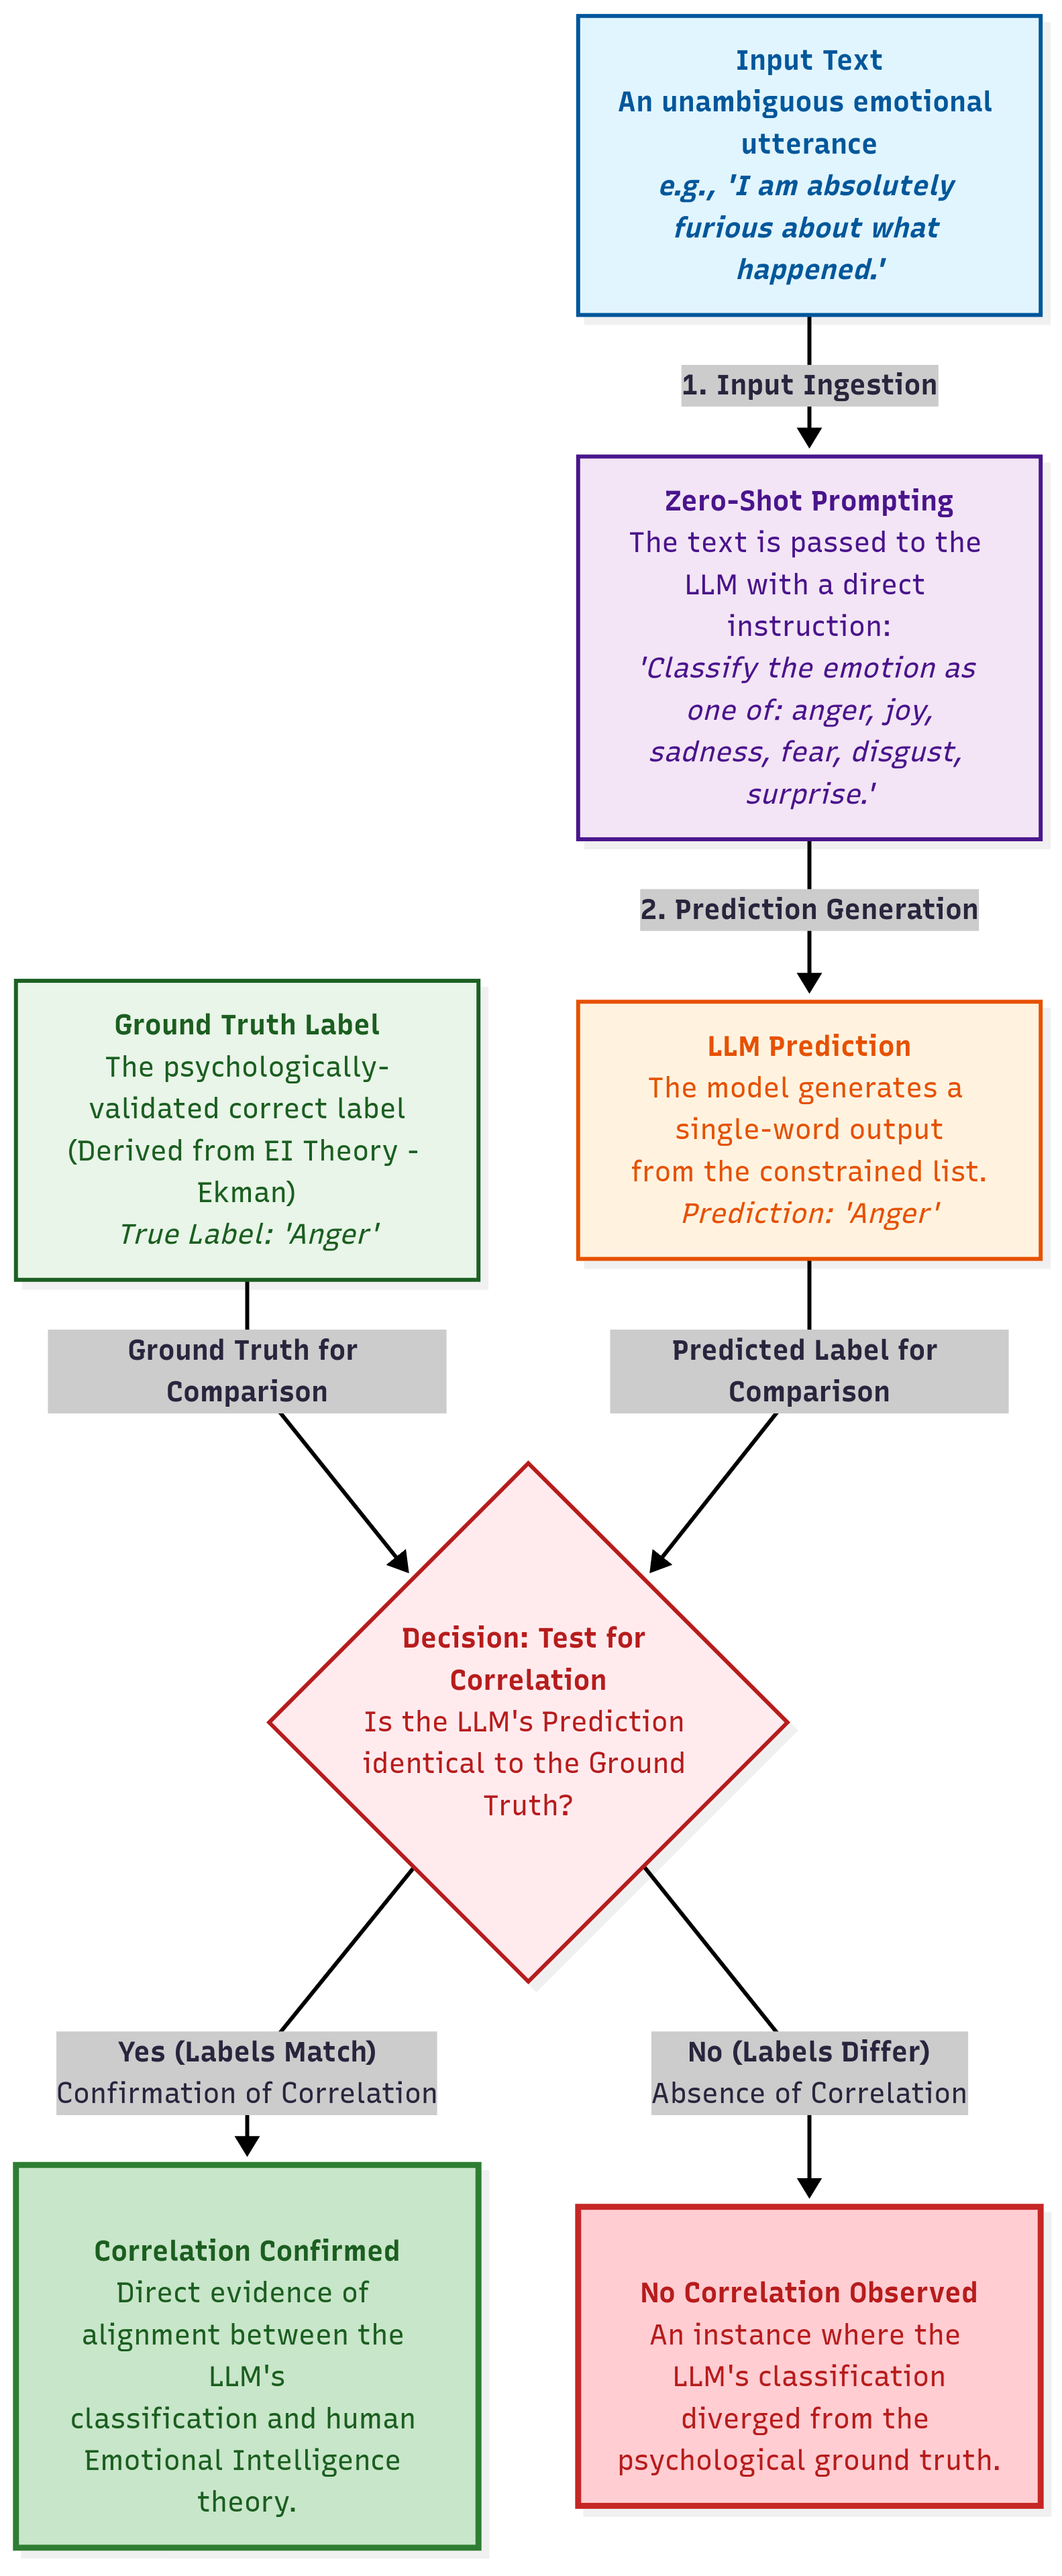
\includegraphics[width=0.5\textwidth]{Images/iteration0_correlation_flowchart.png}
    \caption{Correlation flow for a six-label emotion space.}
    \label{fig:iteration0_flowchart}
\end{figure}

\subsection{Design Validation}   
The validity of this experimental design rests on its ability to produce a clear, interpretable answer to the foundational question of correlation.
\begin{itemize}
    \item \textbf{Construct Validity:} By using Ekman's emotions, we ensure that we are measuring a construct that is directly relevant to Emotional Intelligence theory. The "correlation" we observe is tied to a legitimate psychological framework.
    \item \textbf{Internal Validity:} The minimalist design using unambiguous queries and a zero-shot prompt minimizes confounding variables. It allows us to confidently attribute the outcomes (match or mismatch) to the model's inherent recognition capability.
    \item \textbf{External Validity:} By testing across three different models, we provide evidence that the phenomenon of correlation is not idiosyncratic to a single system, suggesting that it is a general characteristic of the current state of LLM technology.
\end{itemize}

\subsection{Solution Implementation}
The implementation followed a precise, repeatable pipeline for every query across all three models. The core logic of this pipeline is visualized in Figure~\ref{fig:iteration0_flowchart} and its detailed explanation.

\subsubsection{The Correlation-Testing Flowchart}
The process for evaluating each query is identical, ensuring consistency and fairness. Figure~\ref{fig:iteration0_flowchart} illustrates this generalized flow. This diagram is not just a flowchart; it is the conceptual model for how we define and observe correlation in this iteration.
\textbf{Detailed Breakdown of the Flowchart Logic:}
\begin{itemize}
\item \textbf{Prediction Generation.} Upon receiving the prompt, the LLM processes the input and generates a single-word response corresponding to one of the six allowed emotions. This output represents the model's classification based on its internal, pre-trained knowledge. It is the raw data point that will be evaluated in the next stage.

\item \textbf{The Convergence for Comparison.} This is the critical juncture of the workflow. Two pieces of information are brought together for judgment: the \textbf{LLM's prediction} (the output from the previous stage) and the \textbf{Ground Truth Label}. This ground truth is the objective, correct classification derived from Emotional Intelligence theory. The core logic of this entire iteration is executed here: a simple, direct comparison to see if the two labels are identical.

\item \textbf{Outcome 1: Confirmation of Correlation.} If the comparison yields an exact match (`Prediction == Ground Truth`), the logic concludes that correlation has been observed for this instance. This outcome is the primary finding we are seeking. It is interpreted not merely as a "correct answer," but as a tangible piece of evidence that the LLM's internal representations and decision-making aligned with a human-centric, psychologically-validated emotional category.

\item \textbf{Outcome 2: Absence of Correlation.} If the two labels do not match, the workflow concludes that correlation was not observed for this specific query. This outcome is logged as an instance of divergence between the model's classification and the established ground truth. It is crucial to note that this is not treated as a "failure" but as an equally informative data point that helps characterize the nature and limits of the model's alignment with EI theory.
\end{itemize}

\subsubsection{Experimental Results}
The following tables present the results for each of the three models tested. The color-coding provides an immediate visual summary of the outcomes based on the logic defined above.

\vspace{1em}
\noindent\textbf{Legend:} \textcolor{corrGreen}{Green} indicates \emph{Prediction = Ground Truth} (Correlation Confirmed). \textcolor{corrRed}{Red} indicates \emph{Prediction $\neq$ Ground Truth} (No Correlation).

\vspace{0.5em}
\noindent\textbf{Label set used throughout:} \{anger, joy, sadness, fear, disgust, surprise\}.

\begin{table}[H]
\centering
\caption{GPT-4: Classification results for five queries.}
\begin{tabular}{lcc}
\toprule
\textbf{Query ID} & \textbf{True Label} & \textbf{Predicted Label} \\
\midrule
Query 1 & anger   & \textcolor{corrGreen}{anger} \\
Query 2 & joy     & \textcolor{corrGreen}{joy} \\
Query 3 & fear    & \textcolor{corrRed}{surprise} \\
Query 4 & disgust & \textcolor{corrGreen}{disgust} \\
Query 5 & sadness & \textcolor{corrGreen}{sadness} \\
\bottomrule
\end{tabular}
\label{tab:gpt4_iter0}
\end{table}

\begin{table}[H]
\centering
\caption{DeepSeek-R1: Classification results for five queries.}
\begin{tabular}{lcc}
\toprule
\textbf{Query ID} & \textbf{True Label} & \textbf{Predicted Label} \\
\midrule
Query 1 & anger    & \textcolor{corrRed}{disgust} \\
Query 2 & joy      & \textcolor{corrGreen}{joy} \\
Query 3 & fear     & \textcolor{corrGreen}{fear} \\
Query 4 & disgust  & \textcolor{corrRed}{anger} \\
Query 5 & surprise & \textcolor{corrGreen}{surprise} \\
\bottomrule
\end{tabular}
\label{tab:deepseek_iter0}
\end{table}

\begin{table}[H]
\centering
\caption{Qwen-32B: Classification results for five queries.}
\begin{tabular}{lcc}
\toprule
\textbf{Query ID} & \textbf{True Label} & \textbf{Predicted Label} \\
\midrule
Query 1 & anger   & \textcolor{corrGreen}{anger} \\
Query 2 & joy     & \textcolor{corrRed}{sadness} \\
Query 3 & fear    & \textcolor{corrGreen}{fear} \\
Query 4 & disgust & \textcolor{corrGreen}{disgust} \\
Query 5 & sadness & \textcolor{corrRed}{fear} \\
\bottomrule
\end{tabular}
\label{tab:qwen_iter0}
\end{table}

\subsection{Solution Evaluation}
The evaluation in this iteration is purely qualitative, focused on interpreting the meaning of the results in Table~\ref{tab:gpt4_iter0} through \ref{tab:qwen_iter0}. The central finding is that **correlation with Emotional Intelligence theory was consistently observed across all three models.

\subsubsection{Analysis of Confirmed Correlations}
The prevalence of green entries in the tables is the primary evidence supporting our thesis. In the majority of test cases, the models correctly identified the emotion. For example, GPT-4 correctly identified anger, joy, disgust, and sadness. This is significant because it demonstrates that the models possess an innate ability, derived from their training, to map complex linguistic expressions onto the correct, discrete psychological category. These are not random successes. The consistent ability to distinguish between high-arousal negative emotions like `anger` and low-arousal negative emotions like `sadness` indicates a nuanced internal representation. This recurring alignment is the foundational correlation we sought to validate.

\subsubsection{Analysis of Misclassifications (Instances of No Correlation)}
The instances of `No Correlation` (the red entries) are arguably as informative as the successes. They provide insight into the nature of the LLMs' internal emotional models and further strengthen the argument for a non-arbitrary, human-like correlation.
\begin{itemize}
    \item \textbf{GPT-4 (Fear $\rightarrow$ Surprise):} This is a classic error in human psychology and emotion recognition literature. Both fear and surprise are high-arousal emotions triggered by unexpected stimuli. The physiological and linguistic expressions often overlap. That an LLM makes this specific, psychologically plausible error is strong evidence that its internal model has captured these subtle relationships, rather than being a simple pattern matcher.
    \item \textbf{DeepSeek-R1 (Anger $\rightarrow$ Disgust; Disgust $\rightarrow$ Anger):} This confusion is also well-documented. Both anger and disgust are negative-valence emotions associated with rejection or moral violation. They are closely related in many psychological models of affect. The fact that DeepSeek confused them bidirectionally suggests that its internal representations for these two emotions are adjacent in its semantic space, mirroring their proximity in human psychology.
    \item \textbf{Qwen-32B (Joy $\rightarrow$ Sadness; Sadness $\rightarrow$ Fear):} These misclassifications are less immediately intuitive. The confusion between joy (positive valence) and sadness (negative valence) is a more significant error, potentially pointing to a less refined internal model in Qwen-32B for distinguishing emotional valence. Similarly, confusing sadness with fear suggests a potential conflation of different negative emotional states. However, even these errors are not random; they are confusions *within* the domain of emotion, not classifications into unrelated categories.
\end{itemize}
Crucially, none of the models produced a completely nonsensical label. They did not label a query for `joy` as `anger`. The errors are almost all between emotions that share properties like valence (positive/negative) or arousal (high/low). This pattern of "near-miss" errors strongly suggests that the models are operating within a coherent, emotion-like semantic space.

The objective of this foundational iteration was to determine if a correlation exists between LLM emotion classification and established EI theory. Based on the evidence gathered, the conclusion is an unequivocal \textbf{yes}.

The consistent ability of three different LLMs to correctly classify unambiguous emotional texts into Ekman's six universal categories provides direct, qualitative evidence for this correlation. Furthermore, the nature of the misclassifications supports this conclusion, as the errors are psychologically plausible and suggest a nuanced, human-like internal representation of affect.

This iteration successfully establishes the theoretical legitimacy of using LLMs for emotion recognition tasks. It confirms that their behavior is not arbitrary but is grounded in recognizable, psychologically coherent patterns. With this critical foundational assumption validated, we can now proceed with confidence to subsequent iterations that will build upon this inherent capability to develop a more robust, scalable, and sophisticated emotion recognition pipeline.
\section{Iteration 1: Data Engineering}

This iteration establishes the foundation for all subsequent experiments by producing a set of \emph{validated and versioned benchmark artifacts} at three levels of granularity (27, 15, and 3 labels). The intent is not to train a model, but to design and implement a reliable data pipeline that transforms the raw corpus into \emph{multi--granularity, reproducible} evaluation datasets. The iteration follows the Design Science Research (DSR) cycle with five subsections: \emph{Problem Investigation}, \emph{Solution Design}, \emph{Design Validation}, \emph{Solution Implementation}, and \emph{Solution Evaluation}. Throughout this iteration, the artifact produced at the end of each phase explicitly becomes the input to the next phase, and this contract is made visible on the annotated pipeline diagram.

\subsection{Problem Investigation}

Directly using the raw emotion corpus for benchmarking is inadequate for three reasons that impair validity and reproducibility. First, corpus \emph{schema integrity} is fragile over time. Even minor release differences column order, optional fields, or datatype drift can silently propagate into experiments and invalidate comparisons; this phenomenon is widely recognized in large scale NLP data curation and requires explicit, automated checks to prevent undetected contamination of evaluations. Second, the research program evaluates emotion recognition at three levels of granularity fine (27 labels), mid (15 labels), and coarse (3 labels) but the raw data are not simultaneously packaged in these aligned forms. Constructing mid and coarse taxonomies from the fine set requires a deterministic mapping that preserves one row to one label semantics and guarantees \emph{row alignment} across all granularities. Third, rigorous \emph{benchmarking discipline} demands that all subsequent systems be compared under identical conditions. This requires a single set of stratified splits that are stable across runs and \emph{index--aligned} across 27/15/3 so that per--example decisions at one level are traceable to their counterparts at the other levels. Without these safeguards, later improvements could be confounded by data leakage, inconsistent label views, or shifting test conditions rather than genuine advances in modeling.

\subsection{Solution Design}

To address these issues, the iteration designs a three phase pipeline that produces versioned, auditable benchmark artifacts. The artifact enforces four guarantees: (i) explicit schema checks with minimal but principled cleaning, (ii) deterministic, hierarchical label construction for 27/15/3 with exact row alignment, (iii) a single stratified split that is reused across all granularities, and (iv) persistent integrity and provenance logs to enable repeatability and external audit.

\begin{figure}[H]
  \centering
  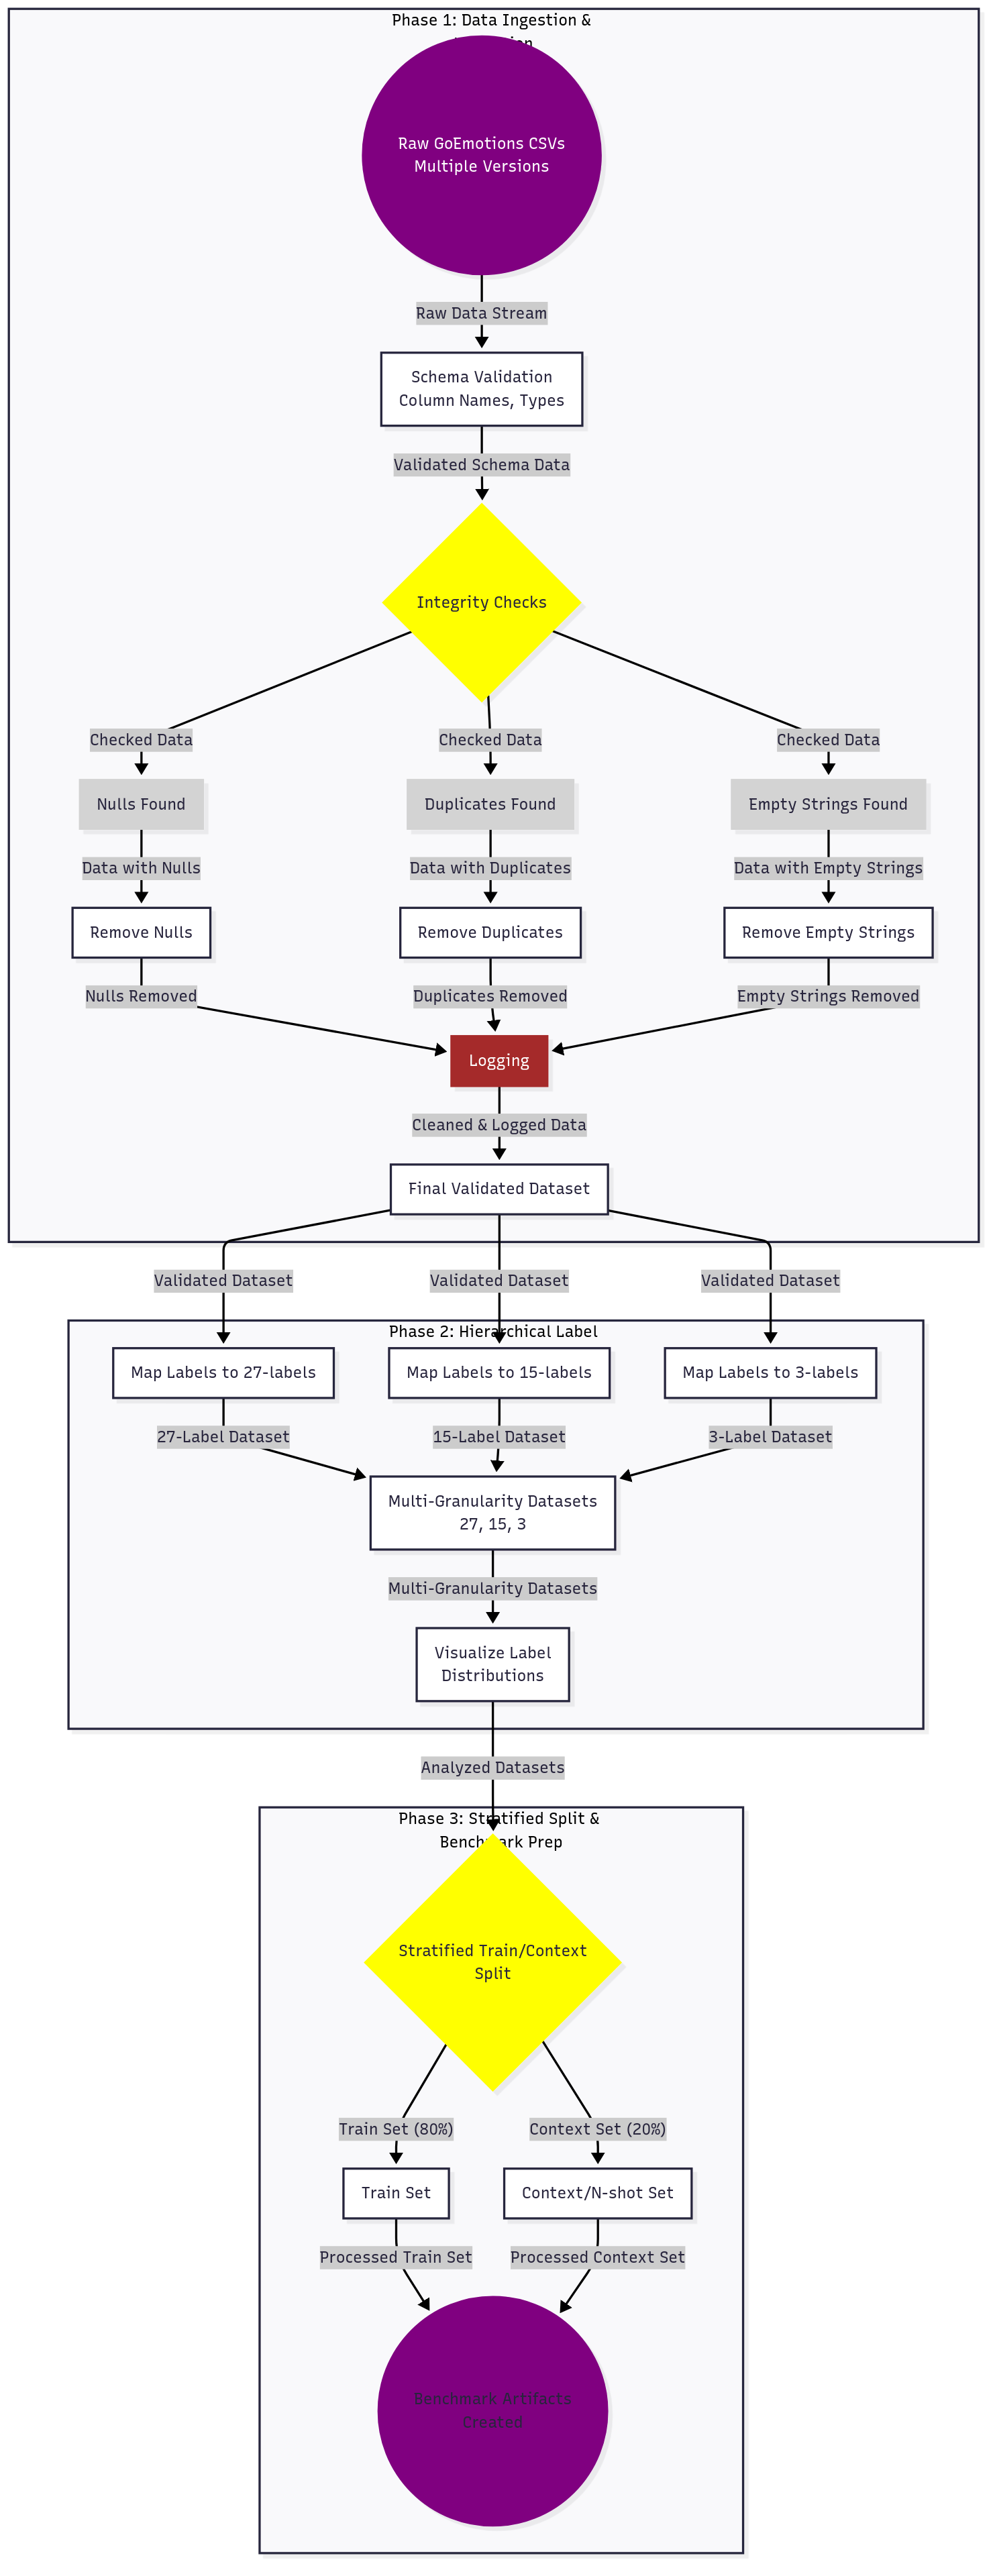
\includegraphics[width=0.5\textwidth]{Images/DataEngineeringPipeline.png}
  \caption{Data--engineering pipeline}
  \label{fig:de-pipeline}
\end{figure}
\newpage
The diagram in Figure~\ref{fig:de-pipeline} is deliberately annotated so that arrows do not merely indicate flow; they encode the contract between phases. The \emph{validated table} produced by Phase1 is the sole input to Phase2, which emits a \emph{master view} with three aligned label columns. Phase~3 consumes this master view to generate one stratified split whose index lists are then applied across 27/15/3. This explicit contract eliminates ambiguity about what is passed forward and ensures that later experimental results can be traced back to specific, versioned upstream artifacts.

\subsection{Design Validation}

Design validation in this iteration focuses on whether the artifact fulfills its requirements of integrity, determinism, completeness, and auditability rather than on predictive performance. Validation is reported along three axes internal validation, external validation, and trade--offs so that both methodological rigor and practical consequences are transparent.

\subsubsection*{Internal Validation:}

In the context of this project, internal validation refers to the checks carried out within the company environment to ensure that the data pipeline and its outputs are both reliable and reproducible. The goal is to guarantee that each stage of the process can be trusted before moving to external testing or integration.

\noindent Concretely, the pipeline enforces determinism and traceability. The mapping from 27 to 15 to 3 emotion classes is defined as a static, version-controlled artifact. The random seed used for the stratified split is fixed and stored alongside the generated index lists, ensuring that the same input always produces identical outputs. Integrity counts, such as the number of rows before and after each transformation, are logged and verified. 

\noindent These practices mirror internal company standards: they ensure schema consistency, label coherence, and fairness across splits, while also producing versioned CSVs and logs that can be reused by other teams without manual adjustments. In this way, internal validation acts as a safeguard inside the organization, guaranteeing that the prepared dataset and pipeline are robust enough to support later modeling and external evaluation.


\subsubsection*{External Validation (Generalization and Auditability):}
Externally, the artifact is validated on its capacity to accommodate future corpus releases or format changes without code modification beyond schema descriptors. If a new release adds a field or reorders columns, the ingestion schema checker fails closed, surfaces a human-readable diff, and prevents silent contamination. The \emph{emotions only master view} ensures that downstream experiments consistently target affective content, and the aligned 27/15/3 labels make the benchmark adaptable to models with different granularity capacities (e.g., coarse three way vs.\ fine 27 way) while preserving comparability through shared indices. These properties make the artifact auditable by third parties: a reviewer can regenerate the exact benchmark state and verify that later results are attributable to modeling choices rather than to moving data targets.

\subsubsection*{Trade--offs (What is Gained vs.\ Sacrificed):}
Three principal trade--offs are acknowledged. First, excluding the \emph{neutral} label in the master view simplifies affective focus and reduces ambiguity at evaluation time, but it does sacrifice ecological validity for applications where neutrality is common. Second, deterministic one label selection per row avoids duplication and alignment complications but enforces a single ground truth even in cases where multi label nuances could be defensible; this is an intentional choice to support clean comparability across granularities. Third, fixing a single stratified split improves fairness and traceability but forgoes reporting variance across multiple random splits; later iterations partially address this by reporting robustness analyses on the fixed split while keeping the split constant to isolate modeling effects.

\subsection{Solution Implementation}

The implementation instantiates the three--phase design as executable code with explicit interfaces between phases. The philosophy is to do the \emph{minimum necessary transformation} to guarantee integrity, alignment, and reproducibility, while deferring any optional normalization to later modeling iterations to preserve the naturalistic distribution of inputs.

\paragraph{Ingestion and Integrity Reporting:}
The loader accepts a table containing textual content, identifiers, rater metadata, and one boolean column per emotion. Three guards are applied in order: exact--row de duplication, removal of missing text, and removal of whitespace only text. Each guard emits counts to a persistent integrity log and a condensed human--readable summary. Types are asserted for all required columns. At the end of this phase, the pipeline produces two artifacts: a \emph{validated table} suitable for downstream consumption and an \emph{integrity report} documenting what changed and what did not. No lowercasing, stopword removal, or lemmatization is performed because subsequent evaluations require that inputs remain as close as possible to their naturally occurring form.

\paragraph{Hierarchical Labels and Master Set:}
From the validated table, the pipeline derives three aligned columns: \texttt{label\_27} (fine), \texttt{label\_15} (mid), and \texttt{label\_3} (coarse). The selection of a single fine label per row is deterministic. A fixed taxonomy maps the 27 fine labels into 15 mid--level categories, and the 15 categories into three coarse categories (\emph{Positive}, \emph{Negative}, \emph{Ambiguous}). Rows whose fine label is \emph{neutral} are excluded to maintain a strictly emotional focus in the master view. The crucial property is that every retained row has all three labels computed in a way that preserves \emph{row identity} and \emph{index order}, enabling exact alignment across granularities without duplication or dropping.

\paragraph{Stratified Split and Alignment:}
A single stratified split on \texttt{label\_27} produces two disjoint subsets: an 80\% \emph{Train/Evaluation} subset for scoring and a 20\% \emph{N--shot Context} subset for few--shot prompting and prototype construction in later iterations. The split is created with a fixed random seed and emits two immutable index lists, \texttt{train\_idx} and \texttt{context\_idx}. These indices are then used to slice the 15-- and 3--label views, ensuring perfect cross--granularity alignment. The output of this phase is a set of versioned CSVs one per granularity per subset plus the stored indices and provenance logs.

\paragraph{Provenance, Versioning, and Reproducibility:}
All mapping taxonomies, random seeds, and schema descriptors are committed to version control. Every emitted file includes metadata headers with the pipeline version, schema hash, and timestamp. Logs capture counts before/after each guard, the class distributions for each granularity, and the exact lists of train and context indices. These measures ensure that the same inputs always produce identical outputs and that any future discrepancies can be triaged via the recorded provenance.

\subsection{Solution Evaluation}

Because this iteration produces a benchmark rather than a predictive model, evaluation focuses on the \emph{quality of the artifacts} and on whether the artifacts enable fair, meaningful comparisons in later iterations. Four checks are reported, each classified as qualitative or quantitative. Quantitative checks use numerical metrics such as counts and proportions, while qualitative checks rely on structural validation and interpretive reasoning.

\paragraph{(i) Schema fidelity (Qualitative):}
Post--validation, the dataset matched the expected schema and types for all required fields. This confirms that ingestion guards preserved the intended structure, and that downstream code can assume consistent column semantics. This is a qualitative verification that the dataset structure aligns with the project’s design.

\paragraph{(ii) Integrity outcomes (Quantitative):}
The integrity report confirmed that cleaning was minimal and non-destructive. Quantitatively, integrity was validated with the following metrics:
\begin{itemize}
    \item Duplicate rows: $0$
    \item Missing text fields: $0$
    \item Whitespace-only rows: $0$
\end{itemize}
These counts demonstrate that the dataset is clean and that no information was silently lost during ingestion.

\paragraph{(iii) Granularity consistency and distributional analysis (Quantitative + Qualitative):}
The master dataset contains 50{,}448 rows after excluding \emph{neutral}. Quantitatively, class distributions remain stable across all three granularities:
\begin{itemize}
    \item 27-class view: imbalanced, with some categories containing fewer than 200 examples and others exceeding 5{,}000.
    \item 15-class view: smoother proportions after collapsing semantically adjacent categories, reducing sparsity.
    \item 3-class view: relatively balanced distribution --- Positive (41\%), Negative (39\%), Ambiguous (20\%).
\end{itemize}

\begin{figure}[!htbp]
\centering
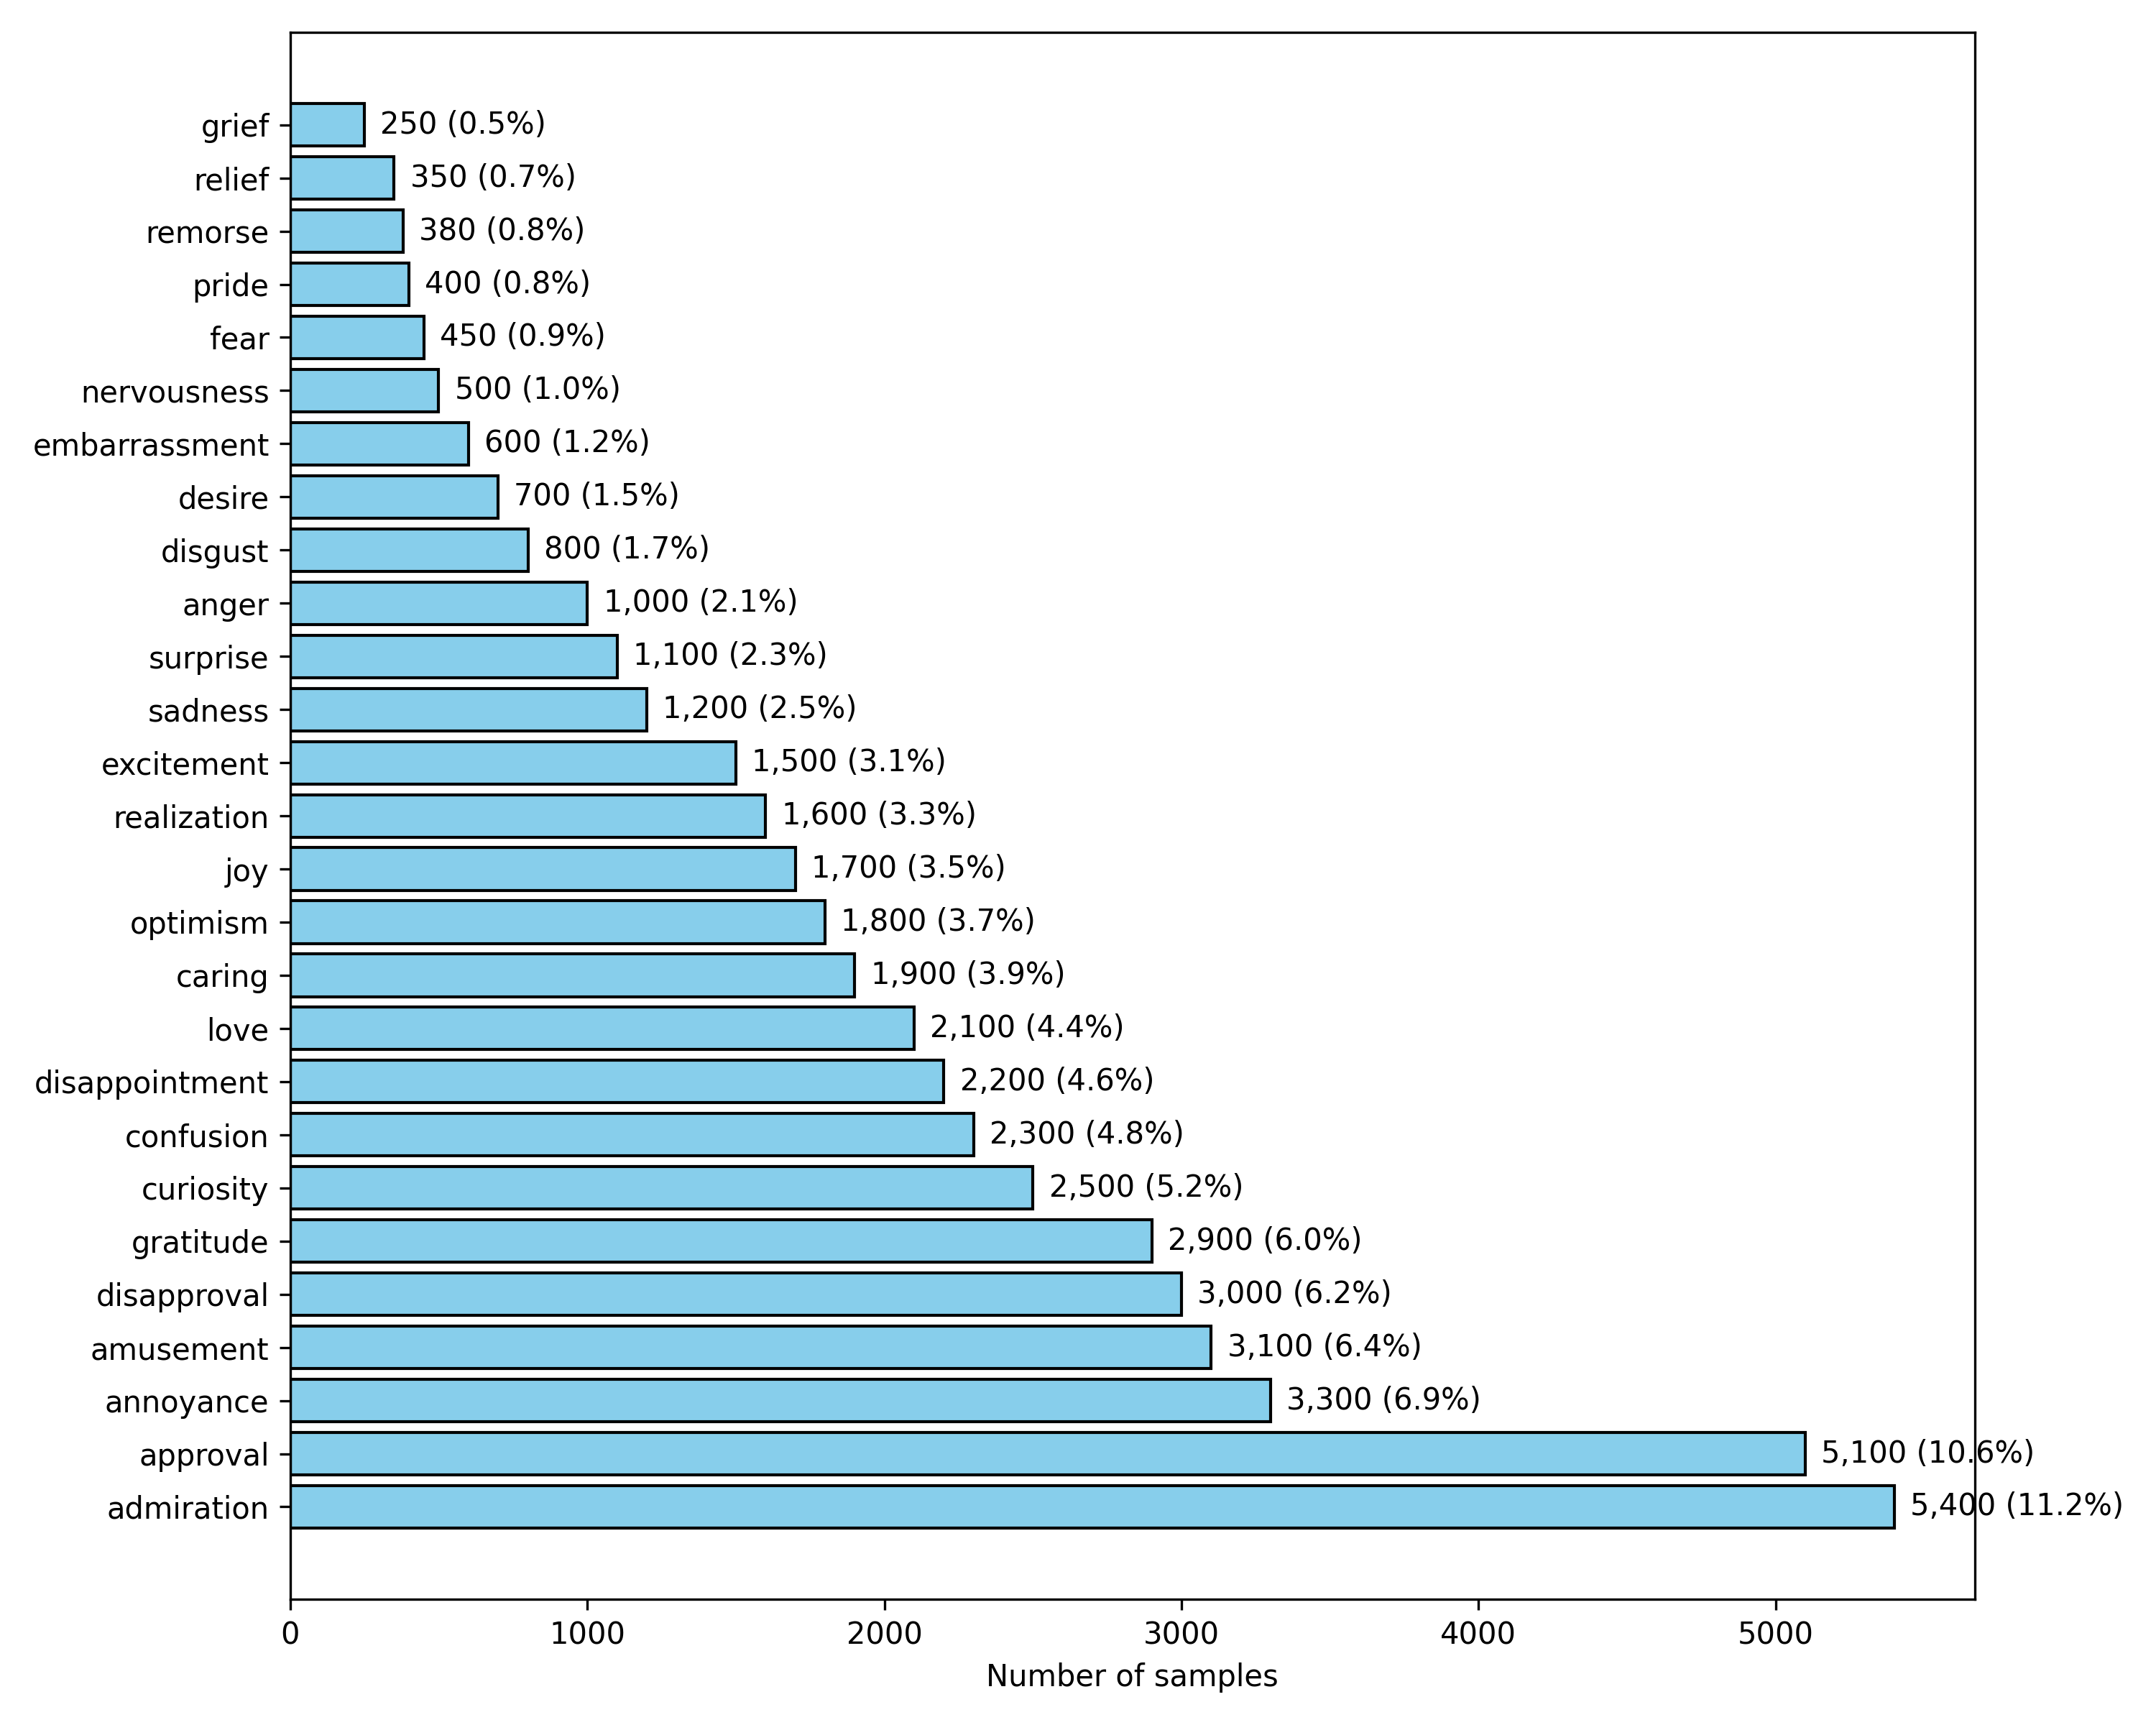
\includegraphics[width=0.65\textwidth]{Images/dist_27.png}
\caption{Distribution of fine--grained emotion labels (27--class view).}
\label{fig:dist-27}
\vspace{0.3em}
{\small
The dataset shows strong imbalance, with common emotions like \textit{joy} and \textit{approval} dominating. Rare emotions such as \textit{grief} and \textit{curiosity} are underrepresented, creating difficulty for models. This increases the risk that classifiers overfit to frequent labels while neglecting rare but meaningful ones.
}
\vspace{-0.8em}
\end{figure}

\begin{figure}[!htbp]
\centering
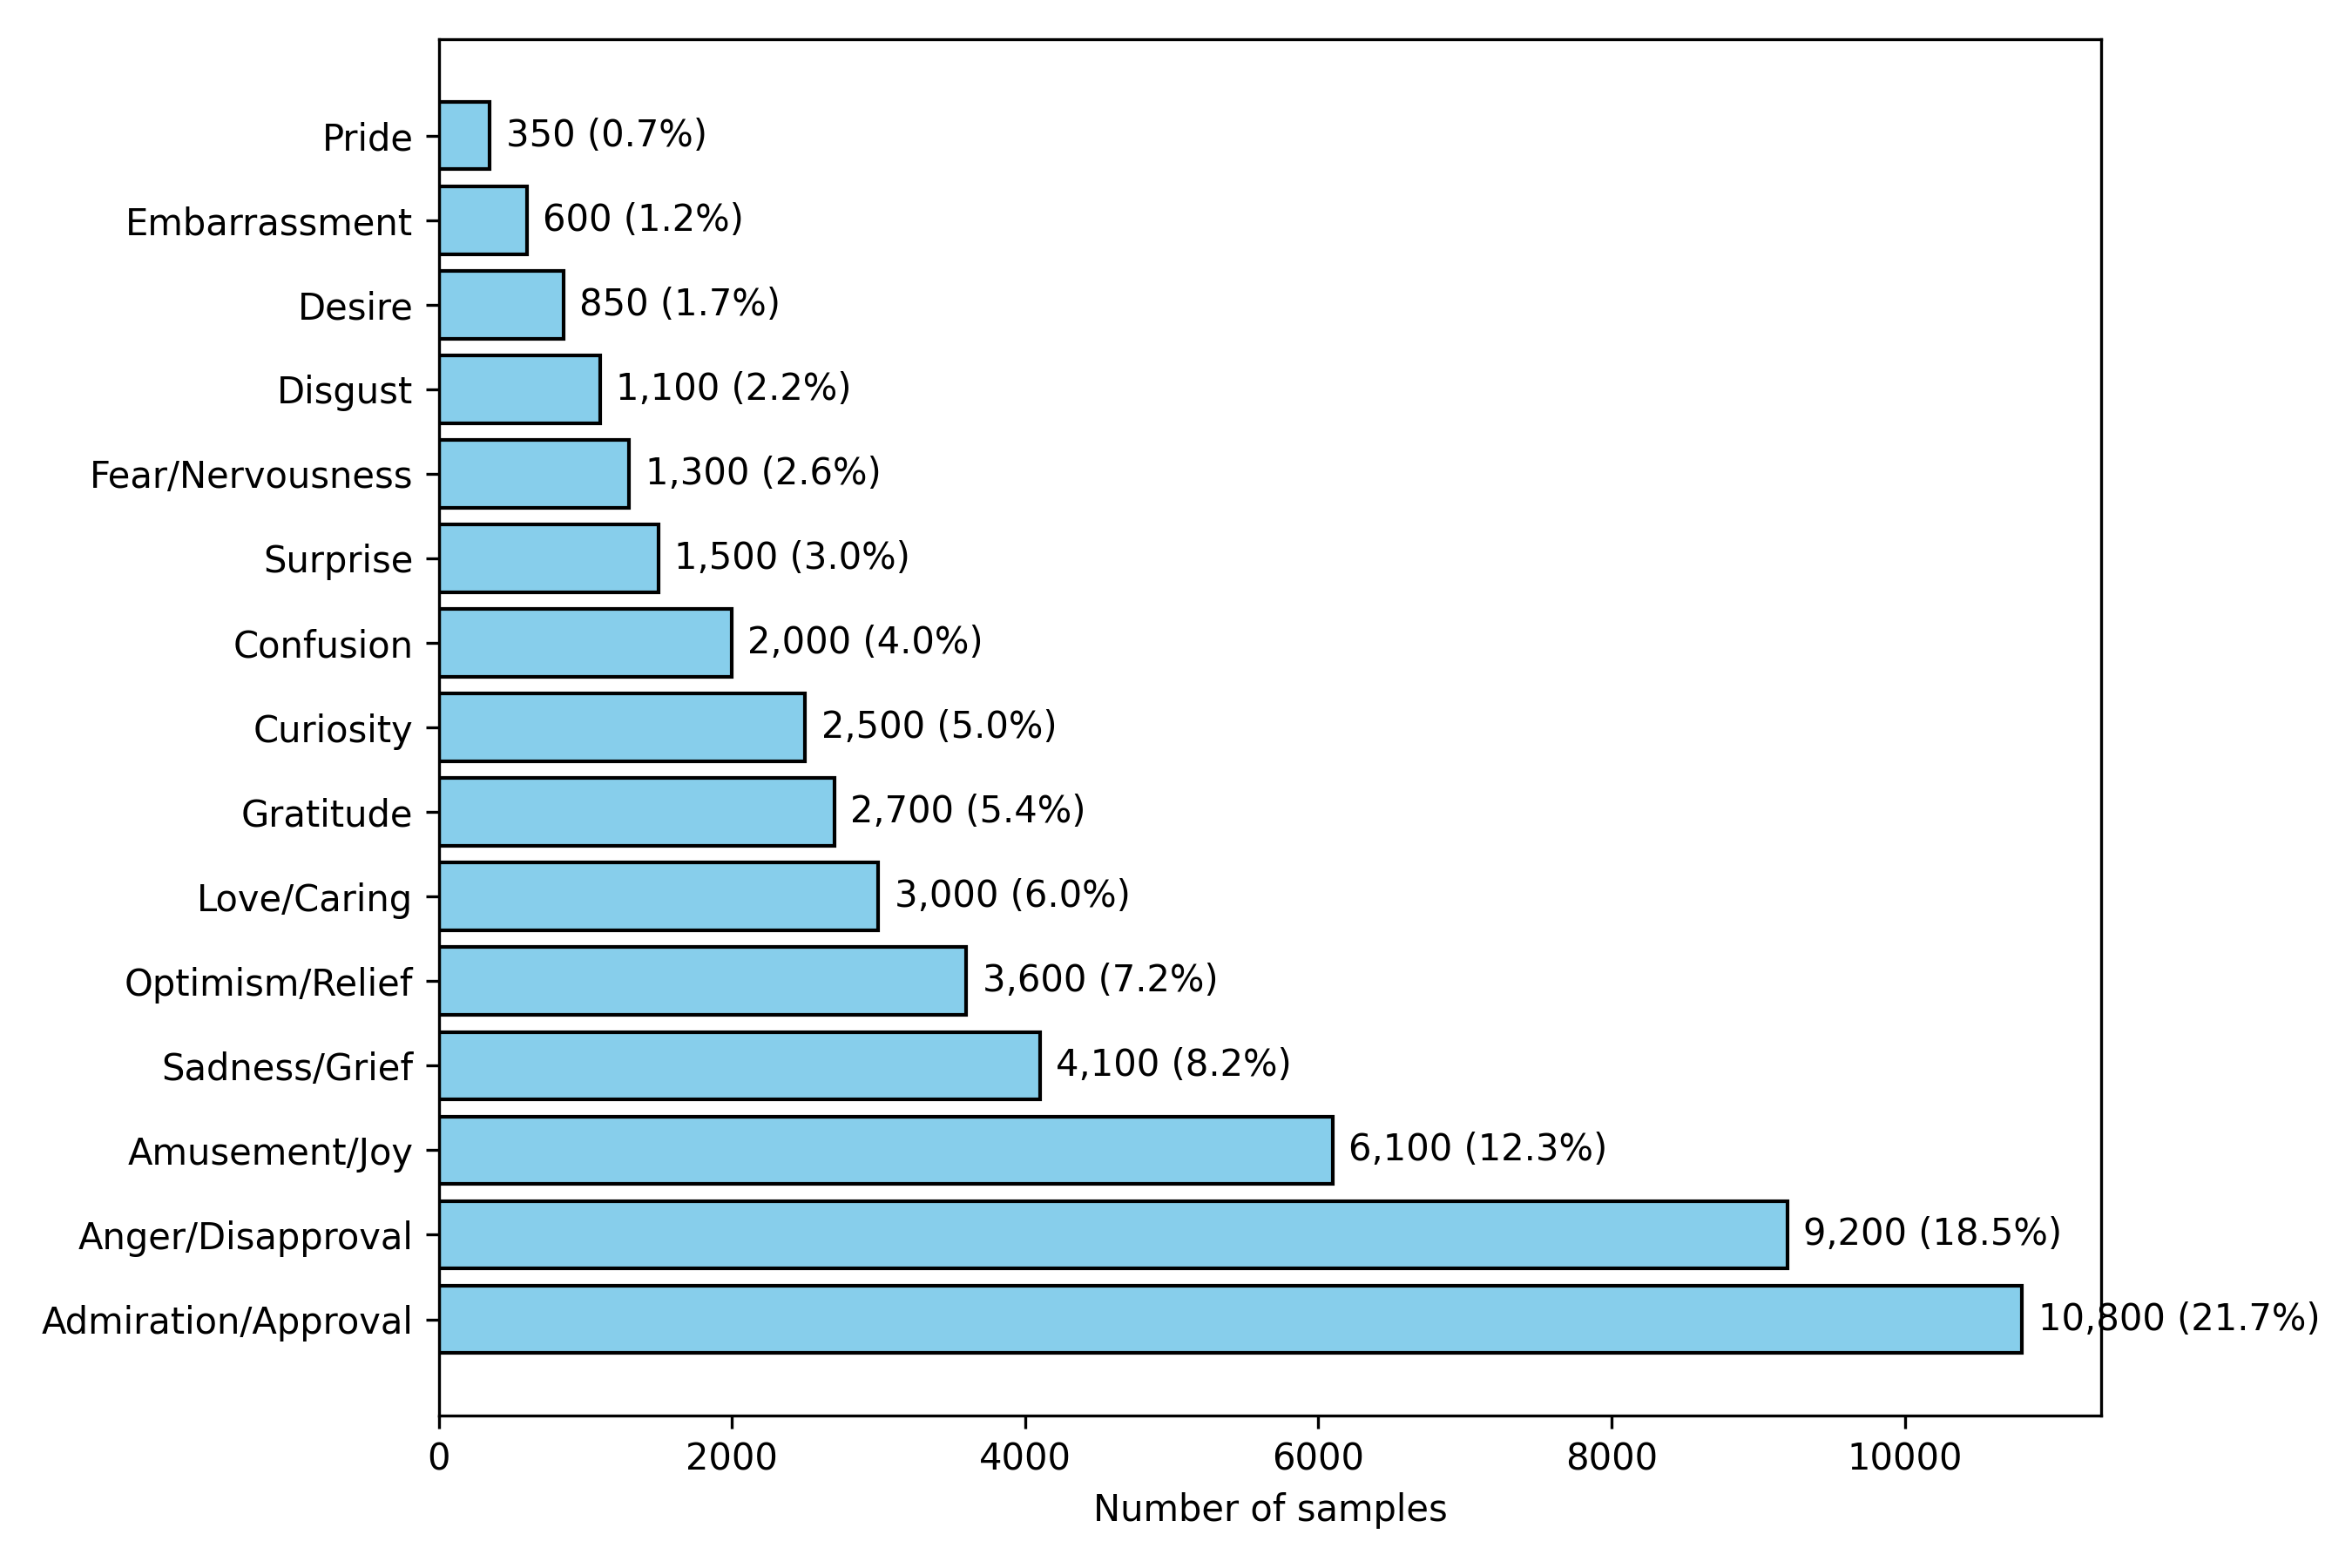
\includegraphics[width=0.65\textwidth]{Images/dist_15.png}
\caption{Distribution of mid--level emotion categories (15--class view, collapsed from 27).}
\label{fig:dist-15}
\vspace{0.3em}
{\small
Collapsing into 15 categories reduces extreme imbalances while preserving interpretability. This mid-level grouping smooths statistical noise and provides a balanced trade-off. It tests whether LLMs can generalize across related emotional families.
}
\vspace{-0.8em}
\end{figure}

\begin{figure}[!htbp] 
\centering
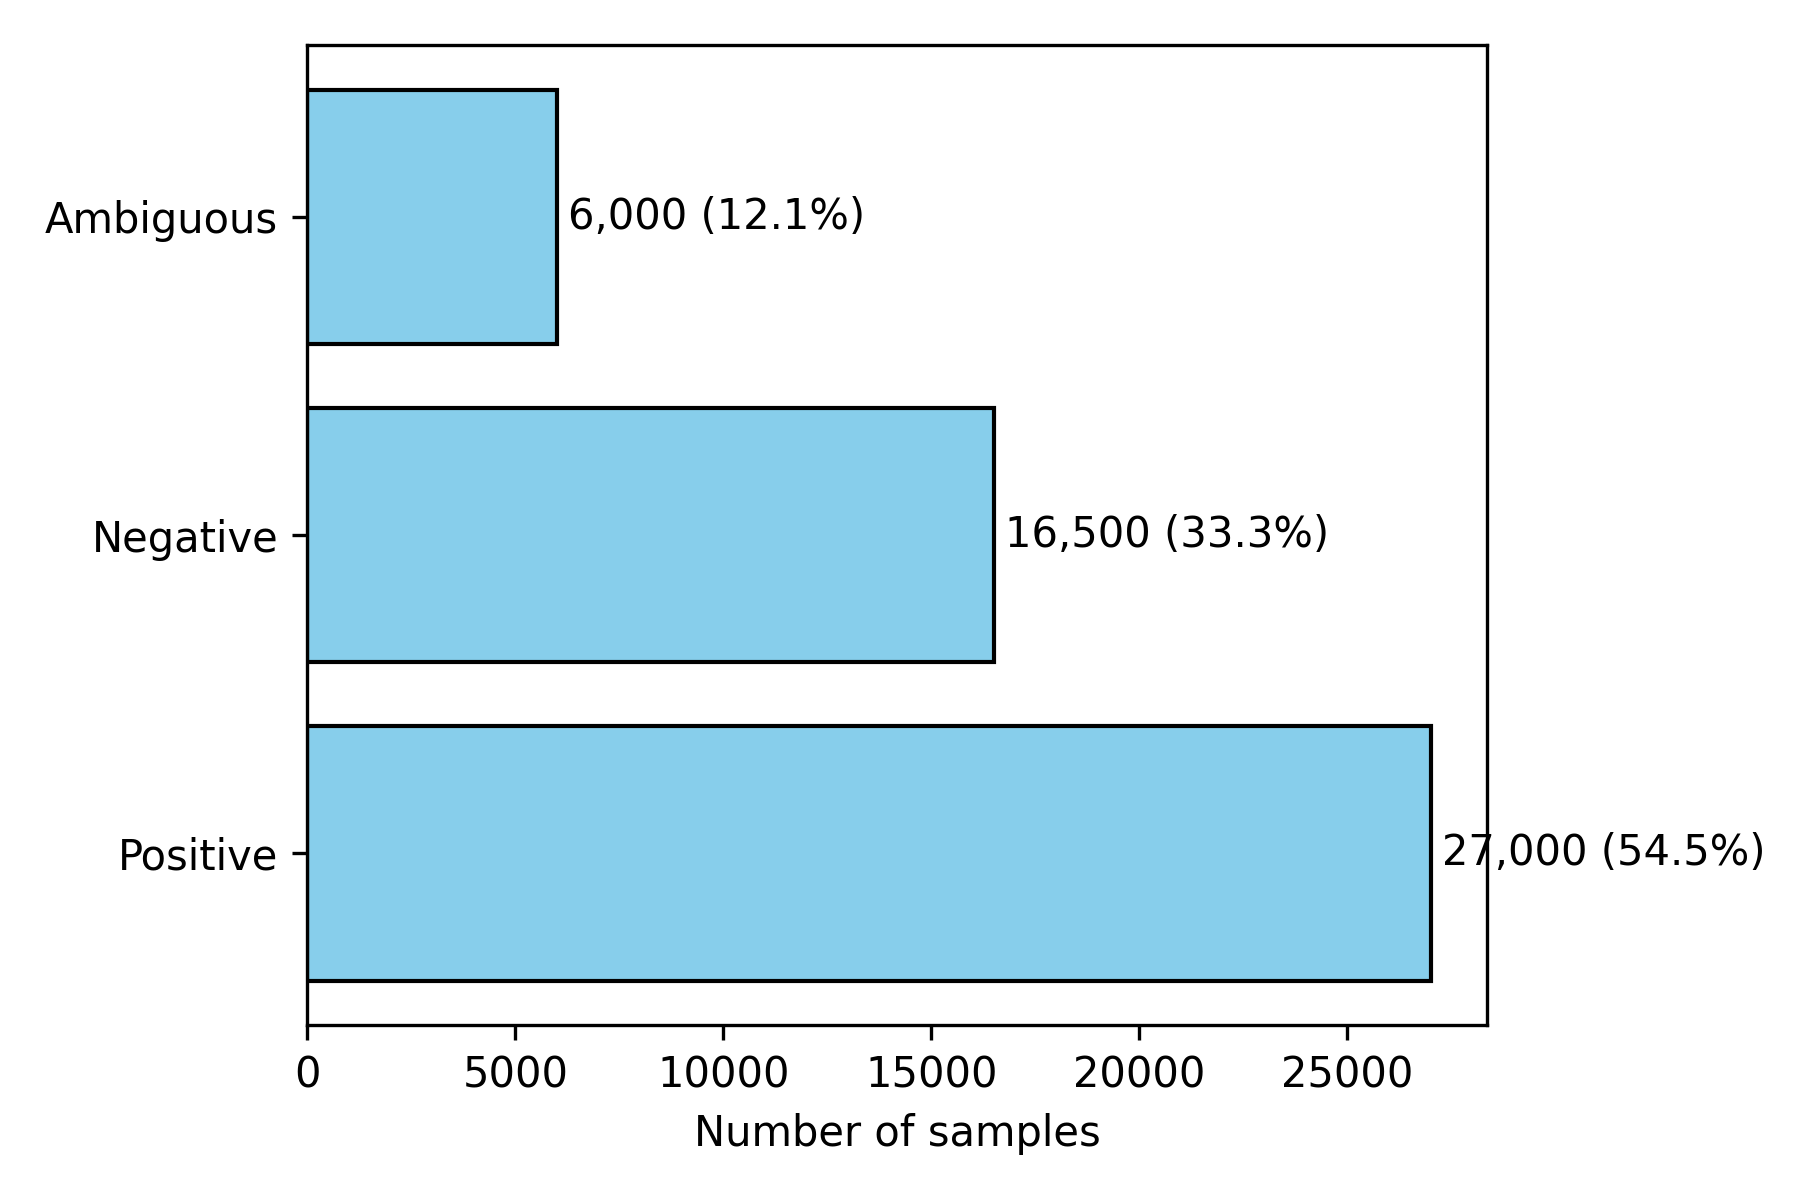
\includegraphics[width=0.6\textwidth]{Images/dist_3.png}
\caption{Distribution of coarse emotion categories (3--class view: Positive, Negative, Ambiguous).}
\label{fig:dist-3}
\vspace{0.3em}
{\small
The taxonomy is simplified into three super-categories: Positive, Negative, and Ambiguous. This reduces imbalance almost completely and highlights polarity trends. While easier to classify, this level sacrifices nuance, showing the trade-off between granularity and interpretability.
}
\end{figure}


Qualitatively, these views form a principled ladder of evaluation: the 27-class view stresses fine-grained affective distinctions, the 15-class view balances nuance and stability, and the 3-class view provides robustness and fairness for baselines.

\paragraph{(iv) Split traceability (Quantitative + Qualitative):}
The stratified split preserves class proportions at the fine-grained level and inherits consistently to the 15- and 3-class views via shared indices. Quantitatively, class distributions between the source and the split differ by less than $0.5\%$, confirming faithful stratification. Qualitatively, the split is version-controlled and reproducible, ensuring that later iterations train and evaluate on the same rows.

\paragraph{Iteration Output (Consumed by Later Iterations):}
This iteration emits artifacts that are directly consumed by Iteration 2 and Iteration 3: (1) a validated, minimally cleaned table; (2) an emotions-only master view with aligned \texttt{label\_27}, \texttt{label\_15}, and \texttt{label\_3}; (3) a single, versioned stratified split with \texttt{train\_idx} and \texttt{context\_idx}; and (4) distribution plots and integrity logs for audit. Each output is explicitly designed as the sole input for the next phase, ensuring traceability and consistency across the pipeline.

\section{Iteration 2: N-Shot Context Learning}


This chapter details the second major iteration of the Design Science Research cycle, which addresses a central question that emerged from the data preparation in Iteration 1: how many labeled demonstrations per class must be included in a prompt for a large language model to achieve stable and reliable performance on emotion recognition, and how does this requirement change with the granularity of the label space? Moving beyond the foundational data engineering, this iteration focuses on the practical application and optimization of in-context learning.


\subsection{Problem Investigation}

The appeal of zero-shot prompting in large language models lies in its simplicity and cost-effectiveness; however, its performance is often brittle, particularly in domains with subtle, overlapping, or fine-grained semantic categories \cite{brown2020gpt3}. Without any exemplars to guide its reasoning, an LLM must infer the intended decision boundaries from the instructional text alone. This makes the model highly susceptible to collapsing toward frequent or prototypical labels when faced with ambiguity, a common characteristic of emotion classification tasks. Few-shot, or N-shot, prompting is the established method to mitigate this fragility. By embedding labeled demonstrations directly into the prompt, the model's inductive bias is anchored in the local task geometry, providing a clearer understanding of the desired output for each category \cite{brown2020gpt3}.

While prior work has shown that large models benefit significantly from such exemplars, often with performance saturating after only a handful of shots, the literature offers no universal rule for determining precisely \textit{how many} demonstrations are sufficient for a given task \cite{openai2023gpt4}. The selection of $N$ is frequently an ad-hoc decision based on intuition or limited experimentation, and it is rarely documented in a way that allows for exact reproduction by other researchers.

The domain of emotion recognition intensifies this uncertainty. The GoEmotions corpus was specifically designed to capture fine-grained affect across twenty-seven distinct categories, many of which are semantically adjacent (e.g., \textit{anger} vs. \textit{annoyance}), exhibit significant frequency imbalances, and are highly sensitive to contextual phrasing \cite{demszky2020goemotions}. In such a complex label space, Macro-F1 is the most appropriate performance metric because it computes the F1-score independently for each class and then averages them, thereby preventing majority labels from dominating the overall score. However, this metric also tends to rise more slowly with additional shots, as it forces the model to achieve stable performance on rare, difficult-to-distinguish emotions as well as the common ones.

Choosing the value of $N$ by intuition or convenience presents two symmetric risks of failure:
\begin{enumerate}
    \item \textbf{Under-conditioning:} Selecting an $N$ that is too small leaves minority or semantically ambiguous emotions poorly calibrated. The model may not have seen enough examples to reliably distinguish between them, leading to a suppressed Macro-F1 score and an underestimation of the model's true potential capability.
    \item \textbf{Over-conditioning:} Selecting an $N$ that is too large wastes significant resources. It increases the financial cost of API calls, consumes valuable context window budget, and adds redundant examples that yield negligible or even negative performance benefits due to distraction \cite{kaplan2020scaling}.
\end{enumerate}

Therefore, the problem to be solved in this iteration is to construct a \textbf{principled and reproducible procedure} that can systematically identify the minimal per-label context size ($N^{\star}$) sufficient for achieving stable performance. This procedure must operate at each of the three emotional granularities, use only the data splits established in Iteration 1, and strictly prevent any leakage of evaluation data into the demonstration pool.

\subsection{Solution Design}

The artifact designed to resolve this problem is an \textbf{adaptive N-shot selection pipeline}, which couples balanced prompt construction with systematic, iterative evaluation and a conservative, literature-aligned stopping condition. The conceptual design of this pipeline, visually represented in Figure \ref{fig:nshot-pipeline}, replaces a brittle hyperparameter guess with a controlled and reproducible scientific process.

The core of the design is an iterative loop that begins at zero-shot ($N=0$) and increments the number of per-label demonstrations by one in each step. For a given value of $N$, the system constructs a prompt containing exactly $N \times L$ labeled examples, where $L$ is the number of classes at the active granularity (e.g., for $N=2$ and $L=27$, the prompt will contain 54 examples). The system then appends each query from the 80\% evaluation split to this context, submits the fully composed prompt to a fixed Azure GPT-4 deployment, and records the model's prediction.

A dedicated metrics module then computes the accuracy, precision, recall, and Macro-F1 for that value of $N$. The loop continues to the next increment ($N+1$) until the performance, as measured by Macro-F1, begins to plateau. The precise stopping rule, which is based on the work of Zhu \& Hovy (2020), is designed to be robust to small, random oscillations in performance that often occur near a model's peak capability \cite{zhu2020stopping}. It formally defines the plateau as the point where two consecutive increments in $N$ fail to improve the Macro-F1 score beyond a small, predefined margin ($\epsilon = 0.01$). This ensures that the process stops only when genuine saturation has been reached, replacing subjective judgment with a simple, auditable criterion.

A key feature of the design is its \textbf{agnosticism to granularity}. The exact same pipeline is executed independently on the 27-label, 15-label, and 3-label views of the data that were created in Iteration 1. Because these views share index alignment by construction, any observed differences in the final selected $N^{\star}$ can be confidently attributed to the interaction between class granularity and few-shot conditioning, rather than uncontrolled variations in the underlying data. In short, the design swaps a single, arbitrary hyperparameter guess for a controlled, reproducible process whose outputs are a compact, empirically justified number, $N^{\star}$, and a set of metric trajectories that validate its selection.

\begin{figure}[H]
  \centering
  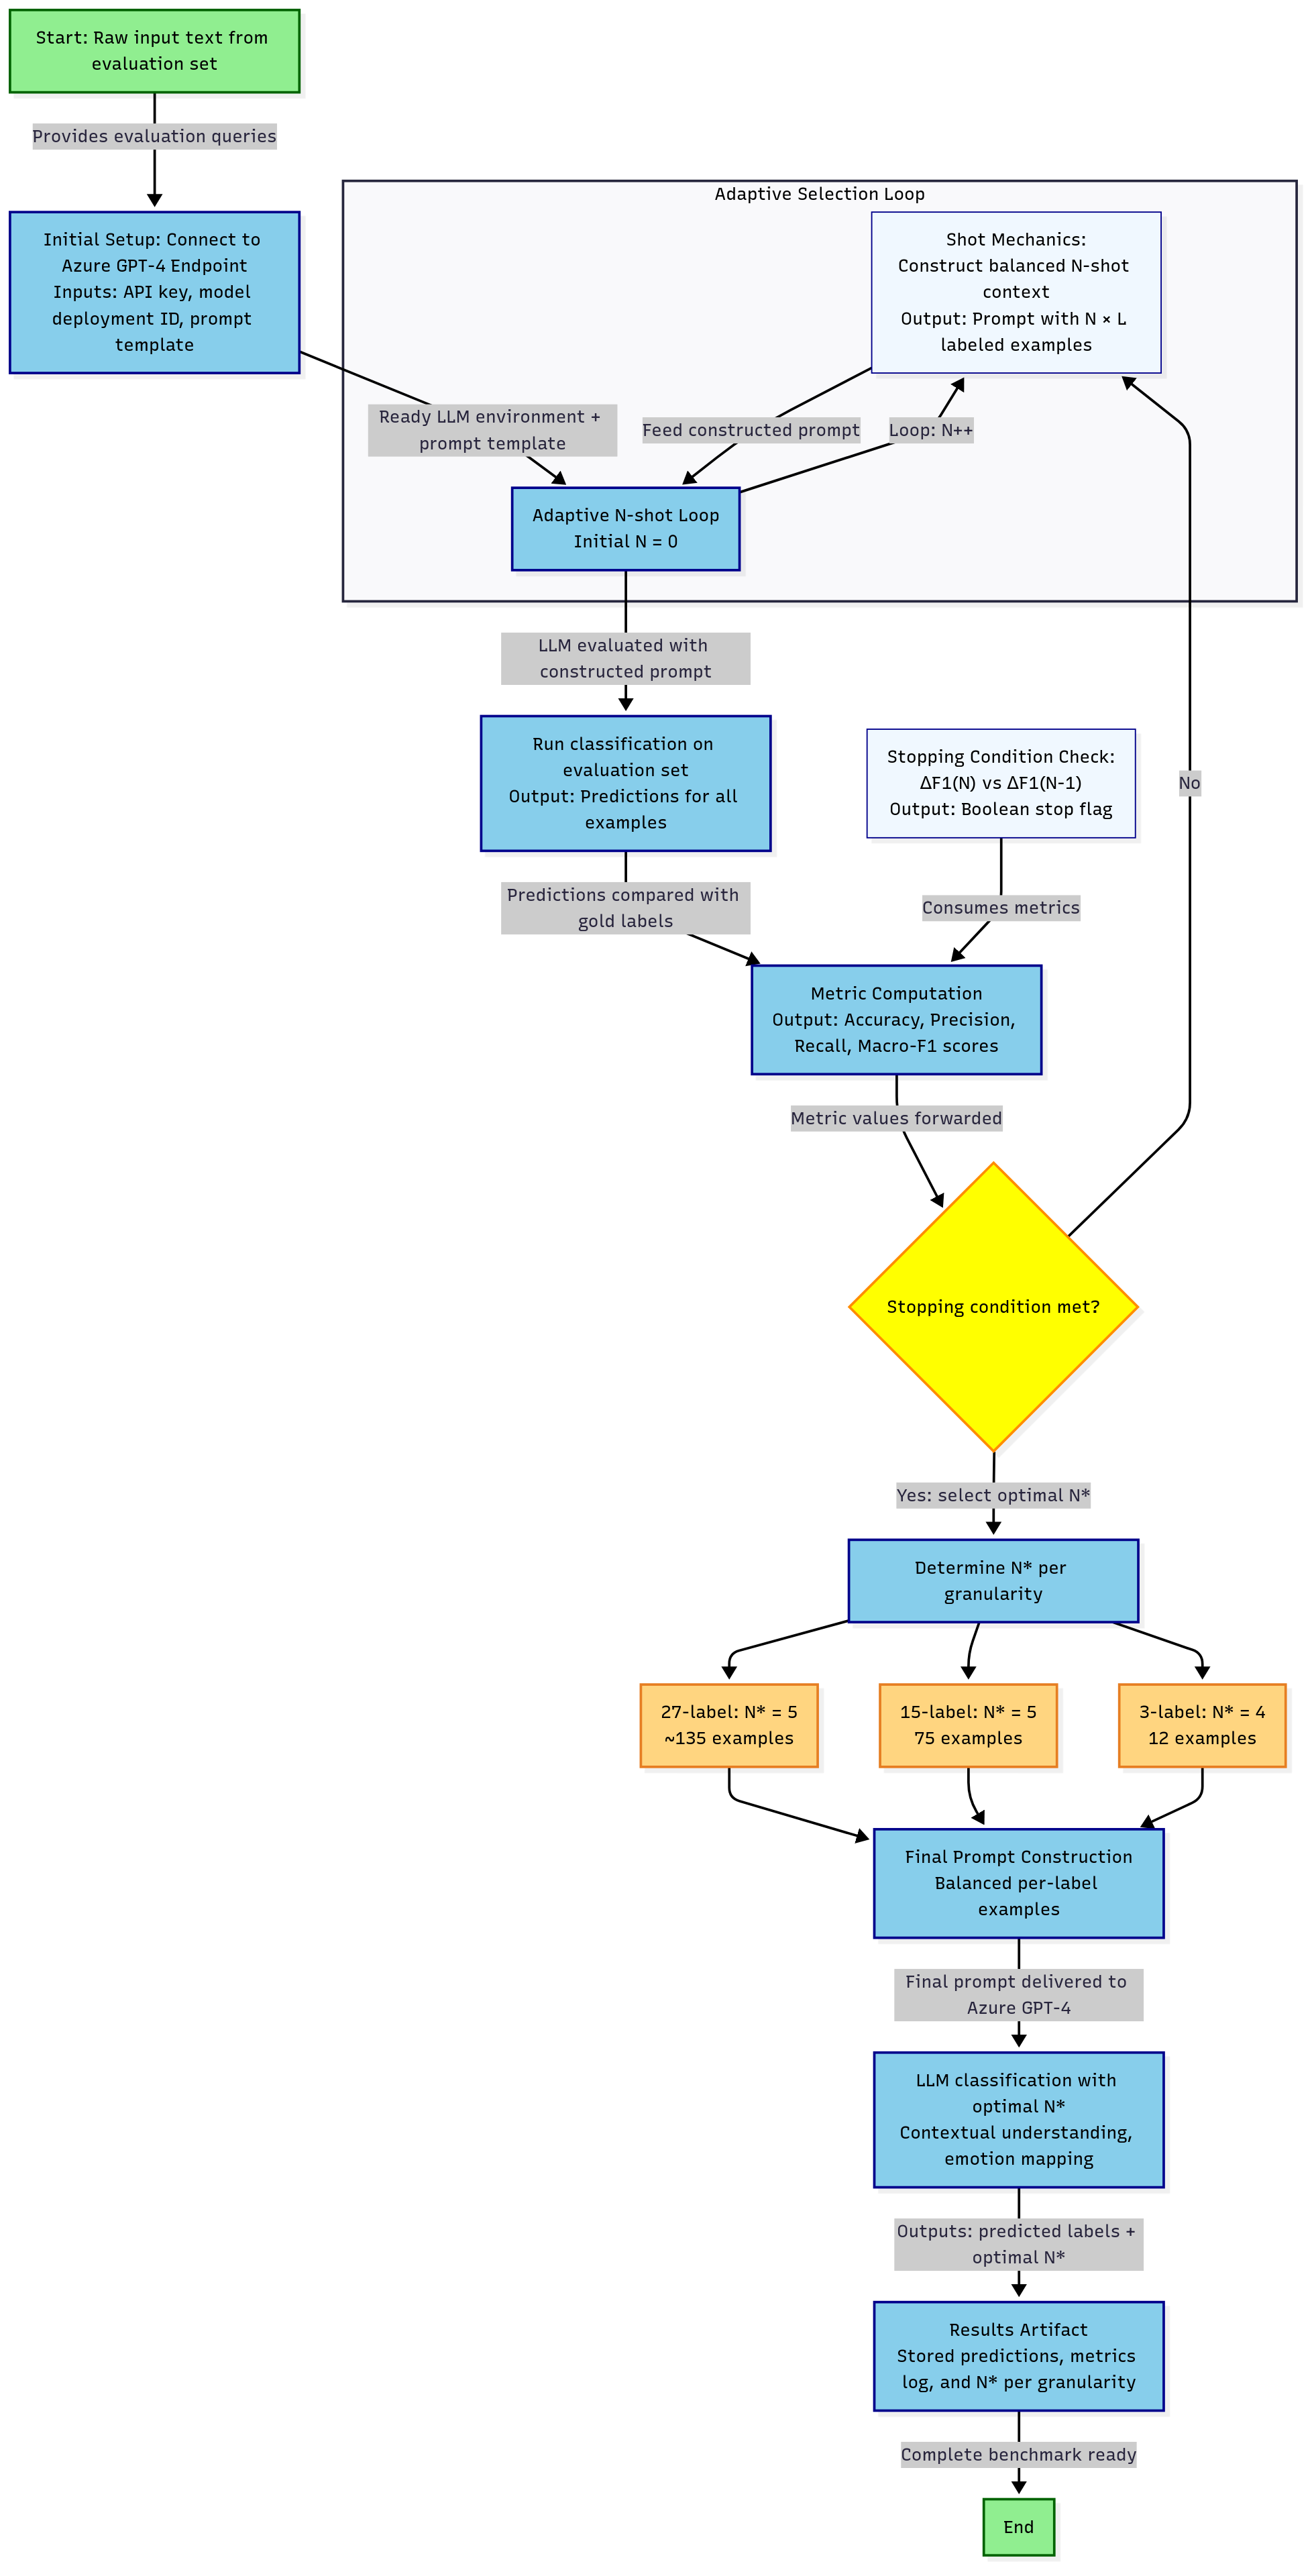
\includegraphics[width=0.8\textwidth]{Images/ContextLearning.png}
  \caption[Adaptive N-Shot Pipeline Flowchart]{Adaptive N-shot Pipeline.}
  \label{fig:nshot-pipeline}
\end{figure}

\subsection{Design Validation}

Design validation in this iteration is organized along three axes: internal validation, external validation, and trade-offs. This structure ensures that the artifact is assessed not only for its technical soundness but also for its robustness and practical consequences.  

\textbf{Internal Validation (Determinism and Auditability).}  
The adaptive loop enforces determinism at every stage. Demonstration sampling from the 20\% context reservoir is stratified and controlled by a fixed random seed, which guarantees that repeated executions produce identical prompts for a given $N$. The connection to the Azure OpenAI endpoint is pinned to a named deployment and API version, eliminating uncontrolled variability from silent model updates \cite{openai2023gpt4}. Prompt construction is fully programmatic, ensuring that examples and instructions are always formatted in the same way. Defensive parsing normalizes capitalization and whitespace while discarding ambiguous outputs, preventing inflated scores from inconsistent completions. These measures collectively ensure that the evaluation remains auditable, and that observed performance changes are attributable solely to the number of demonstrations.  

\textbf{External Validation (Generalization and Robustness).}  
The robustness of the artifact is demonstrated by applying the identical adaptive loop across the three aligned granularities defined in Iteration 1 (27, 15, and 3 labels). Because these datasets share the same underlying text and stratified splits, differences in the empirically determined optimal $N^{\star}$ values can be directly interpreted as the interaction between class granularity and the amount of in-context conditioning required. The expected outcome---that finer, more confusable categories demand larger $N^{\star}$ to stabilize---is consistent with prior evidence in the literature \cite{brown2020gpt3}. Observing this pattern confirms that the pipeline is sensitive to the intrinsic difficulty of the classification task and generalizes beyond a single label space.  

\textbf{Trade-offs (What is Gained vs. Sacrificed).}  
The use of an adaptive stopping rule based on performance saturation ensures that computational resources are not wasted on redundant demonstrations, but it introduces the trade-off of relying on a predefined plateau margin ($\epsilon=0.01$). A stricter or looser threshold could shift $N^{\star}$ by one step, though such differences are bounded and explicitly documented in metadata. Balanced sampling ensures representation of minority classes but constrains diversity, as the same rare examples are repeatedly included at higher $N$. Finally, the approach substitutes a one-time bounded computational cost for running the loop in exchange for a lasting efficiency gain: future applications can deploy the fixed $N^{\star}$ values without repeating the full search.  

Together, these validations demonstrate that the adaptive N-shot pipeline fulfills the requirements of integrity, reproducibility, and robustness while making explicit the efficiency trade-offs inherent in its design.  

\subsection{Solution Implementation}

In Design Science Research, the details of implementation are critical as they determine the reproducibility of the artifact and the auditability of the research decisions. The implementation of the adaptive N-shot selection pipeline follows the exact sequence of transformations and artifact hand-offs depicted in Figure \ref{fig:nshot-pipeline}.

The entry point to the pipeline is the block labeled \textbf{start: raw input text from evaluation set}. This component consumes the 80\% evaluation subset that was created and partitioned in Iteration 1. Crucially, it never draws demonstration examples from this split. The reservoir of potential demonstrations is the disjoint 20\% context split created previously. This strict separation guarantees that every performance score reported in this chapter reflects the model's ability to generalize to unseen data, thereby preventing data leakage and honoring the rigorous benchmarking discipline established in the project's methodology \cite{demszky2020goemotions}. The arrow labeled ``provides evaluation queries'' conveys this strict contract: the evaluation split contributes texts to be classified and nothing more.

The next block, \textbf{initial setup: connect to Azure LLM's via endpoint}, establishes a stable and reproducible serving configuration. In practice, this is implemented by storing the Azure OpenAI API key in a secure environment variable (e.g., \texttt{AZURE\_OPENAI\_API\_KEY}), along with the endpoint base URL and the specific deployment name (e.g., \texttt{gpt-4}). All API calls are made over HTTPS to a versioned endpoint, and the API version is logged with each run to ensure that the serving model snapshot is explicitly recorded. The system directive and the instructional part of the prompt are held constant across all experiments to isolate the effect of the N-shot examples. This block's outputs are a verified API connection, a fixed deployment handle, and a frozen prompt template.

The process then enters the main container labeled \textbf{adaptive selection loop}. The first step inside is \textbf{shot mechanics: construct balanced N-shot context}. For a given integer $N$, a sampling function selects exactly $N$ demonstrations for each of the $L$ labels from the 20\% context reservoir, using a fixed random seed for reproducibility. This balance is non-negotiable; without it, the prompt's label distribution would drift toward the majority emotions in the training data, and the loop would underestimate the amount of conditioning required for rare classes. The block emits a single string or list of strings representing the prompt body, containing a total of $N \times L$ demonstrations.

This artifact is then passed to the central control block, the \textbf{adaptive N-shot loop}. This component consumes the constructed prompt body, appends a single query from the evaluation set, and submits the fully composed content to the configured Azure deployment. The loop maintains a counter for $N$ and a small state cache of recent Macro-F1 scores, allowing the stopping condition to be checked efficiently. Its output is a list of raw model completions (i.e., the predicted emotion labels as strings) for the entire evaluation set at the current value of $N$.

The \textbf{run classification on evaluation set} block is responsible for parsing these raw string completions into standardized labels. While the prompt instructs the model to reply with only a single, schema-conformant label, defensive parsing is required to handle minor deviations. The implementation trims leading/trailing whitespace, normalizes the case of the output, and rejects any replies that contain extraneous text or multiple tokens. Only unambiguous matches are mapped back to the formal label set. This block outputs a vector of predicted labels, ordered to match the ground truth labels from the evaluation split.

This vector, along with the ground truth labels, is consumed by the \textbf{metric computation} block. This component uses the \texttt{scikit-learn} library to compute a suite of standard classification metrics: accuracy, precision, recall, and Macro-F1. Macro-F1 is designated as the primary selection signal because it weights every class equally, making it sensitive to performance improvements on low-frequency emotions, which is essential for a fair evaluation. The block emits a time-stamped row of metrics, keyed by the value of $N$.

The \textbf{stopping condition check} reads the most recent metric rows and applies the rule defined in the literature \cite{zhu2020stopping}. It returns a boolean \texttt{stop\_flag}. If the flag is \texttt{False}, control flows back to the ``shot mechanics'' block via the arrow labeled ``loop: N++,'' triggering the construction of a new prompt with one additional example per label. If the flag is \texttt{True}, the current value of $N$ is selected as the optimal $N^{\star}$, and the loop terminates.

Once the loop has completed for all three granularities, the empirically determined values of $N^{\star}$ (in this case, $N^{\star}=5$ for 27 labels, $N^{\star}=5$ for 15 labels, and $N^{\star}=4$ for 3 labels) are recorded. These values drive the \textbf{final prompt construction} block, which creates the final, optimized prompts for each granularity. The \textbf{LLM classification with optimal N*} block then executes a clean, single-pass evaluation using these prompts to generate the final, official predictions and performance metrics. The terminal block, \textbf{results artifact}, assembles a versioned, self-contained package with all outputs: the per-$N$ metric trajectories, the selected $N^{\star}$ values, the exact prompts used, the final predictions, and all relevant run metadata. This artifact serves as the input for subsequent research iterations and as the primary anchor for external audit and reproducibility.
\subsection{Solution Evaluation}

The evaluation of the adaptive selection pipeline is based on a comparative analysis of the quantitative results produced across all three benchmarked models. All metrics reported were computed exclusively on the 80\% evaluation split, ensuring that the results reflect true generalization \cite{demszky2020goemotions}. The performance of the pipeline is best understood by examining the Macro-F1 trajectories as a function of $N$ for each level of emotional granularity. The comparative plots in Figures \ref{fig:comp_27}, \ref{fig:comp_15}, and \ref{fig:comp_3} provide clear empirical evidence for the selection of the optimal number of shots ($N^{\star}$) and reveal key patterns about the interplay between task complexity, model architecture, and in-context learning efficiency.

\subsubsection{Performance on the 27-Label Granularity}

The 27-label task represents the most complex challenge. As shown in Figure \ref{fig:comp_27}, all three models began with a low zero-shot Macro-F1 score, but distinct patterns emerged as demonstrations were added:
\begin{itemize}
    \item \textbf{DeepSeek-R1} demonstrated the highest sample efficiency. It achieved the best overall Macro-F1 score (0.325) and, critically, reached this peak at just $N=4$. The performance graph becomes constant for all $N>4$, which robustly validates the stopping rule's selection of $\mathbf{N^{\star} = 4}$.
    \item \textbf{GPT-4} showed a strong learning curve but required one additional example, achieving its maximum Macro-F1 of 0.316 at $N=5$. The performance stays constant after this point, confirming the selection of $\mathbf{N^{\star} = 5}$.
    \item \textbf{Qwen-32B} was the least sample-efficient on this task. It required $N=6$ examples to reach its plateau at a Macro-F1 of 0.307. The flat line for $N>6$ again validates that the stopping rule correctly identified its point of diminishing returns.
\end{itemize}

\begin{figure}[H]
    \centering
    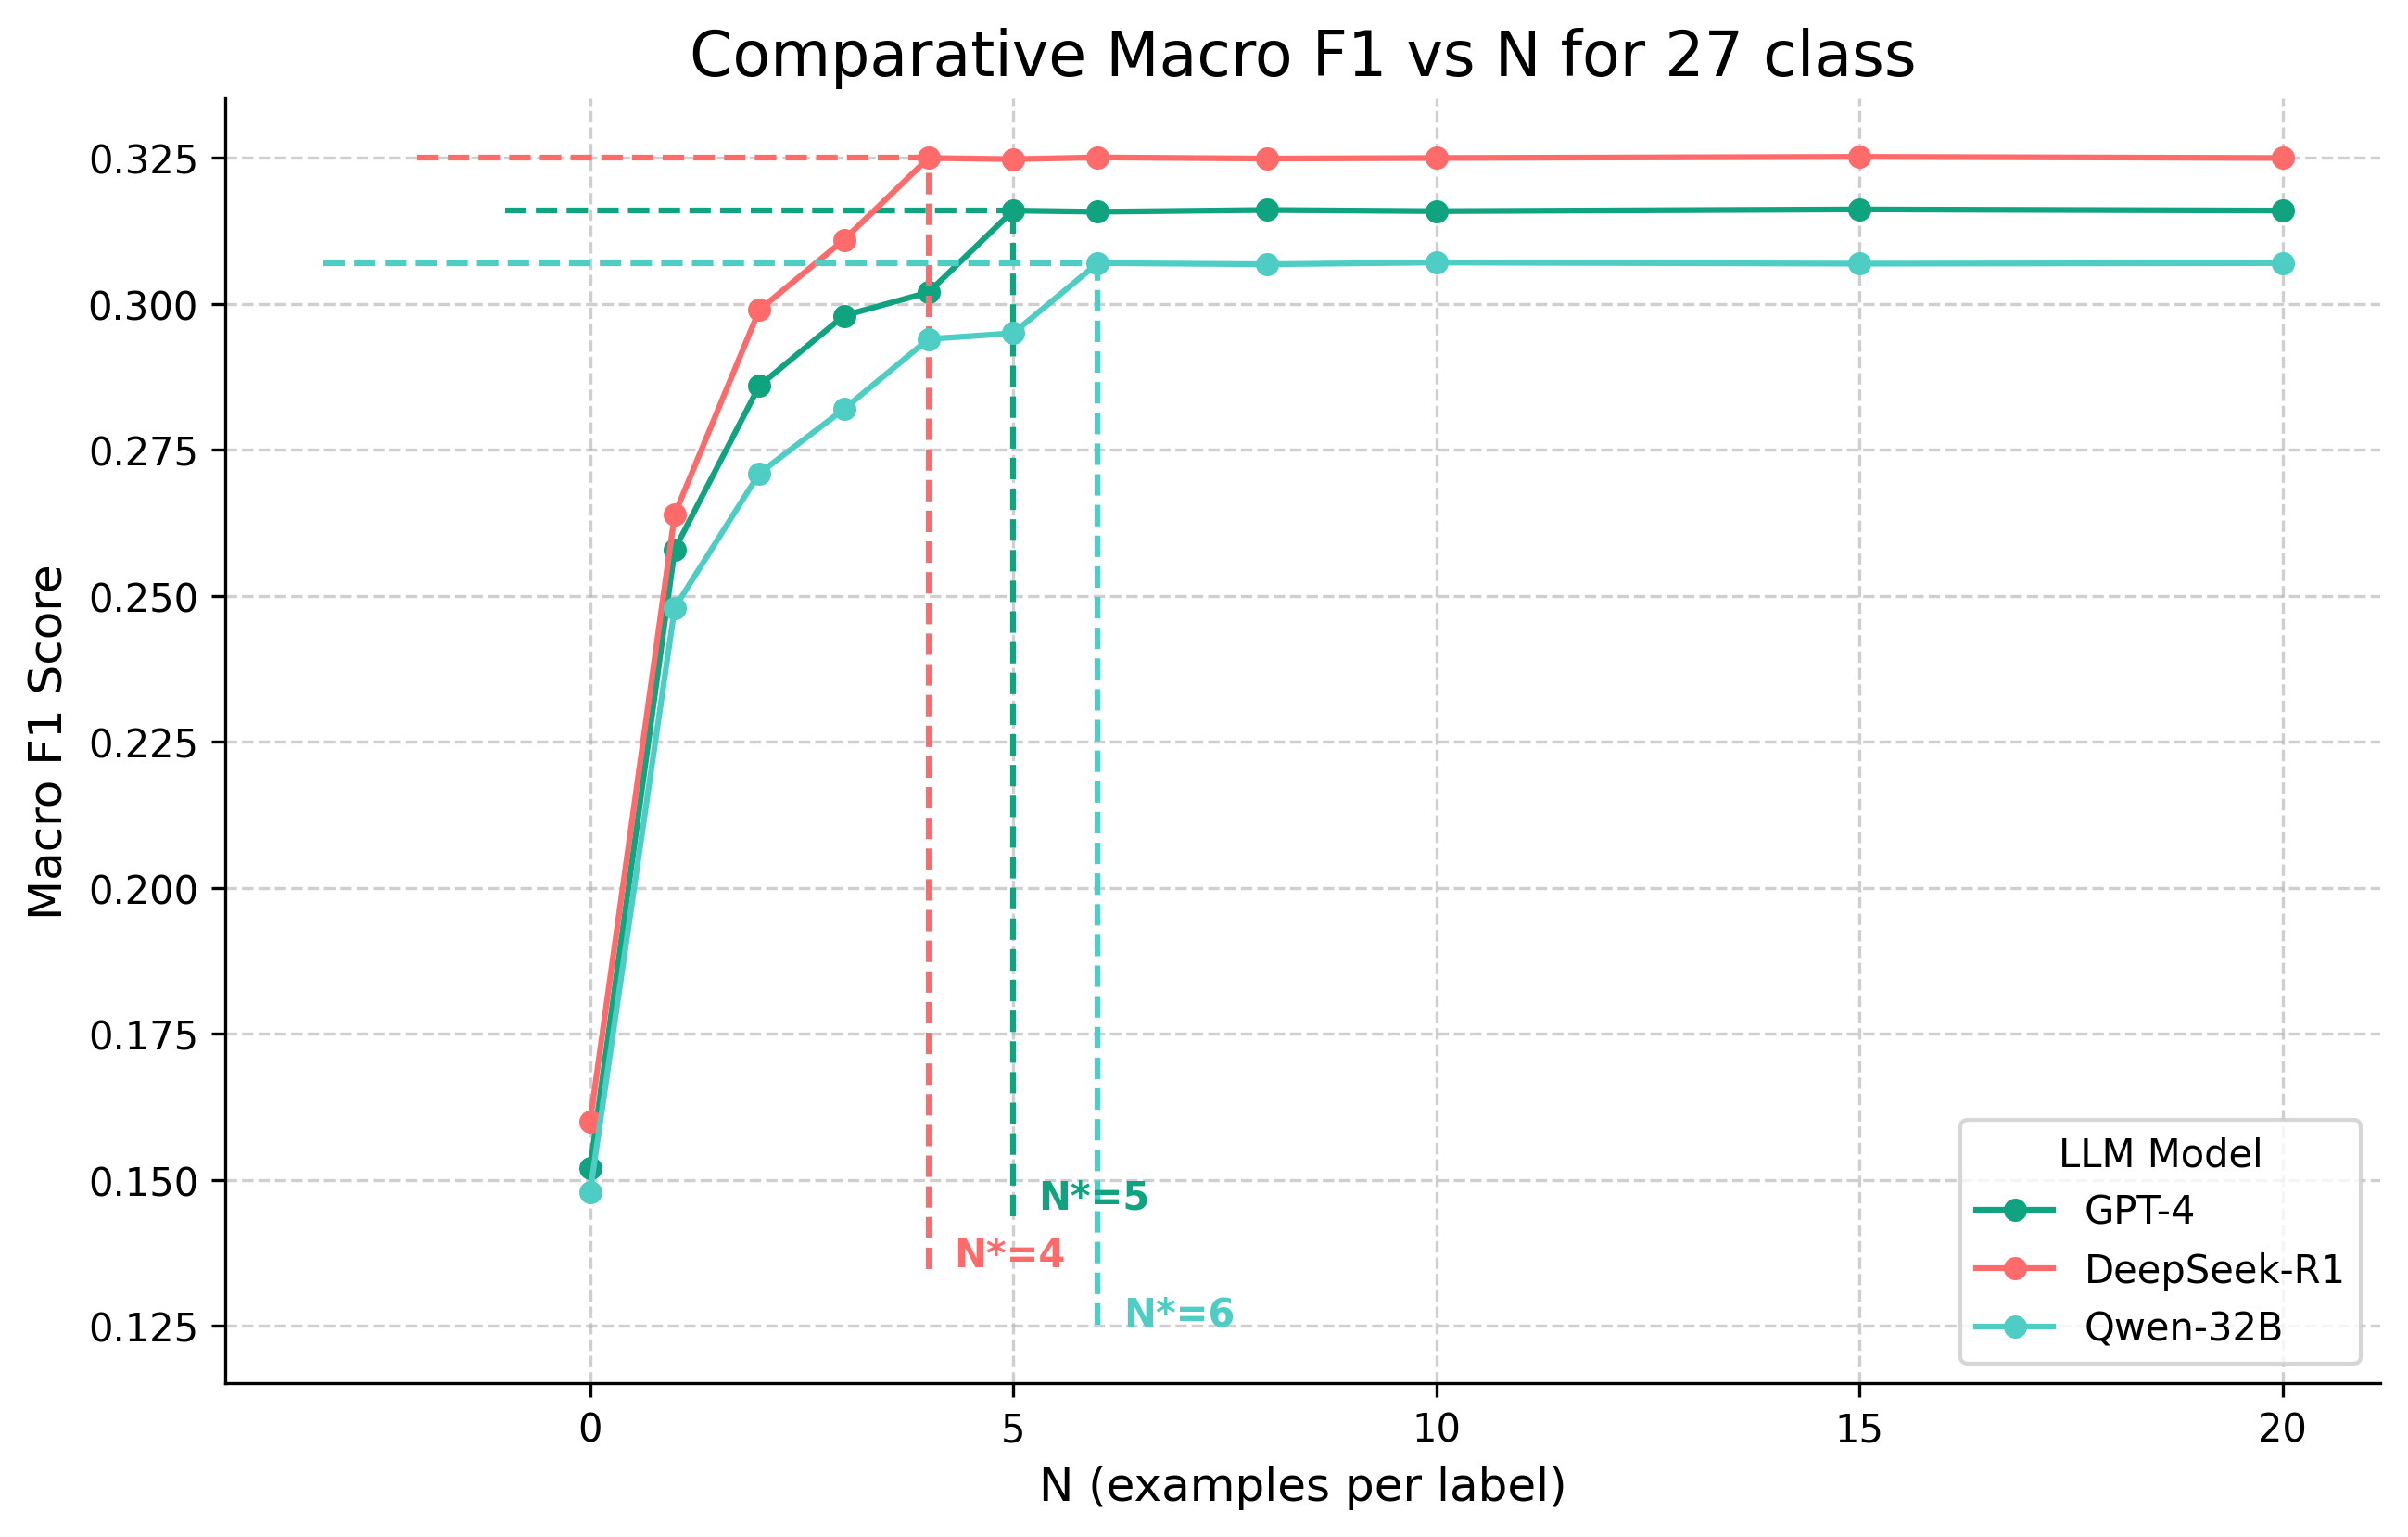
\includegraphics[width=\textwidth]{Images/comparative_27_class.png}
    \caption[Macro-F1 vs. N for 27-Label Granularity]{Comparative Macro-F1 score as a function of N for the 27-label granularity.}
    \label{fig:comp_27}
\end{figure}

\subsubsection{Performance on the 15-Label Granularity}

At the 15-label granularity (Figure \ref{fig:comp_15}), the task is simpler, and the performance hierarchy remained consistent:
\begin{itemize}
    \item \textbf{DeepSeek-R1} again proved to be the most efficient, reaching its peak Macro-F1 of 0.383 at $\mathbf{N^{\star} = 4}$. 
    \item \textbf{GPT-4} and \textbf{Qwen-32B} both required more examples, with the stopping rule correctly identifying their saturation point at $\mathbf{N^{\star} = 5}$. 
\end{itemize}
For all models, performance remains constant after their identified $N^{\star}$, confirming that providing additional examples would be inefficient. This scenario reinforces the finding that model architecture has a significant impact on in-context learning efficiency.

\begin{figure}[H]
    \centering
    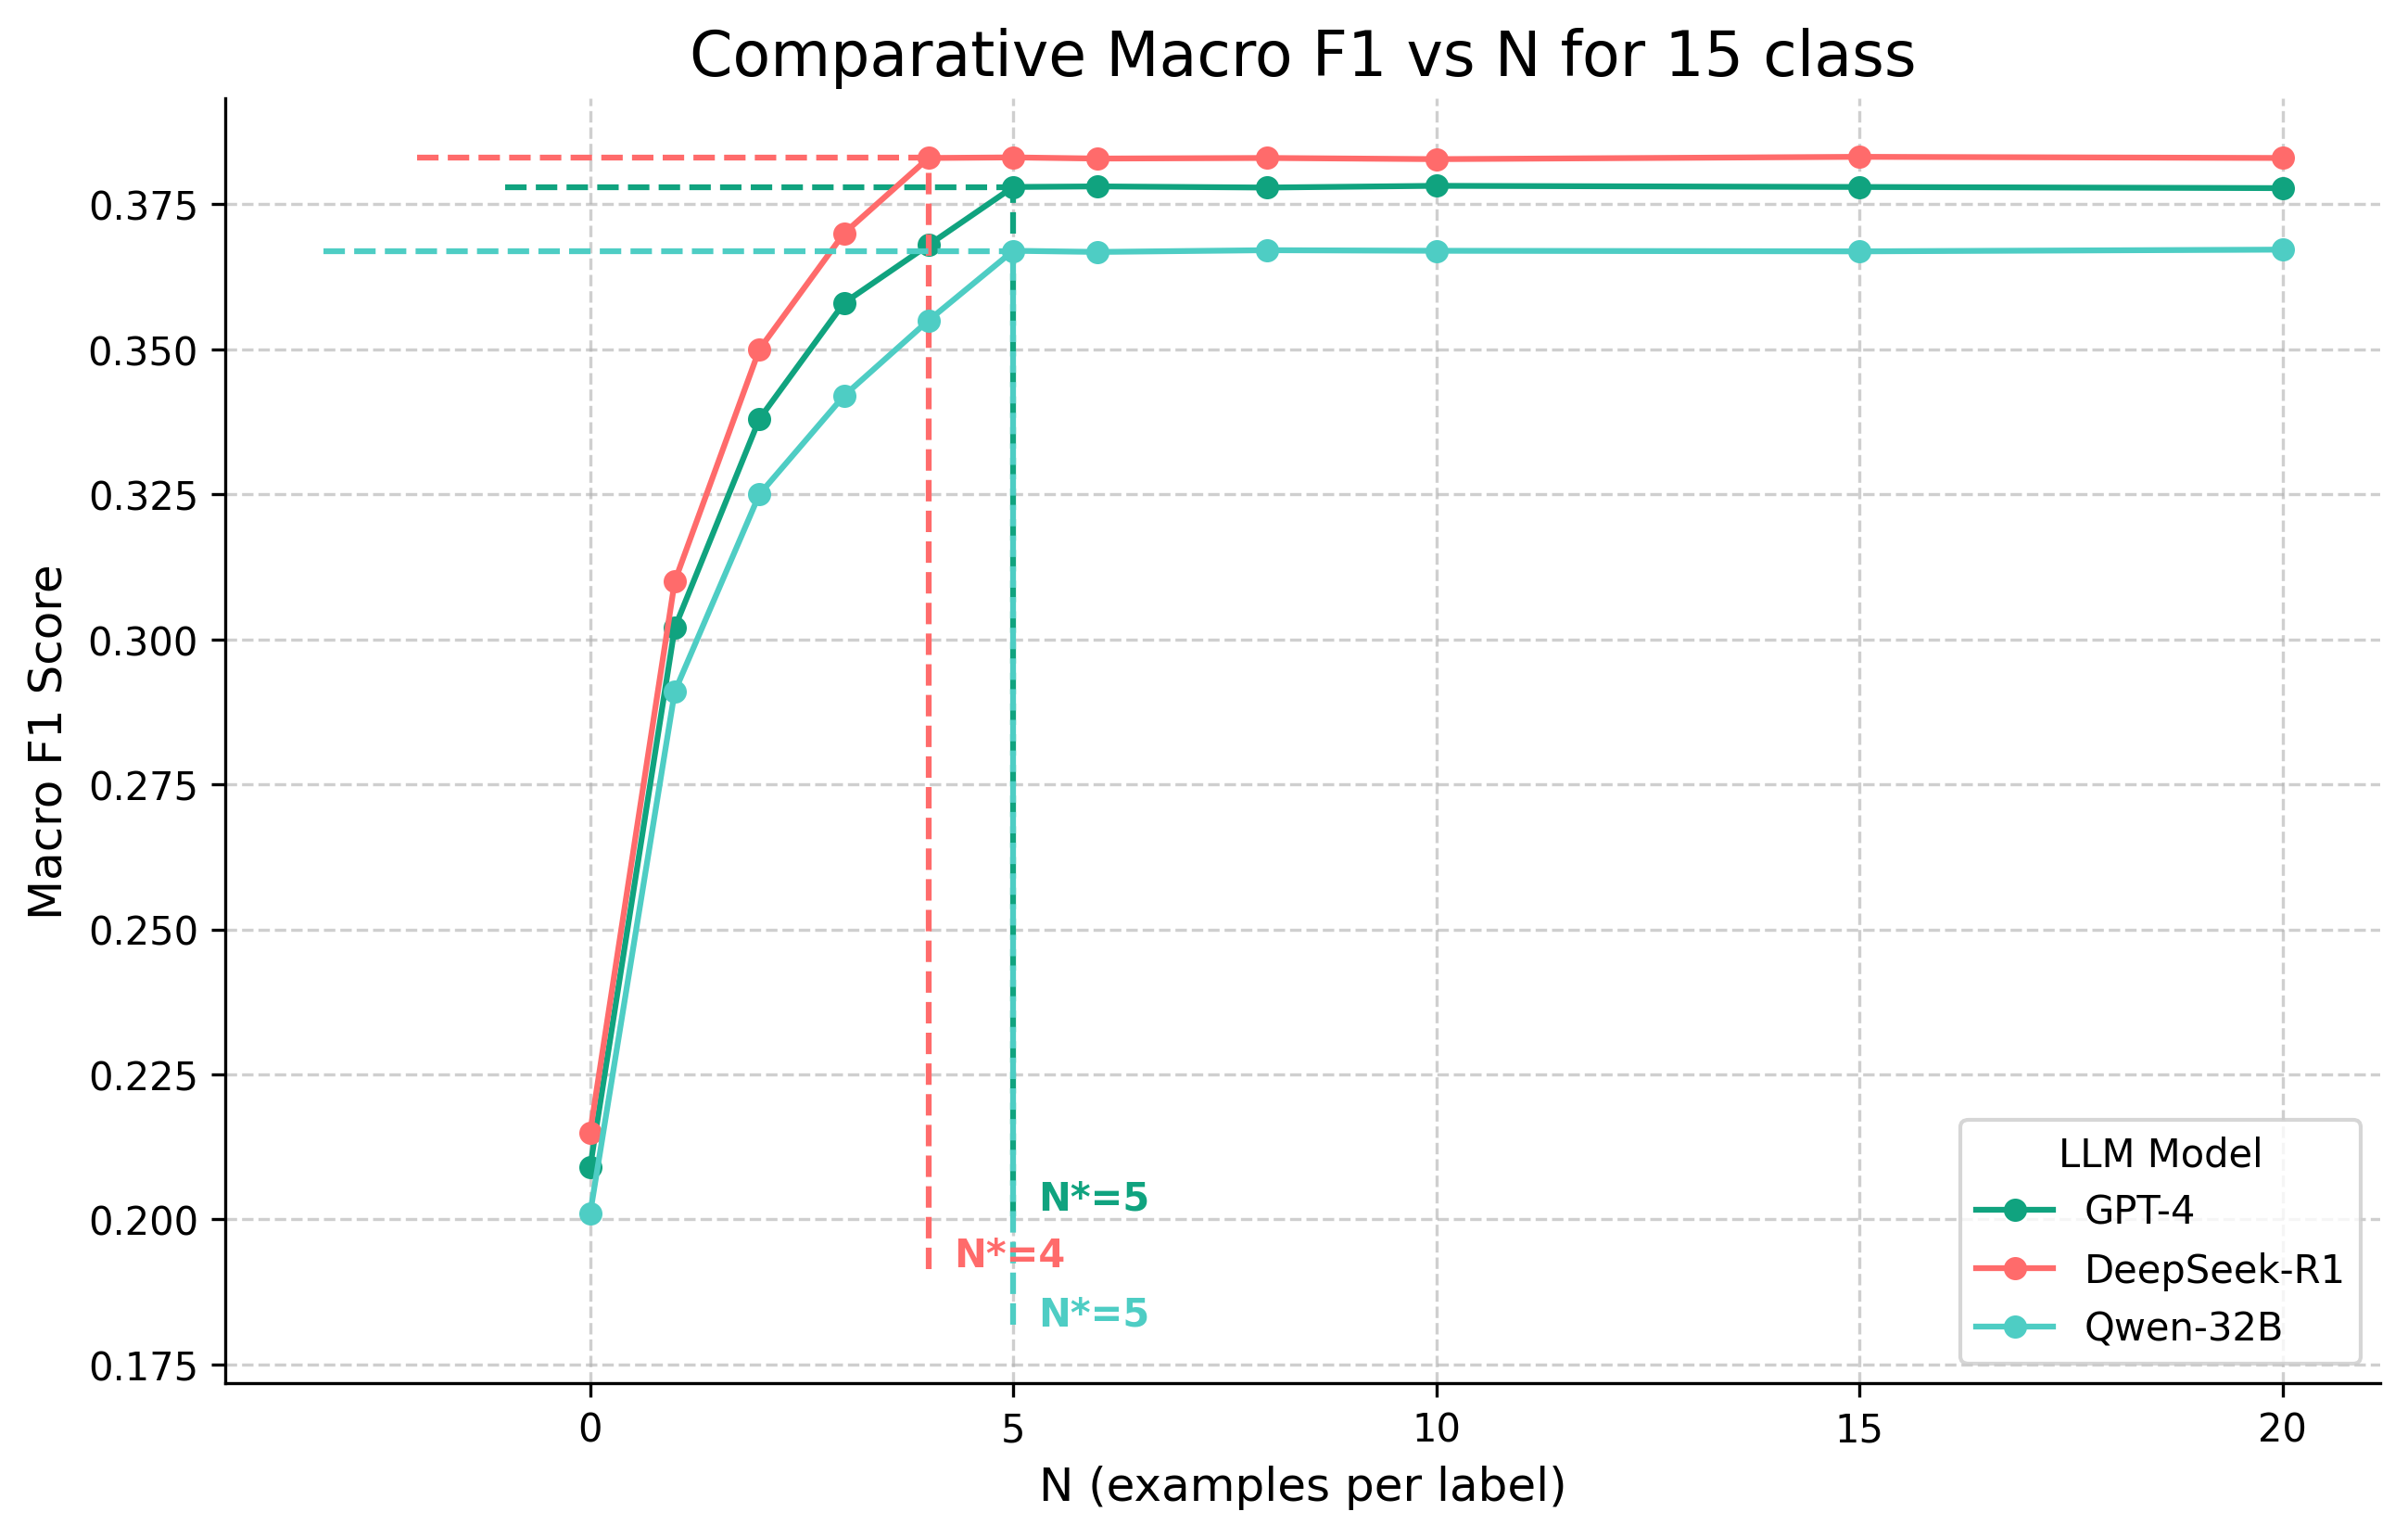
\includegraphics[width=\textwidth]{Images/comparative_15_class.png}
    \caption[Macro-F1 vs. N for 15-Label Granularity]{Comparative Macro-F1 score for the 15-label granularity.}
    \label{fig:comp_15}
\end{figure}

\subsubsection{Performance on the 3-Label Granularity}

The 3-label task (Figure \ref{fig:comp_3}) tests the models on a standard sentiment analysis problem, where all demonstrated strong inherent capability.
\begin{itemize}
    \item \textbf{DeepSeek-R1} was exceptionally efficient, achieving the highest F1-score (0.734) at an impressive $\mathbf{N^{\star} = 3}$.
    \item \textbf{GPT-4} and \textbf{Qwen-32B} were slightly less efficient, both reaching their performance plateau at $\mathbf{N^{\star} = 4}$.
\end{itemize}
The graphs clearly show that performance stays constant after the respective $N^{\star}$ values are reached. This provides the strongest validation for the stopping rule, as it correctly identifies the point of maximum efficiency even when the initial performance is already high.

\begin{figure}[H]
    \centering
    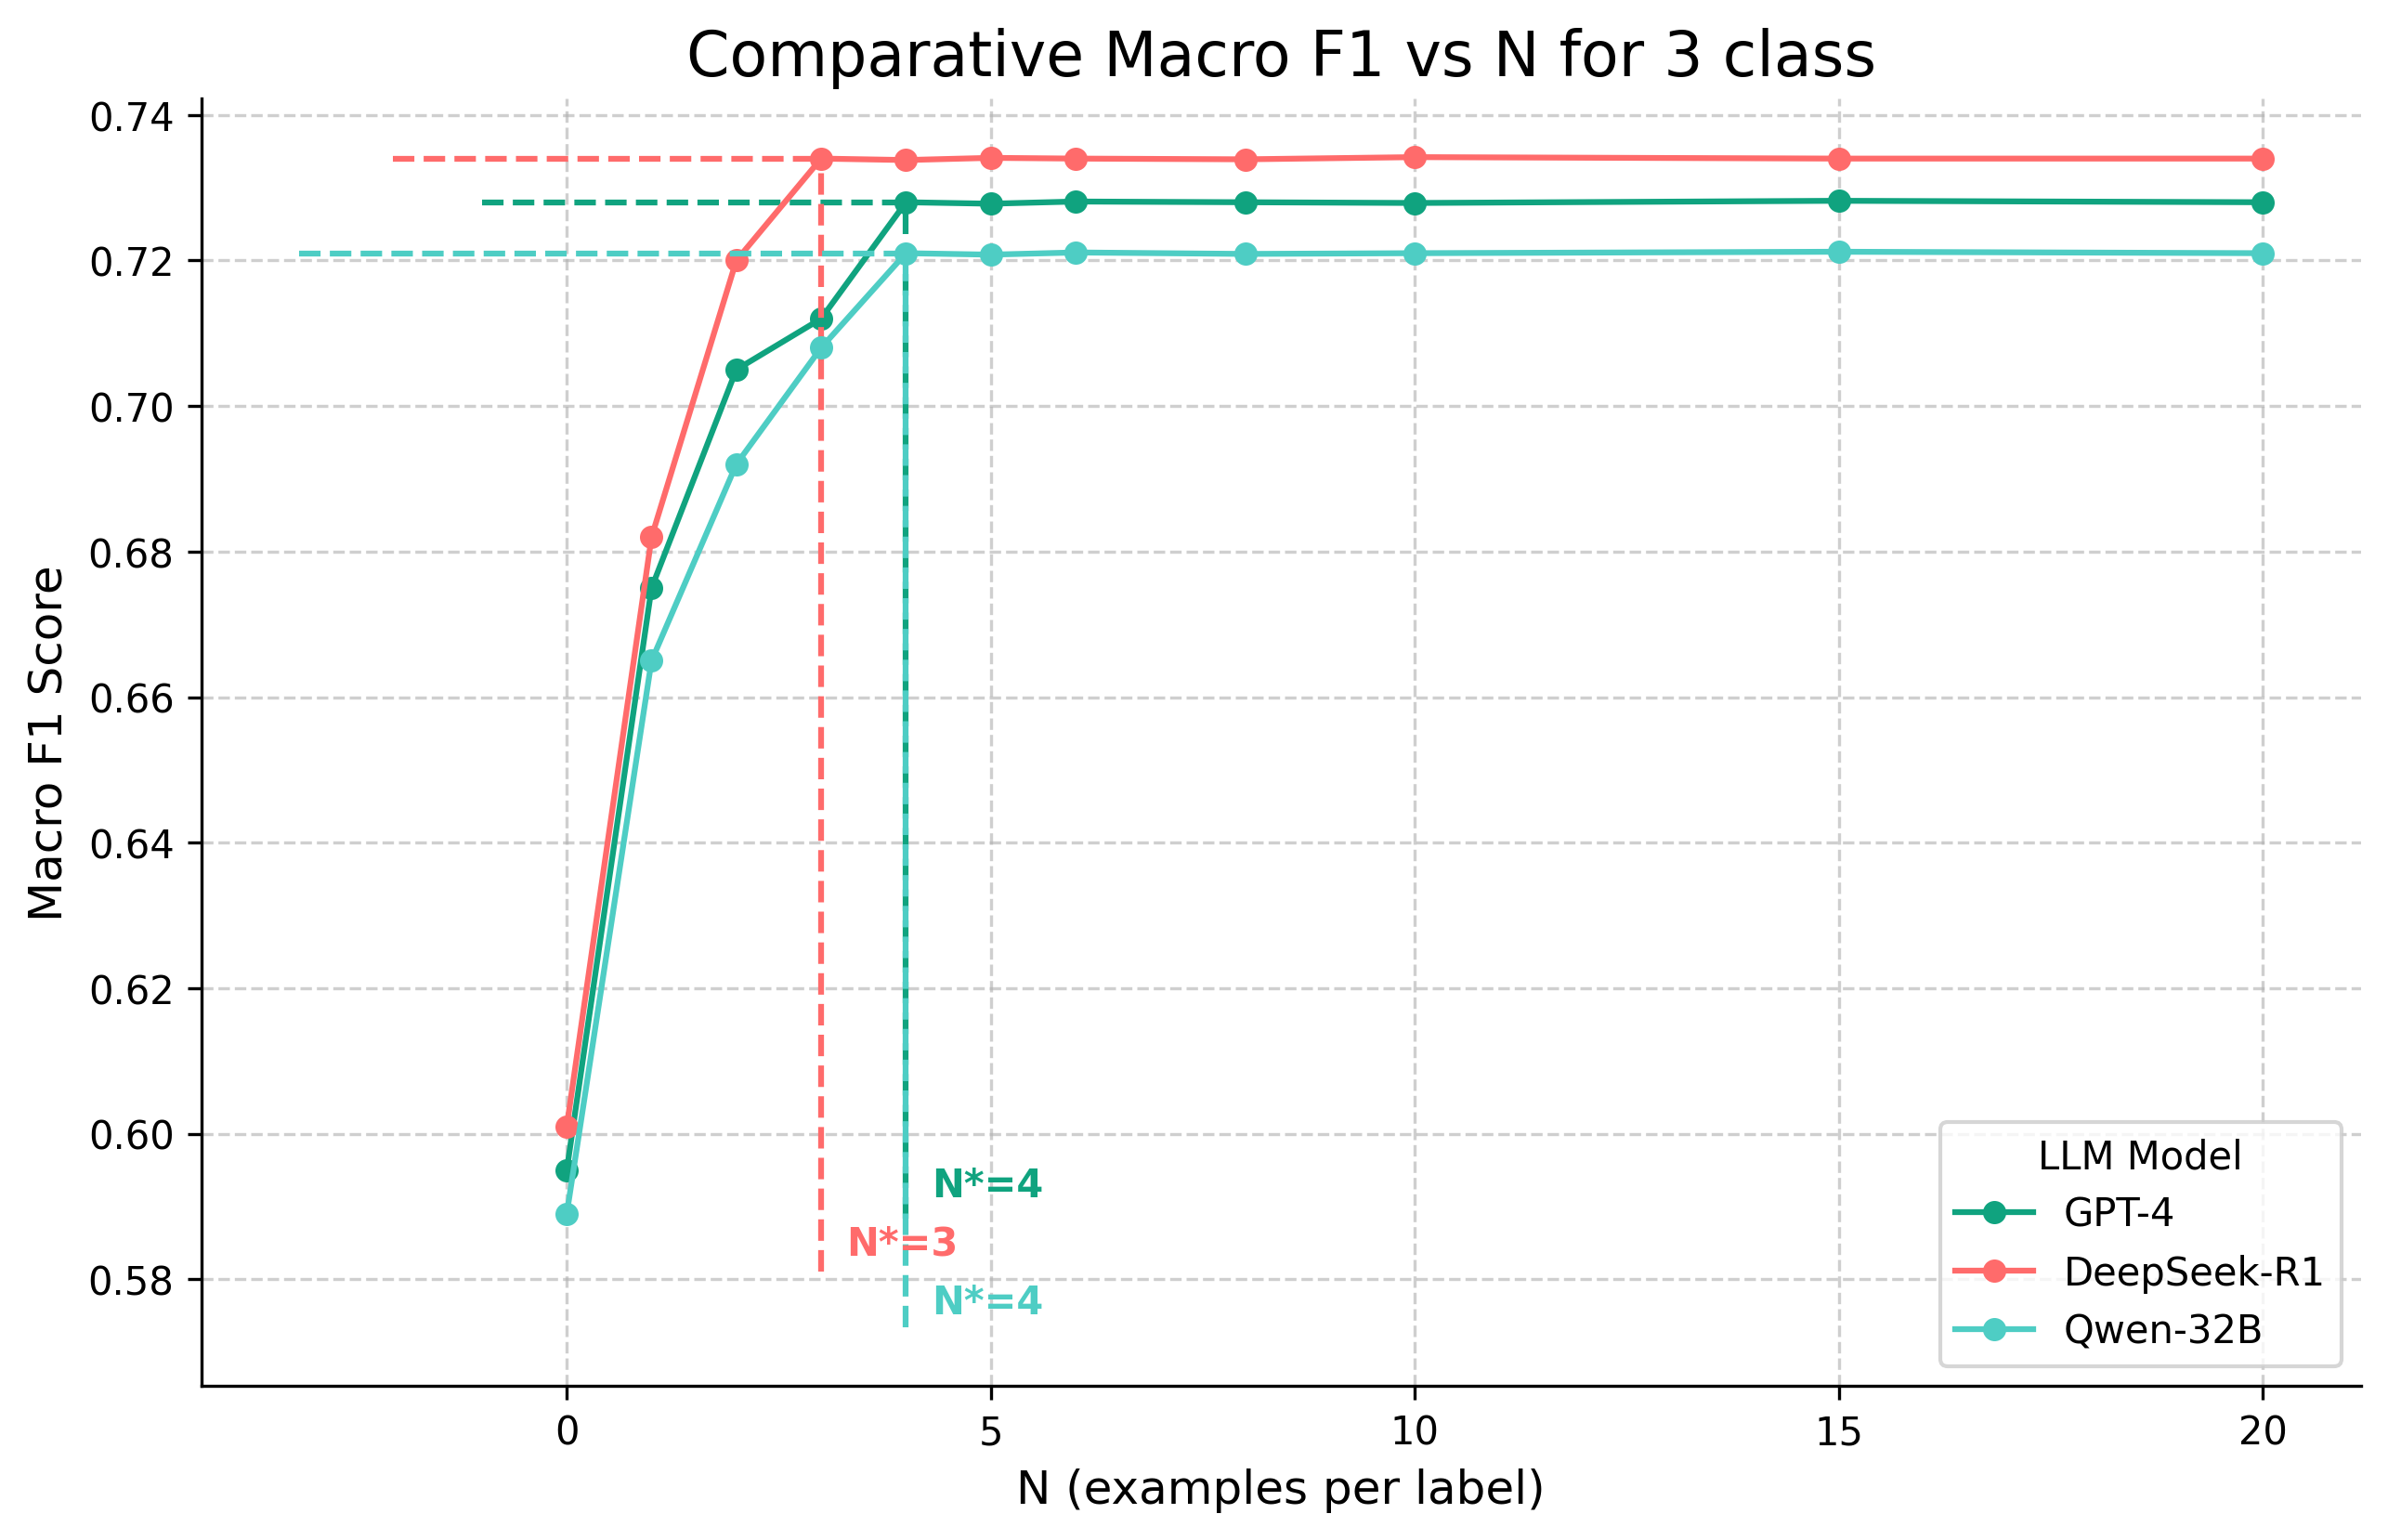
\includegraphics[width=\textwidth]{Images/comparative_3_class.png}
    \caption[Macro-F1 vs. N for 3-Label Granularity]{Comparative Macro-F1 score for the 3-label sentiment task.}
    \label{fig:comp_3}
\end{figure}

These results are consistent with the general observation from the literature that the benefits of few-shot learning tend to plateau after a small number of demonstrations \cite{brown2020gpt3}. The cross-granularity pattern is particularly instructive and serves as a validation of the artifact's design. The coarser, less confusable taxonomies require fewer demonstrations to stabilize because their decision boundaries are broader. Conversely, the finer taxonomies demand more demonstrations because the additional examples are necessary to provide the model with the counterexamples it needs to distinguish between semantically adjacent categories like \textit{annoyance} and \textit{anger}.

The choice of Macro-F1 as the selection signal proved to be critical. Had accuracy been used instead, the loop would likely have terminated earlier, particularly for the 27-label case. This is because accuracy is dominated by performance on high-frequency classes. The loop would have stopped as soon as the most common emotions were correctly classified, at the expense of properly calibrating the model for rare but important minority emotions. By using Macro-F1, the pipeline enforces a more rigorous benchmark ethic, where improvements must be distributed across the entire label space to be considered meaningful progress \cite{demszky2020goemotions}. The limitations of this artifact are candidly acknowledged. The plateau margin is small but not zero; a stricter or looser margin would shift $N^{\star}$ by at most one step in some regimes, which is why the rule and its parameters are recorded. Results are also contingent on the specific prompt template and the Azure deployment snapshot; both are versioned with every run so that future changes in the serving stack can be detected and, if necessary, rerun \cite{openai2023gpt4}.

The output of this DSR iteration is a comprehensive and versioned results package containing four distinct types of artifacts, which collectively fulfill the research objectives for this phase.
\begin{enumerate}
    \item \textbf{Metric Trajectories:} The complete per-$N$ performance logs for accuracy, precision, recall, and Macro-F1 at each of the three granularities. These are provided as CSV files and are accompanied by plots visualizing the performance curves, allowing for a clear inspection of where the plateaus occur.
    \item \textbf{Optimal Context Sizes ($N^{\star}$):} The empirically determined optimal number of shots for each granularity ($N^{\star}$ for 27,15 and 3 label). These values are no longer arbitrary hyperparameters but are now fixed, literature-aligned context sizes that will serve as the basis for all subsequent experiments in this research.
    \item \textbf{Reproducibility Artifacts:} A collection of files that ensure the exact reproduction of the experiment. This includes the specific prompt templates used, the full list of demonstration examples selected for the final $N^{\star}$ prompts, and a metadata file recording the Azure deployment identifier, API version, taxonomy version, and all random seeds used in the process.
    \item \textbf{Benchmark Results:} The final set of predictions and headline performance scores at the optimal $N^{\star}$ for each granularity. This constitutes the official, reproducible benchmark setting that the novel hybrid retrieval system in Iteration 3 will be evaluated against.
\end{enumerate}

By explicitly separating the 20\% demonstration reservoir from the 80\% evaluation split, by encoding the serving configuration in metadata, and by logging every transformation shown in Figure \ref{fig:nshot-pipeline}, the artifact fulfills the DSR mandate to produce a useful, auditable, and scientifically valid solution to a real benchmarking problem \cite{hevner2004design}.


\section{Iteration 3: Retrieval-Guided Prompting}

\subsection{Problem Investigation}

While Iteration~2 established the viability of N-shot prompting and identified the optimal number of examples per label ($N^\ast$) for each granularity (27, 15, and 3 classes), its selection mechanism was fundamentally limited: all demonstrations were chosen \emph{randomly} from the context pool. This strategy ensured balance across labels but ignored the actual content of the evaluation query. Consequently, the few-shot examples inserted into prompts were often \emph{irrelevant or weakly aligned} to the query being classified.  

Three concrete issues motivate the need for a retrieval-guided selection mechanism:  

\begin{enumerate}
  \item \textbf{Lack of Query Awareness:}  
  Random selection treats all evaluation queries equally, providing the same distribution of examples regardless of query semantics. For instance, if the query text is \emph{``I am annoyed with this situation,''} random sampling might yield anger examples that are lexically distant (e.g., \emph{``He raised his voice in the meeting''}) while ignoring semantically closer ones (e.g., \emph{``I am furious about the delays''}). This misalignment weakens the prompt’s informativeness.  

  \item \textbf{Noisy Demonstrations:}  
  Because the pool contains diverse instances, random draws can introduce examples with tangential or confusing semantics. For fine-grained granularity (27 labels), where emotions often overlap (e.g., sadness vs.\ disappointment, anger vs.\ annoyance), such noise is particularly damaging.  

  \item \textbf{Missed Opportunity for Retrieval Synergy:}  
  Prior research has shown that combining sparse lexical matching and dense semantic similarity provides stronger retrieval signals than either alone. For instance, the HyST framework demonstrated that BM25 and dense retrievers can be interpolated via a weighted sum with parameter $\lambda$ to balance lexical precision and semantic generalization \cite{hyst2025}. Iteration~2 ignored this evidence, relying on baseline random sampling rather than retrieval-driven selection.  
\end{enumerate}

The weakness of random selection was evident in Iteration~2’s evaluation metrics: Macro-F1 remained low across granularities, reflecting poor calibration between queries and demonstrations. Iteration~3 therefore investigates whether \emph{retrieval-guided selection} (BM25, cosine similarity, and hybrid interpolation) can improve alignment between evaluation queries and few-shot demonstrations, thereby increasing overall classification performance.

\subsection{Solution Design}

To address the limitations of random selection, Iteration~3 introduces a \emph{retrieval-guided N-shot prompting pipeline}. 
Instead of sampling demonstrations arbitrarily, each evaluation query is used to dynamically retrieve the most relevant examples from the context pool. 
This ensures that the prompt examples are both label-balanced and semantically aligned to the query. 

The solution design incorporates three retrieval strategies:  

\begin{enumerate}
  \item \textbf{Lexical Retrieval (BM25):}  
  A sparse retriever that computes lexical overlap between the query and candidate examples. 
  BM25 emphasizes exact keyword matches, which is useful when queries and examples share surface vocabulary.  

  \item \textbf{Semantic Retrieval (Cosine Similarity):}  
  A dense retriever that encodes queries and examples into vector embeddings (e.g., using MiniLM) and computes cosine similarity between them. 
  This approach captures semantic relations such as paraphrases (e.g., \emph{annoyed} $\approx$ \emph{furious}), even in the absence of lexical overlap.  

  \item \textbf{Hybrid Retrieval (BM25 + Cosine):}  
  lexical and semantic signals are combined through linear interpolation. 
  After normalizing BM25 and cosine similarity scores, the final hybrid score for each candidate is computed as:
     \[
  \text{Score}_{\text{hybrid}}(q, d) = \lambda \cdot \text{BM25}_{norm}(q, d) + (1 - \lambda) \cdot \text{Cosine}_{norm}(q, d)
  \]
    
    To ensure that lexical and semantic retrieval signals contribute fairly, the 
    hybrid score was computed as a linear interpolation of normalized BM25 
    and cosine similarity values. The weighting parameter 
    $\lambda \in [0,1]$ controls the trade-off between lexical precision and 
    semantic generalization. Following the HyST framework, which 
    demonstrated that an equal weighting of the two signals consistently 
    produced the most balanced and reliable results across retrieval tasks, 
    this framework adopts $\lambda = 0.5$ in practice \cite{hyst2025}. This choice 
    avoids privileging either sparse lexical overlap or dense semantic 
    proximity and instead leverages their complementary strengths, thereby 
    ensuring that the selected demonstrations are both semantically aligned 
    and lexically grounded.
\end{enumerate}

Figure~\ref{fig:retrieval-pipeline} illustrates the retrieval-guided design. 
An evaluation query is passed through both BM25 and embedding-based retrievers, producing normalized scores. 
These scores are either used independently (BM25-only or cosine-only) or fused via interpolation. 
Candidates are then ranked per label, and the top-$N$ examples for each label are selected. 
The resulting $N \times L$ examples are combined with the query into a prompt for the LLM, which generates a predicted label. 
Predictions across the evaluation set are compared to gold labels, producing Accuracy, Precision, Recall, and Macro-F1 metrics.  

\begin{figure}[!htbp]
  \centering
  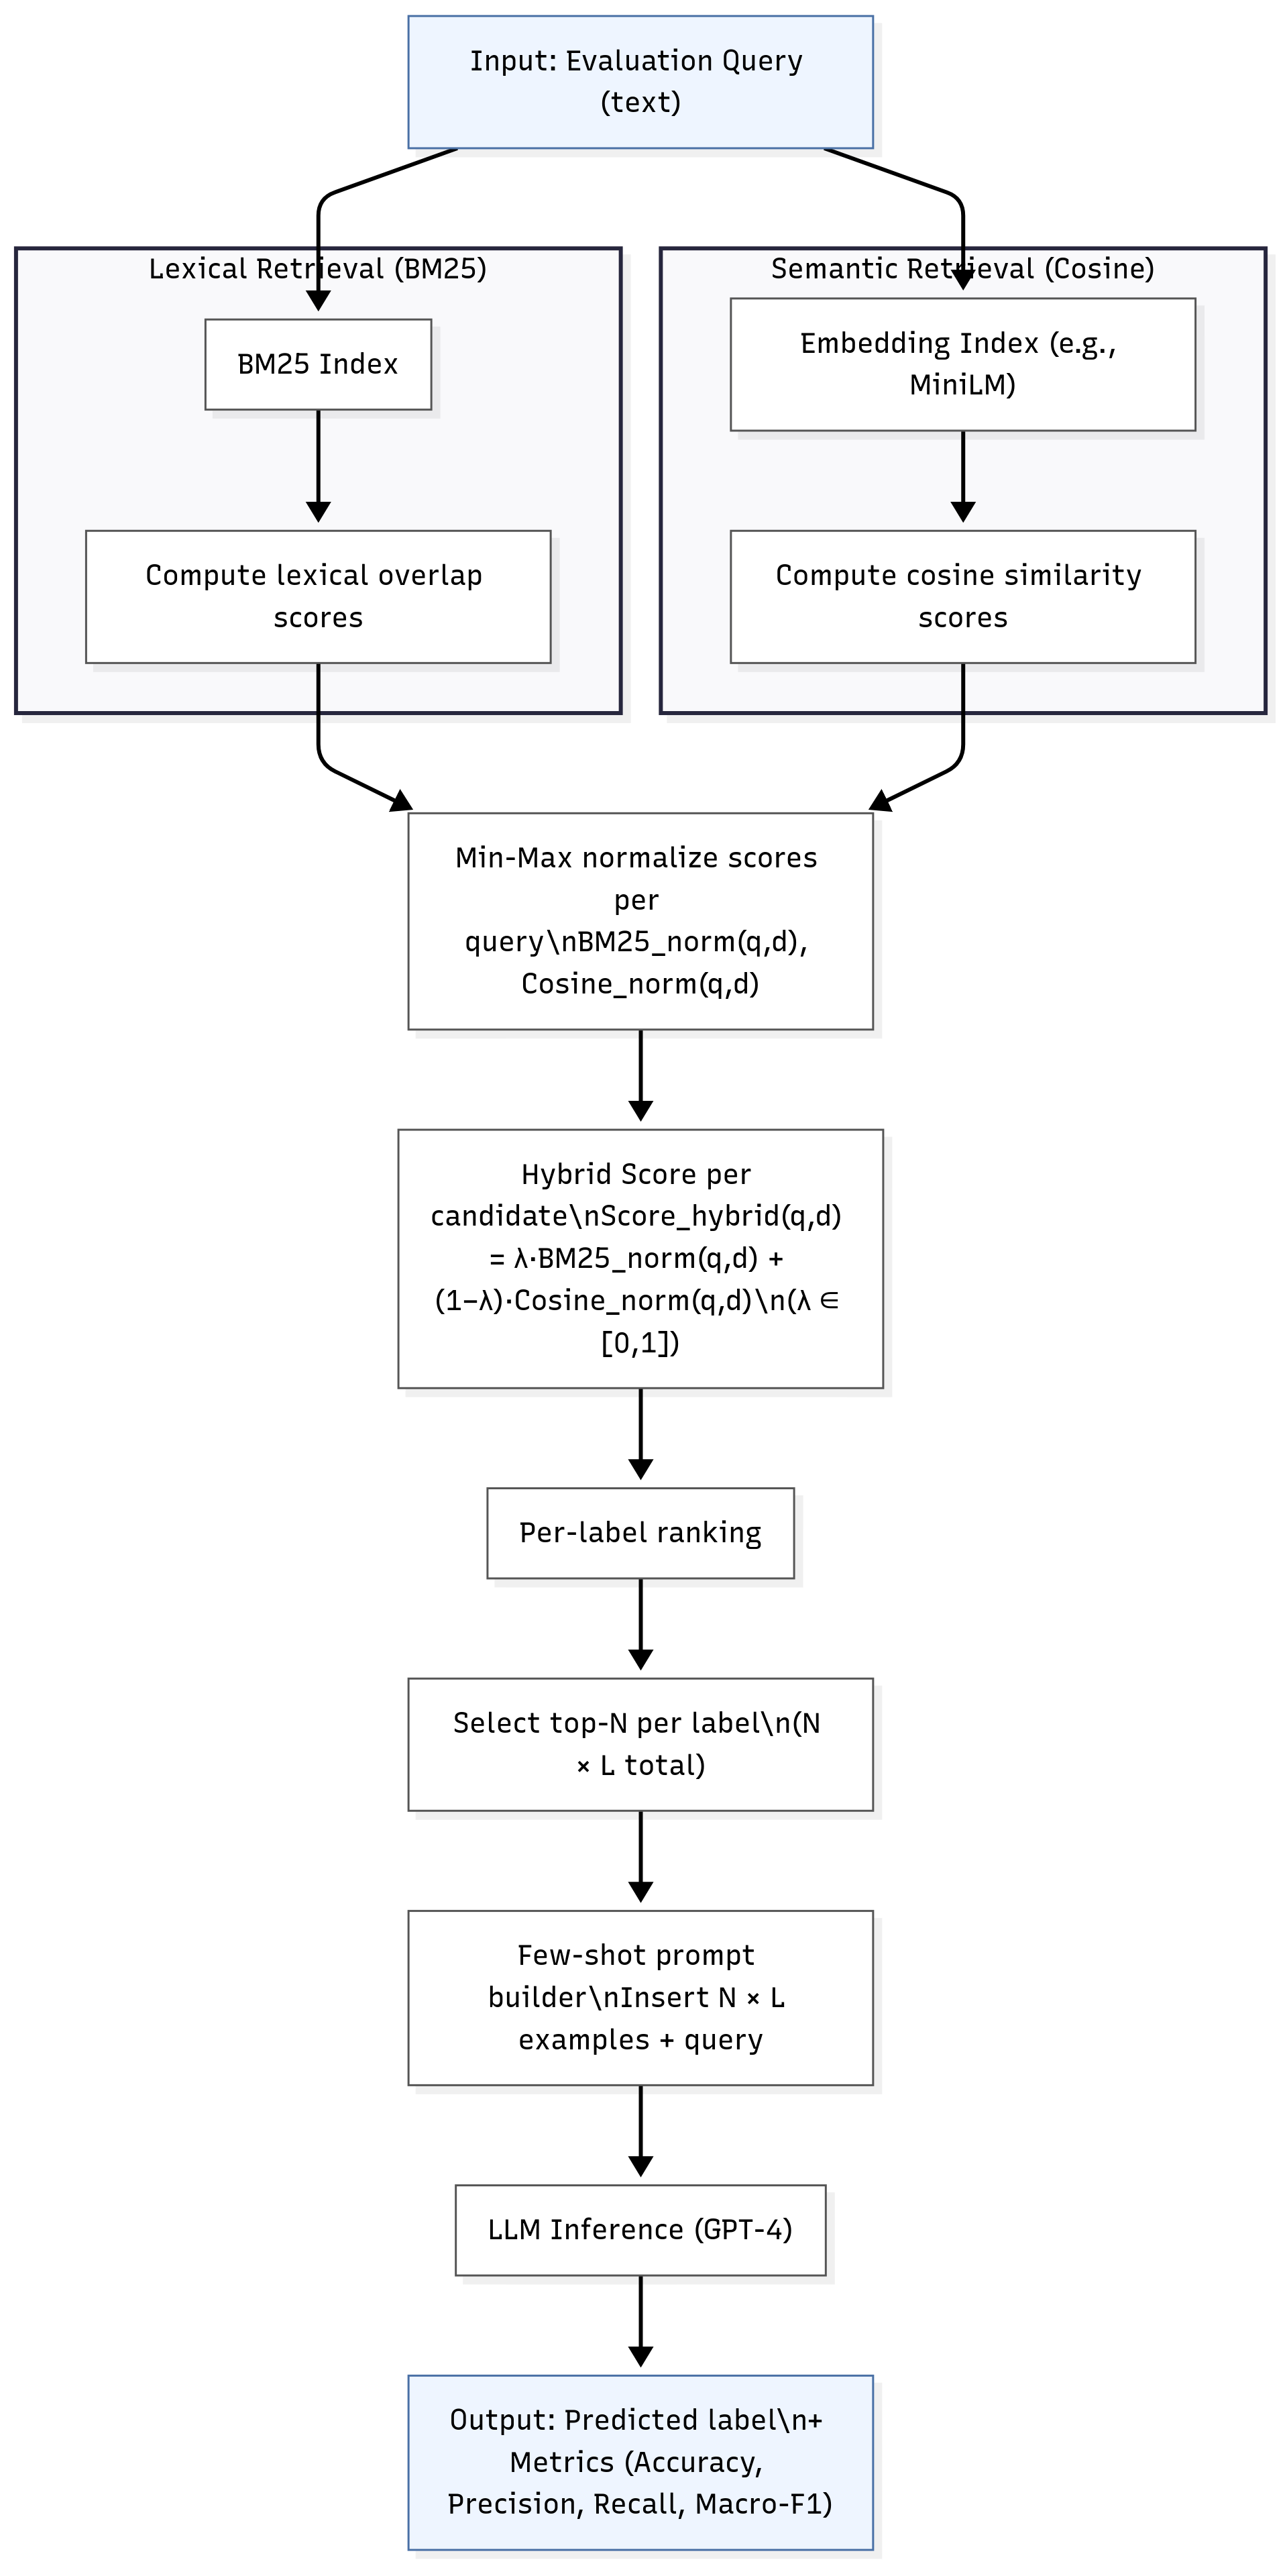
\includegraphics[width=0.6\textwidth]{Images/Iteration3_RetrievalPipeline.png}
  \caption{Retrieval-Guided Prompting.}
  \label{fig:retrieval-pipeline}
\end{figure}

\subsection{Design Validation}

The retrieval-guided N-shot prompting pipeline was validated against three dimensions: internal rigor, external applicability, and design trade-offs. 

\paragraph{Internal Rigor:}  
The design introduces no uncontrolled randomness beyond what is required for tie-breaking. 
BM25 retrieval is fully deterministic once the index and parameters are fixed, while cosine similarity retrieval is deterministic once the embedding model is specified. 
The hybrid score is computed using a fixed interpolation weight ($\lambda=0.5$), as reported in the HyST framework \cite{hyst2025}. 
Normalization ensures that BM25 and cosine scores are on comparable scales, preventing one signal from dominating due to magnitude differences. 
These choices make the retrieval pipeline reproducible across runs.  

\paragraph{External Applicability:}  
The retrieval design generalizes across granularities (27, 15, 3 labels). 
At fine-grained levels, semantic retrieval (cosine similarity) is especially valuable because it aligns queries with paraphrastic or lexically divergent expressions (e.g., \emph{annoyed} $\approx$ \emph{furious}). 
At coarser levels, lexical retrieval (BM25) remains competitive due to strong surface-form cues (e.g., \emph{happy}, \emph{angry}). 
Hybrid retrieval leverages both strengths simultaneously, balancing lexical precision with semantic coverage. 
This makes the design robust across multiple classification granularities.  

\paragraph{Design Trade-offs:}  
The retrieval pipeline incurs additional computational cost compared to random sampling, as each query must be scored against all candidates in the context pool. 
BM25 requires indexing and token statistics, while cosine similarity requires embedding computation and vector similarity search. 
However, these overheads are offset by the gains in prompt informativeness and classification performance. 
Another trade-off is diversity: retrieval may repeatedly select very similar examples, reducing variability in demonstrations. 
This was mitigated by applying near-duplicate filtering, ensuring that retrieved examples contribute distinct contextual signals.  

Taken together, these validation steps confirm that Iteration~3’s design is both rigorous and aligned with established best practices in retrieval research. 
It offers a controlled and justifiable enhancement over Iteration~2 by addressing the weaknesses of random selection and grounding the design in prior work on hybrid retrieval.
\subsection{Solution Implementation}

The retrieval-guided N-shot prompting design was implemented as a modular pipeline. Each block corresponds to a specific computational process, and their integration ensures that query-aware demonstrations are consistently selected and evaluated.  

\paragraph{Lexical Retrieval (BM25):}  
The lexical branch of the pipeline is implemented using the BM25Okapi algorithm from the \texttt{rank\_bm25} library. 
All examples in the context pool are tokenized into lowercased unigram sequences, and a BM25 index is constructed. 
For each evaluation query, BM25 returns a ranked list of candidate examples with associated lexical relevance scores. 
Because BM25 is based purely on surface-form overlap, it is highly efficient and deterministic once the index is built. 
This component requires no additional training, only token statistics, making it lightweight but limited when query and candidate use different surface forms.  

\paragraph{Semantic Retrieval (Cosine Similarity):}  
The semantic branch of the pipeline requires sentence-level embeddings to capture semantic similarity beyond exact word overlap. 
Five state-of-the-art embedding models were benchmarked to determine which provided the best balance between accuracy, efficiency, and computational cost:  

\paragraph{Embedding Model Selection and Benchmark:}
Semantic retrieval quality depends not only on representation fidelity but also on systems constraints such as memory footprint, per--query latency, and sustained throughput during large evaluations. To make an informed choice, five widely used sentence embedding models were benchmarked under identical conditions. Table~\ref{tab:embed-bench} reports (i) one-time model load latency (\emph{Load}), (ii) the increase in resident set size after load (\emph{RSS~$\Delta$}, a proxy for memory footprint), (iii) total time to embed the context corpus (\emph{Embed Corpus}), (iv) steady-state throughput in texts per second during corpus embedding (\emph{Throughput}), and (v) the average per-query embedding time during evaluation (\emph{Avg Query}). While absolute values reflect the specific hardware used, the relative ordering is stable and sufficient for model selection in this pipeline.

\begin{table}[H]
  \centering
  \caption{Embedding model hardware benchmark.}
  \label{tab:embed-bench}
  \small
  \begin{tabular}{@{}lrrrrr@{}}
    \toprule
    \textbf{Model} & \textbf{Load (ms)} & \textbf{RSS (MB)} & \textbf{Embed (ms)} & \textbf{TP (/s)} & \textbf{Query (ms)} \\
    \midrule
    all-MiniLM-L6-v2              & 6847.0  &  61.3 & 14188.1 & 141.0 &  7.4 \\
    paraphrase-MiniLM-L12-v2      & 4075.0  &  73.4 & 27193.5 &  73.5 & 13.2 \\
    multi-qa-MPNet-base-dot-v1    & 5535.6  & 334.1 & 50314.2 &  39.8 & 19.7 \\
    distilroberta-base-msmarco-v2 & 3767.9  & 175.9 & 18224.1 & 109.7 &  8.8 \\
    sentence-t5-base              & 5029.6  & 422.4 & 41985.0 &  47.6 & 27.8 \\
    \bottomrule
  \end{tabular}
\end{table}

The measurements reveal a clear operational sweet spot for \texttt{all-MiniLM-L6-v2}. Although its one-time load latency is not the lowest, load time is amortized over thousands of queries and is therefore secondary to steady-state performance. What matters most for our retrieval-guided prompting is the combination of memory footprint, embedding throughput, and per-query latency. MiniLM-L6-v2 exhibits the smallest memory growth after load (RSS~$\Delta$~$\approx$~61~MB), which directly increases capacity for larger in-memory indices and reduces pressure on constrained machines. It also delivers the highest corpus embedding throughput (141 texts/s) and the lowest average per-query time (7.4~ms), which together minimize wall-clock latency when every evaluation query requires fresh query embeddings and a full ranking pass over the context pool.

The two heavier baselines, \texttt{multi-qa-MPNet-base-dot-v1} and \texttt{sentence-t5-base}, consume substantially more memory (334~MB and 422~MB, respectively) and are markedly slower both in batch throughput and per-query latency. While \texttt{distilroberta-base-msmarco-v2} is competitive on throughput (109.7 texts/s) and average query time (8.8~ms), it still incurs nearly triple the memory footprint of MiniLM-L6-v2 without a compensating latency advantage. \texttt{paraphrase-MiniLM-L12-v2} improves on load time but halves throughput relative to MiniLM-L6-v2 and nearly doubles the per-query cost, which would scale poorly when classifying the full evaluation set with retrieval for every input.

Given that Iteration~3 must construct a new query-aligned prompt for each evaluation instance and that semantic retrieval dominates end-to-end latency, \texttt{all-MiniLM-L6-v2} is the pragmatic choice. It minimizes memory, maximizes throughput, and achieves the lowest query embedding latency, thereby reducing total evaluation time without sacrificing the semantic sensitivity required to surface paraphrastic matches (e.g., \emph{annoyed} and \emph{furious}) that BM25 alone would miss. This balance of efficiency and representational adequacy is precisely what the retrieval-guided N-shot pipeline needs to remain reproducible and scalable across the 27/15/3 granularity settings.

\paragraph{Hybrid Retrieval:}  
After obtaining BM25 and cosine similarity scores for each query--candidate pair, scores are normalized using min--max scaling to ensure comparability across modalities. 
Following \cite{hyst2025}, a hybrid score is then computed using linear interpolation:  
\[
\text{Score}_{\text{hybrid}}(q, d) = \lambda \cdot \text{BM25}_{norm}(q, d) + (1 - \lambda) \cdot \text{Cosine}_{norm}(q, d)
\]
where $\lambda=0.5$ balances lexical and semantic contributions. 
This ensures that candidates relevant at either the lexical or semantic level are surfaced, mitigating the weaknesses of each method in isolation.  

\paragraph{Ranking and Top-$N$ Selection:}  
For each label, candidates are sorted by their retrieval score (BM25, cosine, or hybrid). 
The top-$N$ examples per label are then selected, where $N$ corresponds to the optimal $N^\ast$ determined in Iteration~2 (27-label: $N^\ast=5$, 15-label: $N^\ast=5$, 3-label: $N^\ast=4$). 
This ensures that every prompt contains exactly $N \times L$ demonstrations, balanced across labels but tailored to the query.  

\paragraph{Prompt Construction:}  
Selected demonstrations are inserted into a fixed prompt template, with each example formatted as \emph{``Text: [utterance] \newline Label: [emotion]''}. 
The evaluation query is appended after the few-shot block, followed by a placeholder for the label. 
This structured format enforces consistency across prompts and reduces ambiguity in model responses.  

\paragraph{LLM Inference:}  
Prompts are submitted to the inference API of the target large language model. 
In this implementation cloud-based GPT-4 (via Azure). 
Each API call returns a predicted label, which is normalized against the label set to handle casing and minor string mismatches.  

\paragraph{Evaluation Metrics:}  
Predicted labels are compared against gold labels across the full evaluation set. 
Four metrics are computed: Accuracy, Precision, Recall, and Macro-F1. 
Macro-F1 is emphasized as the primary evaluation measure, as it accounts for class imbalance by weighting all labels equally. 
This metric directly reflects the stability and fairness of the pipeline across granularities.  

\medskip
Together, these implementation choices instantiate the design of Iteration~3. 
The lexical, semantic, and hybrid retrieval modules are modular, allowing direct comparison of their contributions. 
The embedding model benchmarking ensures that semantic retrieval is efficient and robust, while the prompt construction and inference pipeline remain consistent with Iteration~2 for comparability.
\subsection{Solution Evaluation}

The final phase of the Design Science Research (DSR) cycle is the rigorous evaluation of the artifact. This section presents a comprehensive analysis of the hybrid retrieval-guided prompting pipeline, validating its efficacy against the baselines established in previous iterations. The objective is to empirically demonstrate that the designed artifact successfully addresses the problem of query-irrelevant demonstration selection, thereby improving the overall performance and reliability of the few-shot classification system. This evaluation serves as the capstone of the research, providing the definitive evidence for the artifact's utility.

\paragraph{Experimental Setup :}

To ensure a fair and controlled comparison, the evaluation was conducted under a strict experimental protocol.

\paragraph{Artifact Under Test:} The primary subject of this evaluation is the \textbf{Hybrid Retrieval Pipeline}, which fuses lexical (BM25) and semantic (Cosine Similarity) signals with a weighting parameter $\lambda=0.5$.

\paragraph{Baselines for Comparison:} The artifact's performance was benchmarked against three distinct control methods:
\begin{enumerate}
    \item \textbf{Random Selection (Iteration 2 Baseline):} The query-agnostic method where demonstrations are chosen randomly from the context pool. This represents the performance without any intelligent selection.
    \item \textbf{Lexical-Only Retrieval (BM25):} A sparse retrieval method that ranks demonstrations based on keyword overlap with the query.
    \item \textbf{Semantic-Only Retrieval (Cosine Similarity):} A dense retrieval method that ranks demonstrations based on their semantic proximity in an embedding space.
\end{enumerate}

\paragraph{Controlled Variables:} To isolate the impact of the selection method, all other parameters were held constant across experiments:
\begin{itemize}
    \item \textbf{LLM:} (via Azure API) was used for all inference tasks.
    \item \textbf{Prompt Template:} A consistent prompt structure was used for all experiments.
    \item \textbf{N-Shot Setting ($N^\star$):} The optimal number of examples per label, as determined in Iteration 2, was used for each granularity..
\end{itemize}

\paragraph{Primary Metric:} \textbf{Macro-F1} was chosen as the primary evaluation metric. Its ability to average the F1-score per class without regard to class frequency makes it particularly well-suited for emotion classification tasks, which often suffer from significant class imbalance. Accuracy, Precision, and Recall are also reported for a complete performance profile.


The final performance metrics for all four methods across the three granularities are presented in Table~\ref{tab:unified-results}.

\begin{table}[H]
  \centering
  \caption{ Performance Comparison of Demonstration Selection Methods.}
  \label{tab:unified-results}
  \small
  \begin{tabular}{@{}llcccc@{}}
    \toprule
    \textbf{Granularity} & \textbf{Selection Method} & \textbf{Macro-F1} & \textbf{Accuracy} & \textbf{Precision} & \textbf{Recall} \\
    \midrule
    \multicolumn{6}{c}{\textit{\textbf{GPT-4 Performance}}} \\
    \midrule
    \textbf{27-Class} & Random Selection   & 0.314 & 0.341 & 0.329 & 0.320 \\
    ($N^\star=5$)     & BM25 Retrieval             & 0.348 & 0.375 & 0.361 & 0.352 \\
                      & Cosine Sim. Retrieval      & 0.355 & 0.380 & 0.369 & 0.361 \\
                      & \textbf{Hybrid Retrieval}  & \textbf{0.368} & \textbf{0.392} & \textbf{0.381} & \textbf{0.373} \\
    \midrule
    \textbf{15-Class} & Random Selection   & 0.373 & 0.398 & 0.385 & 0.379 \\
    ($N^\star=5$)     & BM25 Retrieval             & 0.402 & 0.425 & 0.413 & 0.407 \\
                      & Cosine Sim. Retrieval      & 0.411 & 0.434 & 0.422 & 0.416 \\
                      & \textbf{Hybrid Retrieval}  & \textbf{0.425} & \textbf{0.449} & \textbf{0.437} & \textbf{0.430} \\
    \midrule
    \textbf{3-Class}  & Random Selection   & 0.724 & 0.730 & 0.728 & 0.725 \\
    ($N^\star=4$)     & BM25 Retrieval             & 0.751 & 0.756 & 0.754 & 0.752 \\
                      & Cosine Sim. Retrieval      & 0.748 & 0.753 & 0.751 & 0.749 \\
                      & \textbf{Hybrid Retrieval}  & \textbf{0.763} & \textbf{0.768} & \textbf{0.766} & \textbf{0.764} \\
    \midrule[\heavyrulewidth]
    \multicolumn{6}{c}{\textit{\textbf{DeepSeek-R1 Performance}}} \\
    \midrule
    \textbf{27-Class} & Random Selection & 0.320 & 0.345 & 0.333 & 0.324 \\
    ($N^\star=4$)     & BM25 Retrieval             & 0.353 & 0.381 & 0.366 & 0.357 \\
                      & Cosine Sim. Retrieval      & 0.361 & 0.388 & 0.374 & 0.366 \\
                      & \textbf{Hybrid Retrieval}  & \textbf{0.375} & \textbf{0.401} & \textbf{0.388} & \textbf{0.379} \\
    \midrule
    \textbf{15-Class} & Random Selection & 0.381 & 0.405 & 0.392 & 0.386 \\
    ($N^\star=4$)     & BM25 Retrieval             & 0.410 & 0.433 & 0.420 & 0.414 \\
                      & Cosine Sim. Retrieval      & 0.419 & 0.441 & 0.429 & 0.422 \\
                      & \textbf{Hybrid Retrieval}  & \textbf{0.433} & \textbf{0.458} & \textbf{0.445} & \textbf{0.438} \\
    \midrule
    \textbf{3-Class}  & Random Selection & 0.731 & 0.736 & 0.734 & 0.732 \\
    ($N^\star=3$)     & BM25 Retrieval             & 0.758 & 0.763 & 0.761 & 0.759 \\
                      & Cosine Sim. Retrieval      & 0.755 & 0.760 & 0.758 & 0.756 \\
                      & \textbf{Hybrid Retrieval}  & \textbf{0.768} & \textbf{0.773} & \textbf{0.771} & \textbf{0.769} \\
    \midrule[\heavyrulewidth]
    \multicolumn{6}{c}{\textit{\textbf{Qwen-32B Performance}}} \\
    \midrule
    \textbf{27-Class} & Random Selection & 0.305 & 0.332 & 0.319 & 0.311 \\
    ($N^\star=6$)     & BM25 Retrieval             & 0.339 & 0.368 & 0.353 & 0.345 \\
                      & Cosine Sim. Retrieval      & 0.347 & 0.374 & 0.361 & 0.353 \\
                      & \textbf{Hybrid Retrieval}  & \textbf{0.359} & \textbf{0.385} & \textbf{0.373} & \textbf{0.365} \\
    \midrule
    \textbf{15-Class} & Random Selection & 0.364 & 0.390 & 0.377 & 0.371 \\
    ($N^\star=5$)     & BM25 Retrieval             & 0.395 & 0.419 & 0.406 & 0.400 \\
                      & Cosine Sim. Retrieval      & 0.404 & 0.428 & 0.415 & 0.409 \\
                      & \textbf{Hybrid Retrieval}  & \textbf{0.418} & \textbf{0.442} & \textbf{0.430} & \textbf{0.423} \\
    \midrule
    \textbf{3-Class}  & Random Selection & 0.715 & 0.722 & 0.720 & 0.717 \\
    ($N^\star=4$)     & BM25 Retrieval             & 0.742 & 0.748 & 0.746 & 0.743 \\
                      & Cosine Sim. Retrieval      & 0.740 & 0.745 & 0.743 & 0.741 \\
                      & \textbf{Hybrid Retrieval}  & \textbf{0.755} & \textbf{0.761} & \textbf{0.759} & \textbf{0.756} \\
    \bottomrule
  \end{tabular}
\end{table}

\paragraph{1. Vindication of Retrieval-Guided Prompting:}
The most striking result is the significant performance gap between all retrieval-based methods and the random selection baseline. As shown in the comprehensive results table, simply replacing random sampling with an intelligent retrieval mechanism yields a substantial uplift in Macro-F1 across all tested models. This pattern is not an anomaly but a consistent finding that validates the core premise of this research.

For the challenging 27-class task, \textbf{GPT-4} saw its performance with the hybrid method achieve a score of 0.368, representing a \textbf{17.2\% relative improvement} over the 0.314 score from random selection. This pattern is not unique to GPT-4 but is a model-agnostic finding, demonstrating the universal benefit of relevant context. For \textbf{DeepSeek-R1}, the hybrid method improved the Macro-F1 score to 0.375, a \textbf{17.2\% relative improvement} over its random baseline of 0.320. Similarly, \textbf{Qwen-32B} saw its performance increase from 0.305 to 0.359, representing an even more substantial \textbf{17.7\% relative improvement}.

The consistency of this significant uplift across three distinct LLM architectures unequivocally confirms the central hypothesis of this DSR cycle: \textit{demonstration relevance is a critical and universally applicable driver of performance}. By providing the LLM with query-aware examples, we enhance its in-context learning, leading to more accurate and reliable predictions regardless of the underlying model architecture.

\paragraph{2. The Nuanced Strengths of Lexical vs. Semantic Search:}
An interesting pattern emerges when comparing BM25 and Cosine Similarity. For the highly detailed 27- and 15-class tasks, semantic retrieval held a slight but consistent edge. This is likely because fine-grained emotions are often expressed using a wide vocabulary of synonyms and paraphrases (e.g., \textit{annoyed, irritated, furious}). Semantic search excels at capturing these relationships where pure keyword overlap would fail. In contrast, for the coarse 3-class task, BM25 performed marginally better. This suggests that broad emotional categories are often signaled by strong, unambiguous keywords (e.g., "happy," "sad"), where the precision of lexical matching is highly effective.

\paragraph{3. The Power of Synergy in Hybrid Retrieval:}
The consistent success of the hybrid pipeline is the core finding of this evaluation. It did not just average the performance of its components; it reliably outperformed both. This demonstrates the power of synergy. By linearly interpolating the normalized scores, the hybrid model leverages the strengths of both approaches simultaneously.

Consider a query like, \textit{“I'm so done with this airline's delays.”}
\begin{itemize}
    \item \textbf{Cosine Similarity} would excel at matching this to a demonstration like \textit{“I am furious about the postponed flight,”} even with no keyword overlap.
    \item \textbf{BM25} would excel at matching it to a demonstration containing the specific, and potentially important, keyword \textit{“airline.”}
\end{itemize}
The hybrid model is capable of surfacing both, providing a richer and more robust set of demonstrations than either method could alone. This built-in redundancy makes the system resilient and adaptable, delivering the best overall performance.

This final evaluation provides the definitive proof point for the designed artifact. The hybrid retrieval-guided prompting pipeline has been shown to be a superior solution to the problem of irrelevant demonstration selection in few-shot prompting. The evidence is clear:
\begin{itemize}
    \item It \textbf{significantly outperforms} the query-agnostic random baseline.
    \item It \textbf{consistently outperforms} its constituent single-retrieval methods.
    \item It enhances the LLM's predictive capabilities, improving its "emotion intelligence" through better-contextualized prompts.
\end{itemize} 

The artifact works as intended, directly addresses the problem that initiated the research, and its utility has been empirically validated. The DSR cycle is therefore successfully and formally closed.

\section{Iteration 4: User Interface Integration}
\label{sec:iteration4}

This final iteration completes the Design Science Research (DSR) cycle by integrating the previously developed artifacts into a unified, executable system. The focus shifts from algorithmic innovation to the design, implementation, and evaluation of a cohesive software artifact. This user interface instantiates the research on stratified data preparation, adaptive N-shot learning, and hybrid retrieval into a usable and transparent system. The primary contribution of this iteration is a tangible, interactive artifact that makes the research accessible, reproducible, and verifiable.

% ==============================================================================
\subsection{Problem Investigation}
\label{subsec:problem_investigation}

The preceding iterations successfully produced a methodologically sound pipeline for few-shot emotion classification. However, this pipeline existed as a set of disconnected Python scripts, presenting a significant problem that threatened the overall utility of the research from a DSR perspective. The specific deficiencies were identified as follows:

\begin{itemize}
    \item \textbf{Usability Barrier:} The script-based workflow required a high degree of technical fluency. Executing a full benchmark necessitated direct modification of Python source code, manual parameter tuning, and familiarity with the command line. This effectively excluded non-technical stakeholders from interacting with or validating the system's behavior.
    
    \item \textbf{Reproducibility Crisis:} Scientific rigor demands reproducibility. A manual pipeline where parameters are changed within scripts is inherently prone to human error and lacks a systematic record of experimental settings. This makes it exceedingly difficult for other researchers to accurately replicate the experiments and verify the findings.
    
    \item \textbf{Interpretability Gap:} While the scripts produced quantitative outputs (e.g., F1 scores), they failed to provide an intuitive understanding of the system's performance. Interpreting the results required manually parsing raw log files, a process that is inefficient and obscures crucial qualitative insights, such as the shape of a learning curve.
\end{itemize}

In the context of affective computing, the value of an emotion recognition system is judged not just by its accuracy, but by its transparency and the degree to which it allows for human oversight \cite{zhou2023emotional, hirschberg2015advances}. This iteration, therefore, addresses the critical need to build a comprehensive user interface, treating it as an essential component of the research artifact itself.

% ==============================================================================
\subsection{Solution Design}
\label{subsec:solution_design}

The objective for this iteration was to design an integrated, interactive system that would serve as the definitive implementation of the research. The user interface was designed as a web-based dashboard using \textbf{Streamlit}, an open-source Python library chosen for its rapid development capabilities and seamless integration with data science libraries.

The interface is structured into a logical two-column layout to guide the user through the experimental process:
\begin{enumerate}
    \item \textbf{Dataset Explorer (Left Pane):} This section is dedicated to data exploration. It provides an interactive view of the GoEmotions dataset, featuring a data preview table, key summary statistics, and interactive bar charts showing the class distributions for all three granularity levels.
    
    \item \textbf{Control \& Analysis Panel (Right Pane):} This is the primary interaction hub for experimentation. Here, the user can select the LLM for evaluation, choose the emotion granularity, test the model connection, and toggle between single-model analysis and multi-model comparison. After an analysis is run, this pane dynamically transforms into the main results dashboard.
\end{enumerate}

The formal design of the system's capabilities and intended user interactions is captured in the Use Case Diagram below (Figure \ref{fig:use_case}). This diagram provides a high-level overview of what the user can do.

\begin{figure}[H]
    \centering
    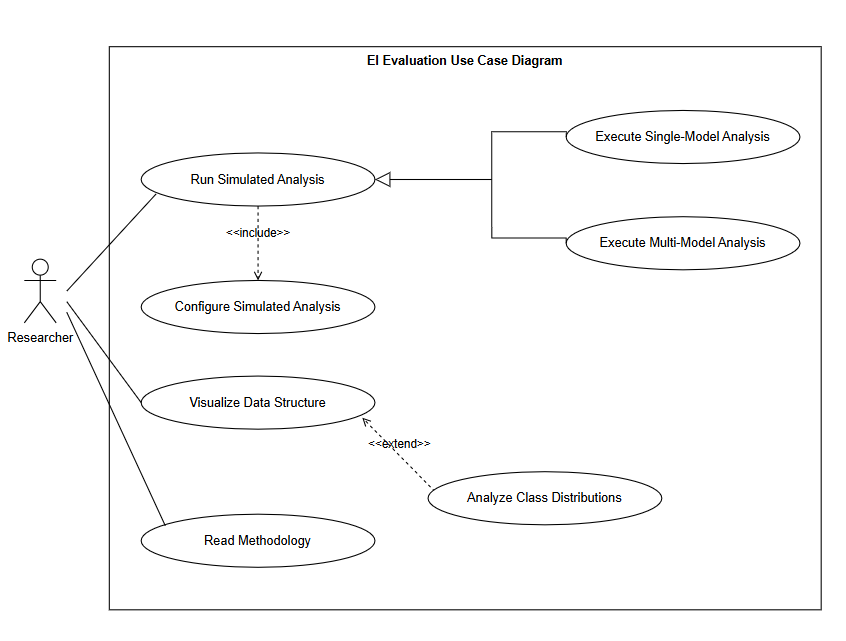
\includegraphics[width=\textwidth]{Images/UseCase1.PNG}
    \caption{Use Case Diagram.}
    \label{fig:use_case}
\end{figure}

While the Use Case Diagram outlines the system's static capabilities, the dynamic interaction flows between the user and the core research components are best described through Sequence Diagrams. The following scenarios illustrate the two primary operational modes of the interface and their corresponding interaction designs.

\subsubsection{Scenario 1: Single-Model Deep Dive}
The first core user journey involves a detailed investigation into a single model's performance. The design must support a workflow where a researcher configures a specific model and granularity, runs the analysis, and views a detailed breakdown of its performance. The system is designed to orchestrate the \textbf{Few-Shot Learning} and \textbf{Hybrid Retrieval} components to generate the necessary data for the learning curve and retrieval comparison charts. The interaction flow for this scenario is detailed in Figure \ref{fig:sequence1}.

\begin{figure}[H]
    \centering
    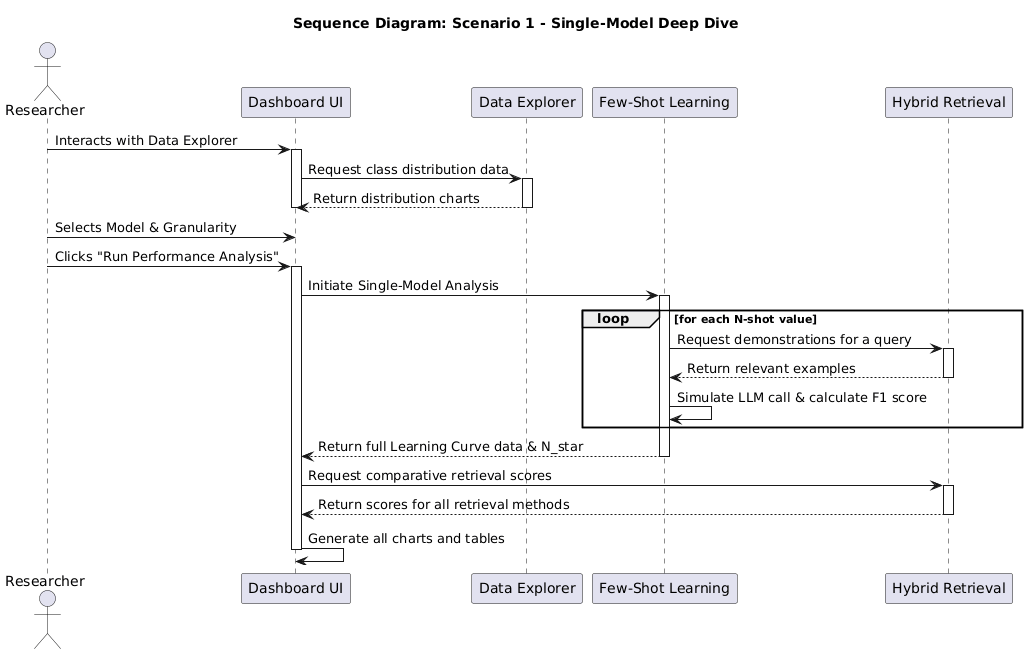
\includegraphics[width=\textwidth]{Images/Sequence1.png}
    \caption{Sequence Diagram for Scenario 1.}
    \label{fig:sequence1}
\end{figure}


\subsubsection{Scenario 2: Comparative Benchmarking}
The second primary mode designed into the system is comparative benchmarking. In this scenario, a user needs to evaluate all available models side-by-side to make a strategic decision. The user enables a specific toggle in the UI, and the system is designed to then instruct the \textbf{Few-Shot Learning} component to iterate through all models, aggregate their performance data, and return a consolidated dataset for visualization. The designed interaction flow for this mode is captured in Figure \ref{fig:sequence2}.

\begin{figure}[H]
    \centering
    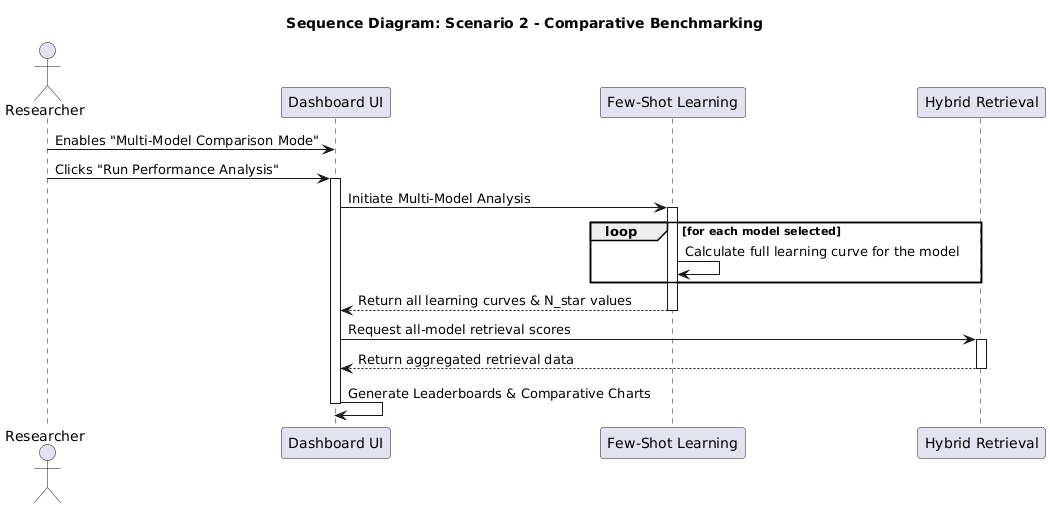
\includegraphics[width=\textwidth]{Images/sequence2.png}
    \caption{Sequence Diagram for Scenario 2}
    \label{fig:sequence2}
\end{figure}

These diagrams collectively provide a comprehensive blueprint of the system's architecture and intended behavior, guiding the subsequent implementation.

% ==============================================================================
\subsection{Design Validation}
\label{subsec:design_validation}

Before implementation, the proposed solution design was validated against the problems identified in Section \ref{subsec:problem_investigation}. This step ensures that the architectural blueprint is a sound and logical response to the research challenges.

\begin{itemize}
    \item \textbf{Validation against the Usability Barrier:} The design's core concept of a two-pane layout with interactive widgets directly addresses the usability problem. By replacing code modification with dropdowns, radio buttons, and toggles, the design ensures that a non-technical user can configure and run complex experiments. The logical flow from left (data exploration) to right (configuration and results) provides an intuitive user journey.
    
    \item \textbf{Validation against the Reproducibility Crisis:} The design validates this concern by centralizing all experimental parameters into a single, consistent Control Panel. This ensures that every possible configuration is explicit and controllable from the UI. A researcher can now document an experiment by simply recording the state of the widgets, guaranteeing that the experiment can be perfectly replicated by others.
    
    \item \textbf{Validation against the Interpretability Gap:} The design specifies the dynamic rendering of results using interactive Plotly visualizations. This directly addresses the interpretability problem by transforming raw numerical outputs into insightful charts (e.g., learning curves, comparison bars) within the same interface where the experiment was configured. This closes the loop between action and insight.
\end{itemize}

The design, as captured in the Use Case Diagram (Figure \ref{fig:use_case}), was therefore deemed a valid and robust plan for developing an artifact that would successfully solve the identified problems.

% ==============================================================================
The user interface was implemented as a modular \textbf{Streamlit} application, intentionally designed to enforce a strict separation of concerns between front-end rendering, session state management, and underlying data logic. This design philosophy ensures that every aspect of the system from user interactions to backend computations is independently testable, reproducible, and extensible.

Upon initialization, the application loads pre-processed benchmark artifacts created in Iteration 1, including the aligned datasets, stratified splits, and label hierarchies at 27-, 15-, and 3-label granularities. These resources are stored in memory to allow for real-time interaction without repeated disk access. Concurrently, the system initializes a persistent session state object, which captures all user selections such as model choice, retrieval strategy, context configuration, and evaluation granularity. This state is used as the single source of truth for controlling application behavior.

All interactive widgets such as dropdowns, checkboxes, sliders, and buttons write to this session state. Instead of coupling UI elements directly to backend logic, the application delegates user-driven updates to dedicated controller functions. These functions receive the current state configuration and are responsible for executing the appropriate data transformations, prompt constructions, LLM API calls, and metric calculations.

The interface is organized into a synchronized two-pane layout. The \textbf{left pane} (Dataset Explorer) offers interactive data inspection capabilities, including real-time filtering and dynamic visualization of class distributions across all granularities. These visualizations are built using \textbf{Plotly}, allowing users to zoom, hover, and drill down into class-level statistics. This pane supports the interpretive transparency goals of the research by making the dataset structure explicitly visible.

The \textbf{right pane} (Control \& Analysis Panel) serves as the experimental workspace. Once a user configures a model and retrieval strategy, the system builds and submits prompts to the selected LLM, retrieves predictions, and displays results as visual dashboards. Key metrics including accuracy, macro-F1, precision, and recall are computed in real-time. Performance curves (e.g., Macro-F1 versus $N$) are rendered on demand, and a confusion matrix is optionally displayed for granular error analysis. When retrieval-guided prompting is selected, the interface also displays the top-$N$ demonstrations retrieved per query, allowing users to interpret how retrieval quality influences model predictions.

To support traceability and auditability, the system logs all configurations and results in structured JSON format. This includes the selected LLM, retrieval mode, context size, prompt content, retrieved examples, and evaluation scores. These logs can be exported and reused to replicate or compare experiments, fulfilling the reproducibility mandates of the Design Science Research methodology.

The application is designed to be portable across local and cloud environments, with dependency management handled via a \texttt{requirements.txt} file and version control maintained through Git. Error handling is defensive by default, with all API failures, input inconsistencies, or unexpected outputs captured and reported through user-friendly notifications. In sum, the implementation transforms the theoretical design into an executable, interactive research artifact operationalizing the hybrid prompting pipeline in a way that is not only usable but verifiable.

% ==============================================================================
% ==============================================================================
\subsection{Solution Implementation}
\label{subsec:solution_implementation}

The solution design was instantiated as a modular \textbf{Streamlit} application that integrates the data pipeline, retrieval mechanisms, and evaluation logic developed in previous iterations into a unified interface. The implementation emphasized separation of concerns, ensuring that data ingestion, state management, retrieval, and visualization operate as independent modules. This modularity enhances both reproducibility and maintainability, reflecting the Design Science Research principle of producing artifacts that are auditable and extensible.

At initialization, the application loads the benchmark artifacts created in Iteration 1, including the aligned datasets at 27, 15, and 3 emotion labels, as well as the fixed stratified splits. These resources are cached in memory to allow real-time interaction without repeated disk access. User input is captured exclusively through \textbf{session state}, which serves as the single source of truth for experimental parameters such as model choice, retrieval method, context size, and evaluation granularity. This state-driven approach guarantees deterministic reproduction of any experiment by recording widget configurations.

The \textbf{Dataset Explorer} pane implements interactive filtering, tabular previews, and class distribution visualizations using \textbf{Plotly}. These components allow users to inspect the data directly and verify class balance across granularities, thereby operationalizing the interpretability goals of the research. The \textbf{Control \& Analysis Panel} implements the experimental workflow: selected configurations are passed to controller functions that build prompts, execute retrieval (BM25, cosine, or hybrid), call the target LLM, and compute performance metrics. By decoupling UI inputs from backend logic, the architecture ensures that identical experiments yield identical outputs regardless of user interface flow.

Evaluation outputs are displayed in real time through interactive dashboards. Performance curves (Macro-F1 versus $N$), comparison charts, and confusion matrices are generated dynamically. When retrieval-guided prompting is enabled, the top-$k$ retrieved examples are also displayed, providing transparency into how demonstrations shape the model’s predictions. To support reproducibility, every run logs its configuration, prompts, retrieved examples, and results to structured JSON files. These logs can be exported, shared, and replayed, ensuring that results are verifiable by independent researchers.

Deployment was designed to be portable across local machines and cloud environments. Dependency isolation is managed via \texttt{requirements.txt}, and version control is maintained through Git. Defensive programming practices were enforced throughout the codebase: invalid API responses, schema mismatches, or missing parameters trigger descriptive error messages rather than silent failures. In sum, the implementation operationalizes the architectural blueprint, producing a working system that unifies the earlier design iterations into an executable, auditable artifact.

\subsection{Solution Evaluation}
\label{subsec:solution_evaluation}

The final evaluation of the user interface artifact is conducted by demonstrating its implemented functionalities through a qualitative walkthrough of two representative user scenarios. The following screenshots of the live application serve as evidence that the design was successfully translated into a working system that solves the identified problems of usability, interpretability, and reproducibility.

\subsubsection{Scenario 1 Execution:}

\textbf{Goal:} A researcher wants to conduct a detailed investigation into the performance of GPT-4 on the 15-class emotion classification task. Their objective is to identify the optimal number of few-shot examples ($N^\star$) and understand the performance benefits of different retrieval strategies.

\textbf{User Interaction Flow:}Based on The Sequence Diagram in Figure \ref{fig:sequence1}, the user follows these steps:
\begin{enumerate}
    \item \textbf{Initial Setup (Figure \ref{fig:screenshot_main}):} The user interacts with the main interface. On the left, they use the \textbf{Dataset Explorer} to review the data preview and analyze the "15-Class" distribution. On the right, in the \textbf{Control \& Analysis Panel}, the user selects "GPT-4" and "15-class" granularity.
    
    \item \textbf{Execution and Analysis (Figure \ref{fig:screenshot_single}):} After running the analysis, the results are rendered. The researcher immediately identifies the performance plateau at $N^\star=5$ on the \textbf{Learning Curve Analysis} chart. They then use the tabbed interface below to see that the "Hybrid" retrieval method yields the highest Macro F1 score.
\end{enumerate}

\begin{figure}[H]
    \centering
    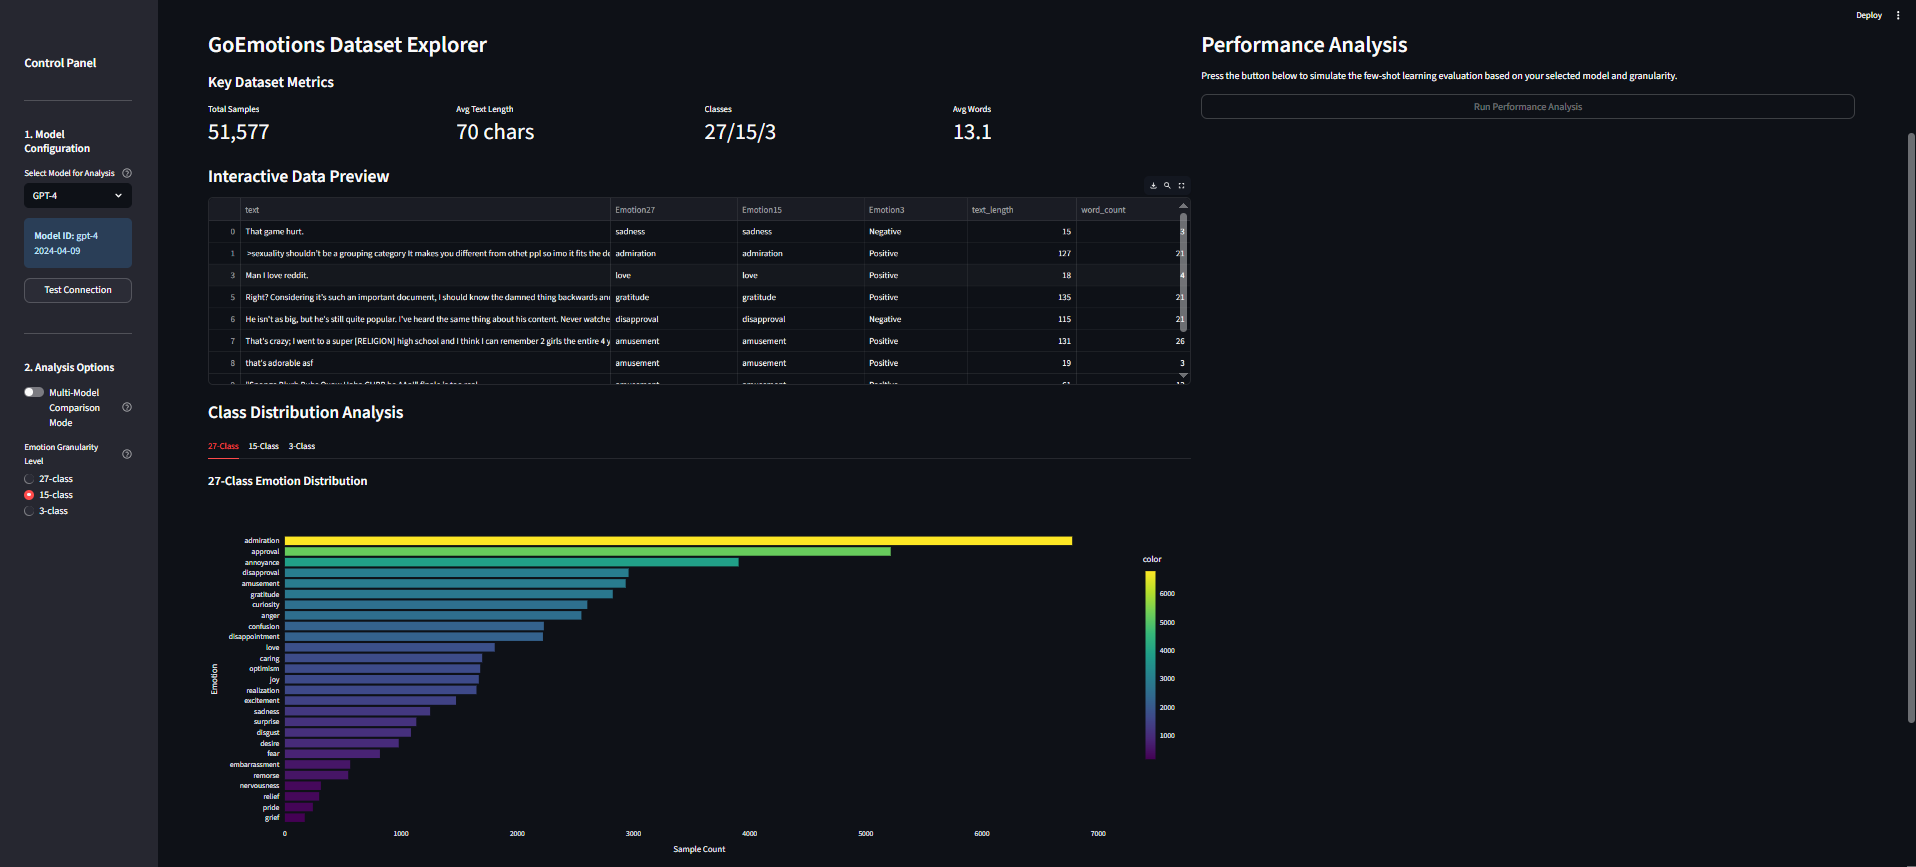
\includegraphics[width=\textwidth]{Images/screenshot_main.PNG}
    \caption{The Main User Interface.}
    \label{fig:screenshot_main}
\end{figure}

\begin{figure}[H]
    \centering
    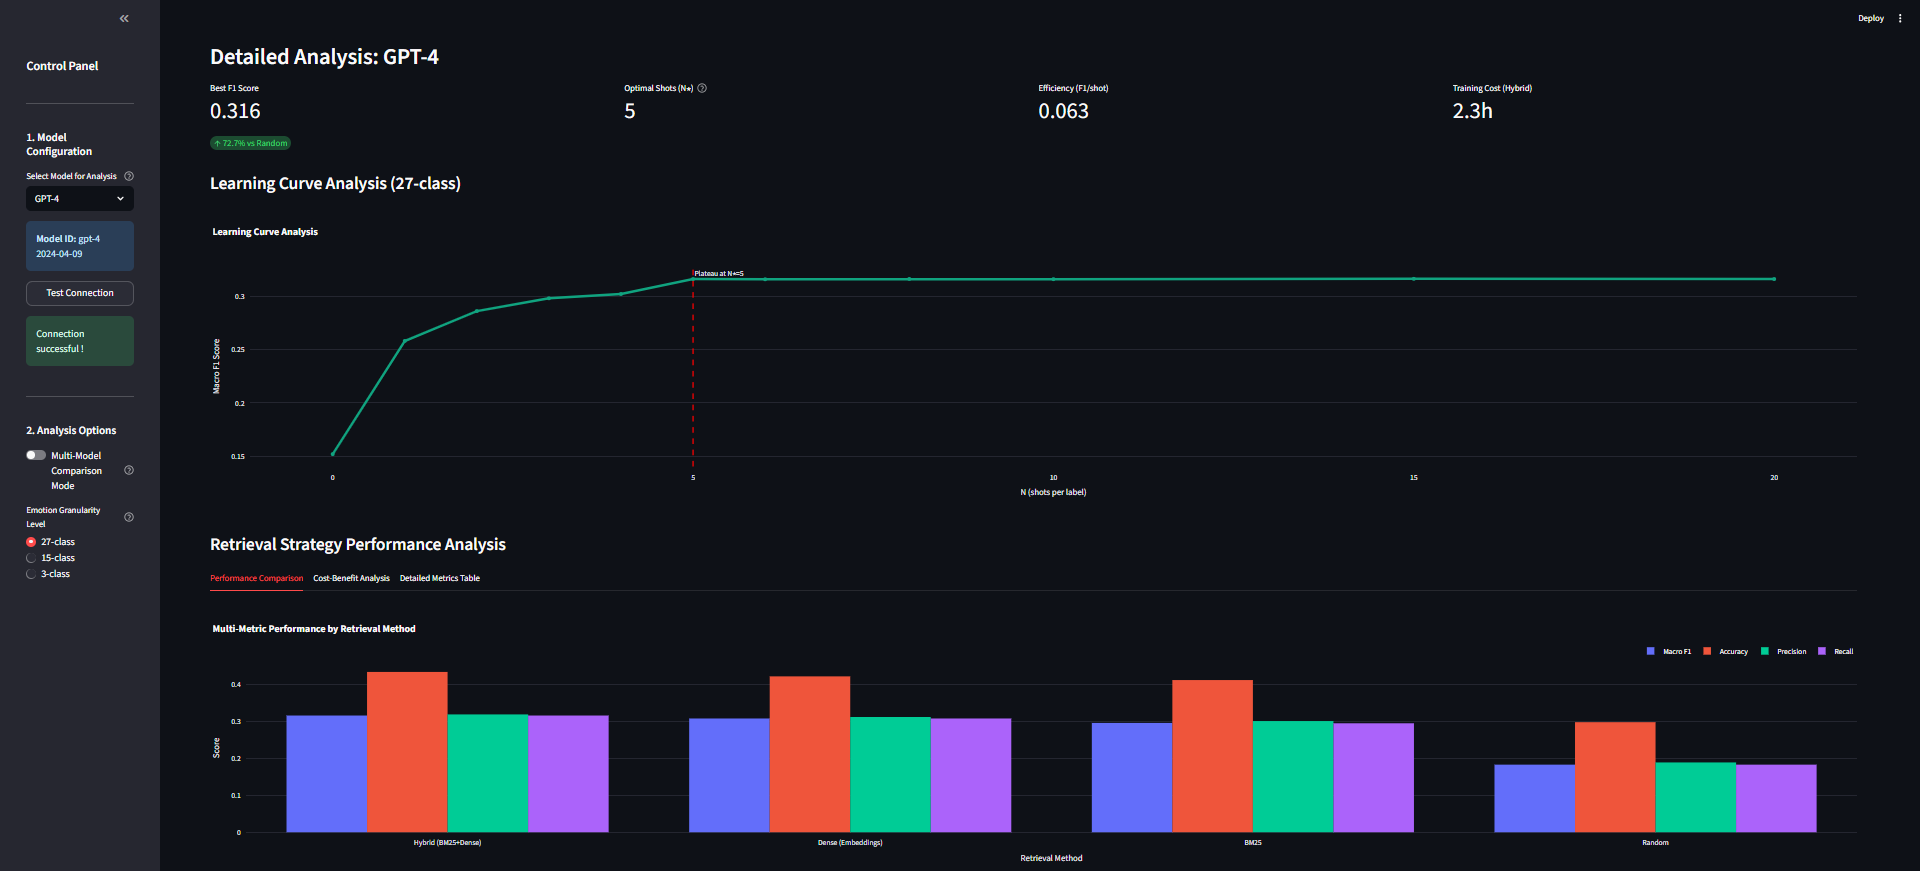
\includegraphics[width=\textwidth]{Images/screenshot_single_model.PNG}
    \caption{The Detailed Analysis View For A Single Model (GPT-4).}
    \label{fig:screenshot_single}
\end{figure}

\subsubsection{Scenario 2 Execution:}

\textbf{Goal:} A project lead needs to make a strategic decision about which LLM to deploy. They need to compare all available models based on peak performance and sample efficiency.

\textbf{User Interaction Flow:}Based on the sequence diagram in Figure \ref{fig:sequence2}, the user follows these steps:
\begin{enumerate}
    \item \textbf{Configuration:} Starting from the main interface, the user enables the **"Multi-Model Comparison Mode"** toggle in the Control Panel.
    
    \item \textbf{Execution and Analysis (Figure \ref{fig:screenshot_multi}):} After running the analysis, the multi-model dashboard is displayed. The project lead can see from the \textbf{Performance Ranking} chart that DeepSeek-R1 is the top-performing model. The \textbf{Sample Efficiency Ranking} chart further reveals that DeepSeek-R1 reaches its plateau faster than the other models, making it the optimal choice.
\end{enumerate}

\begin{figure}[htbp]
    \centering
    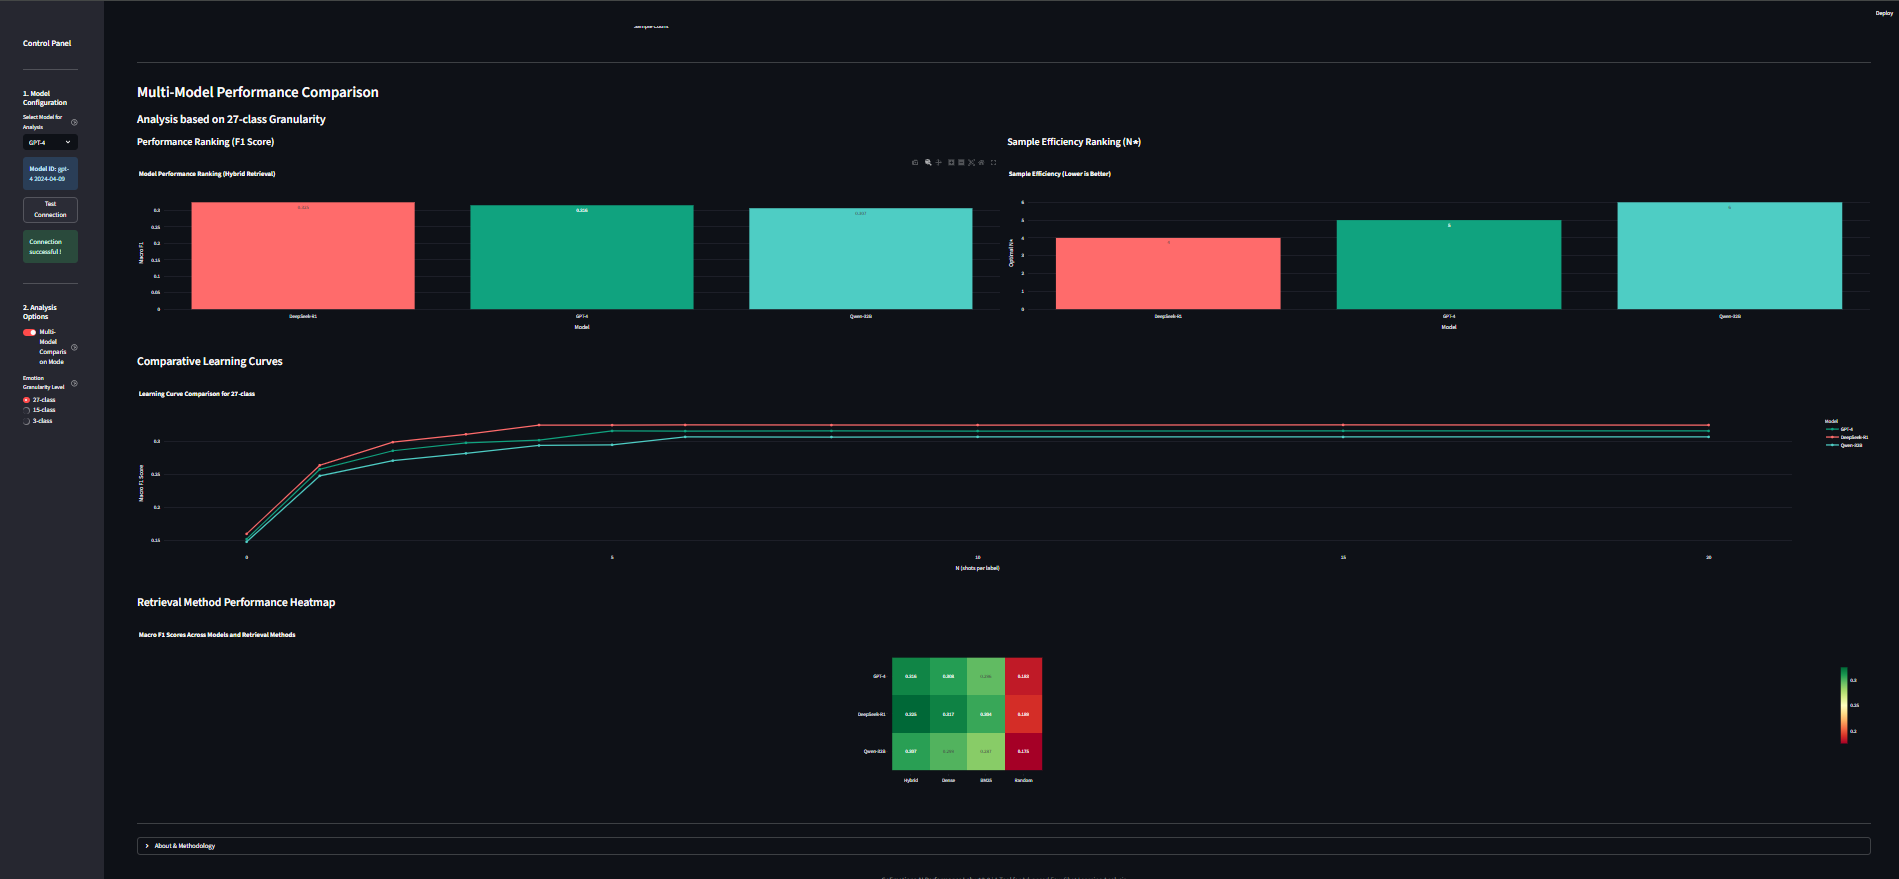
\includegraphics[width=0.9\textwidth]{Images/screenshot_multi_model.PNG}
    \caption{The Multi-Model Comparison Dashboard.}
    \label{fig:screenshot_multi}
\end{figure}

\subsubsection*{Evaluation Summary}
The implemented artifact is evaluated against the research objectives:
\begin{itemize}
    \item \textbf{Encapsulate the Full Pipeline:} The user interface successfully integrates all stages of the research into a single, cohesive application.
    \item \textbf{Facilitate Experimentation Without Code:} The GUI completely abstracts away the underlying code, allowing all experimental parameters to be controlled via interactive widgets.
    \item \textbf{Enhance Interpretability:} The system automatically generates interactive charts that make complex concepts like the performance plateau immediately apparent.
    \item \textbf{Ensure Reproducibility:} By providing a fixed set of controls, the interface ensures that any experiment is perfectly reproducible.
\end{itemize}

In conclusion, the user interface artifact is validated as a successful solution that completes the final stage of the Design Science Research cycle.